\newpage
\section{Advancing Existing FER Approaches}
\label{sec:models}

In the previous section \ref{sec:human} we concluded that a temporal dimension, and a lexical compensator might help in improving existing FER models for speaking subjects. 

We will discuss temporal compensation in section \ref{sub:temp}. A lexical compensator will have to be done with a separate model. There are different approaches to this, as we have seen in section \ref{sec:existing}. We will discuss this in section \ref{sub:lex}.

\subsection{Temporal Compensation}
\label{sub:temp}
As discussed previously, we want to keep and build on existing FER models. Given that some of our models will work on video data, we will have to temporalize our models which currently work on static images.

The straight forward approach is to take the current model, and wrap it in a temporal layer. This means that an input video with 60 frames will produce 60 output embeddings (Figure \ref{fig:temporalization}), which can then be fed into a recurrent layer like a LSTM or GRU. This produces minimal overhead, while preserving all weights from our model.

We will use this approach in all our upcoming models.

To have a comparison between frame sizes and an estimation of the importance of the temporal dimension, our models were trained on 1, 30, 60, and 90 frames.

\begin{figure}
    \centering
    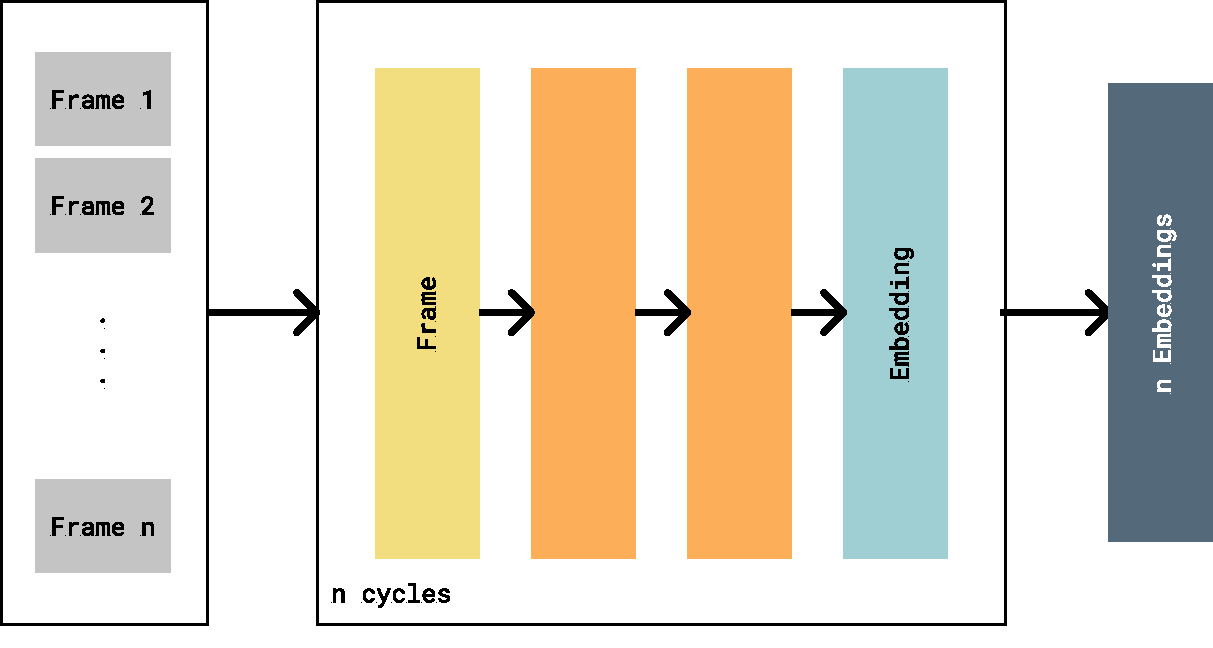
\includegraphics[width=0.8\textwidth]{res/temporalization.pdf}
    \caption{Temporalizing an FER model. The existing model gets wrapped in a TimeDimensional layer. That way the model produces $n$ embeddings for $n$ inputs.}
    \label{fig:temporalization}
\end{figure}

\subsection{Lexical Compensators}
\label{sub:lex}
We have presented two approaches to lexical compensation in sections \ref{sub:lip} and \ref{sub:style}. We will focus on those two previously mentioned approaches from Bursic \cite{bursic2020improving} and Busso \cite{salman2020style}, which attempt to extract lexical information in different ways. The goal of a lexical compensator is to extract the facial movements from speech to filter them out and extract the facial movements that are induced by the subjects emotional state.

\paragraph{LipNet} 
Bursic et al. \cite{bursic2020improving} used a LipNet embedding to detect the lexical content. We reproduced their approach to analyse the performance of the architecture, using our own MobileNet. The dataset of choice, similarly to the original model, was RAVDESS. The validation data consisted of all the recordings of actors 4 and 5.

As we have seen in section \ref{sec:lipnet_related}, LipNet requires a orofacial crop of size 100x50. A sequence of frames are passed into the network, which then gets analysed by GRU layers after a set of convolutions and poolings (Figure \ref{fig:lipnet}). We cut the network after the three layers of convolution and spatial pooling to yield an embedding for every frame. The output of the last pooling layer has a dimensionality of 96x3x6, which we passed to another MaxPooling layer of size 1x6x3 and stride 1x1x1 to create a flattended vector with 92 values and make it compatible with the concatenate step described in section \ref{sec:building}. This embedding gives us an indication of the features in the orofacial region, where the majority of lexical information in a visual feature space resides \cite{mariooryad2012factorizing}. The models then can compensate for the lexical content using this embedding.

\paragraph{Style Extractor}
The core idea of a style extractor is to separate the style (emotion) from the content (sentence/words/phonemes). Attempts at this have been published by Salman and Busso \cite{salman2020style}. This type of lexical compensator served as the inspiration for our own. We made the following changes to the architecture and preprocessing of the style extractor: we turned to FaceMesh as a facial landmark detector, yielding 468 three-dimensional coordinates, 1404 inputs in total. Additionally, we chose a smaller, non-temporal architecture network, with only one hidden layer.

We trained different models to optimize the size of the style extractor. Given that a hidden layer of 3000 neurons overtrained the model, we stepped down to 512, 256, and 128 neurons. The validation loss of the model was chosen as the deciding metric. 
All three smaller models generalized well with a very similar validation loss. We ultimately continued with the smallest model, yielding a more compact model (Figure \ref{fig:fextractor}). A style extractor with a hidden layer of size 64 was not able to match the performance of the larger models, and exceeded the validation loss of the 128-sized model of 0.1048.

Another difference to the original approach was our decision to remove the second, unused output which predicts the underlying phoneme. Test runs using a phoneme output yielded no improvement on the actual style extractor output.

The dataset used to train this model, like in the original paper, was CREMA-D.

\begin{figure}
    \centering
    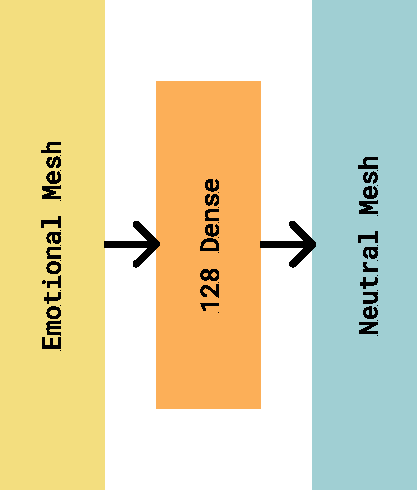
\includegraphics[width=0.5\textwidth]{res/FExtractor.pdf}
    \caption{The architecture of our final feature extractor. The emotional input mesh of a subject speaking a given phoneme $p$ gets passed to a densely connected hidden layer with 128 neurons. The output of the network is a prediction of a neutral mesh of the actor pronouncing the same phoneme $p$.}
    \label{fig:fextractor}
\end{figure}

\subsection{Building the Models}
\label{sec:building}

To complete the architecture, we will briefly talk about the fusion layers. In instances where two model inputs come together (e.g. the lexical compensators) we need a network that combines both inputs. We want this fusion network to be consistent across all our models to make sure that differences in results are not due to differing architectures.

We turned to the fusion layer by Bursic et al. \cite{bursic2020improving}. We tried to replicate their approach with the lexical compensation from LipNet, and our FER model had a similar embedding with 512 neurons to their VGG19 model. This lets us better compare our results to theirs. In comparison to the model from Salman and Busso \cite{salman2020style}, this fusion network covers all seven core emotions.

To judge the impact of the lexical compensators we also trained a model that only uses the temporalized embedding of our FER model. We use the same fusion network, this time in a transfer learning approach. The FER embedding of 512 neurons gets passed to the same fusion network, foregoing the \texttt{concatenate} step. This aides in comparing the impact of the lexical compensators without having any noise from a differing transfer network.

The input from the previous model(s) are fed into a bidirectional GRU layer of size 256. A dense layer of size 16 follows. The final output layer is a densely connected layer of size 7, corresponding to the core emotions. The activation function of the hidden layers are ReLU, while the output layer has a softmax activation function. A dropout layer of 0.5 is placed between the GRU and the following dense layer (see Figure \ref{fig:fusionlayers}).

We end up with three main architectures, which we will train, validate, and compare:

\begin{enumerate}
    \item \textbf{Temporal FER model: FER-TC} The temporalized FER model without a lexical compensator, with 512 inputs.
    \item \textbf{Lexical compensation with LipNet: FER-LN} The temporalized FER model with LipNet as the lexical compensator, with 512 (FER) + 96 (LipNet) inputs.
    \item \textbf{Lexical compensation with our Style Extractor: FER-SE} The temporalized FER model with a self trained style extractor as the lexical compensator, with 512 (FER) + 1404 (Style Extractor) inputs.
\end{enumerate}

\begin{figure}
    \centering
    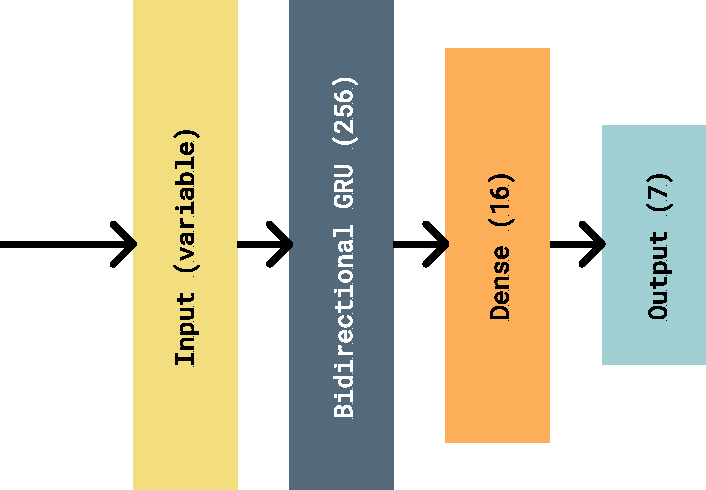
\includegraphics[width=0.7\textwidth]{res/FusionLayers.pdf}
    \caption{The architecture of the fusion/transfer network. It is kept simple to accommodate the smaller datasets we use and follows the architecture from Bursic et al. \cite{bursic2020improving}.}
    \label{fig:fusionlayers}
\end{figure}
\subsection{Data and Preprocessing}
\paragraph{Data for FER Models}
We mainly use two datasets in our work, RAVDESS and CREMA-D. Since the actual usage of the data is dependent on some common preprocessing steps like face-/mouth-cropping and landmark extraction, we transformed the datasets before starting training.

The FER-model takes a facial crop of the frame, with 224x224x3 dimensions (width, height, colour channels). The facial crop had to be proportional to the original image, so it was important not to stretch or morph the cropped frame (Figure \ref{fig:crop}). In preprocessing, we saved a crop of every frame for all videos. 
The LipNet model required a 100x50x3 dimensional input of the orofacial area. This crop was saved alongside the facial crop for each frame. Both the facial and orofacial crops were done with the frontal face detector of dlib \cite{dlib09}. Finally, our style extractor was be trained on facial landmarks extracted from FaceMesh. Those were also stored with the facial and orofacial crops.

Each videos data is saved as an array in a \texttt{pickle} file. The structure of the file can be seen in figure \ref{fig:pickle}.
\begin{figure}
    \centering
    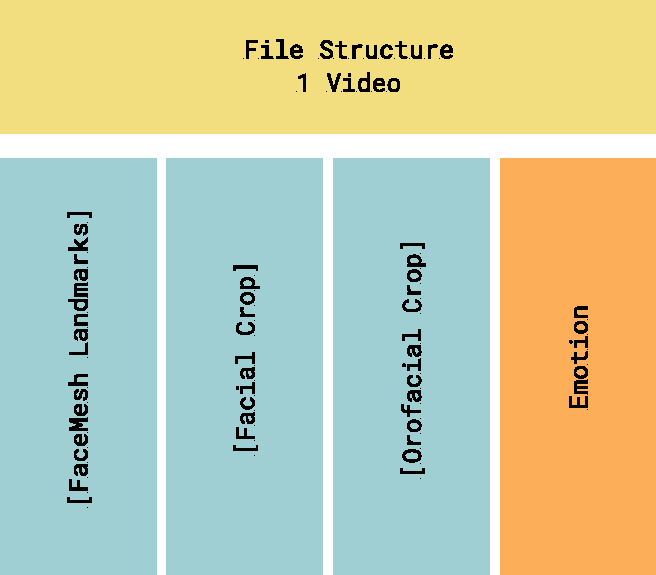
\includegraphics[width=0.5\textwidth]{res/Pickle.pdf}
    \caption{The data structure of our preprocessed files. Each file corresponds to one video. Its facial and orofacial crops, alongside with its facial landmarks are stored in arrays. The array lengths correspond to the amount of frames in each video. The underlying emotion is saved as well.}
    \label{fig:pickle}
\end{figure}

\begin{figure}
    \centering
    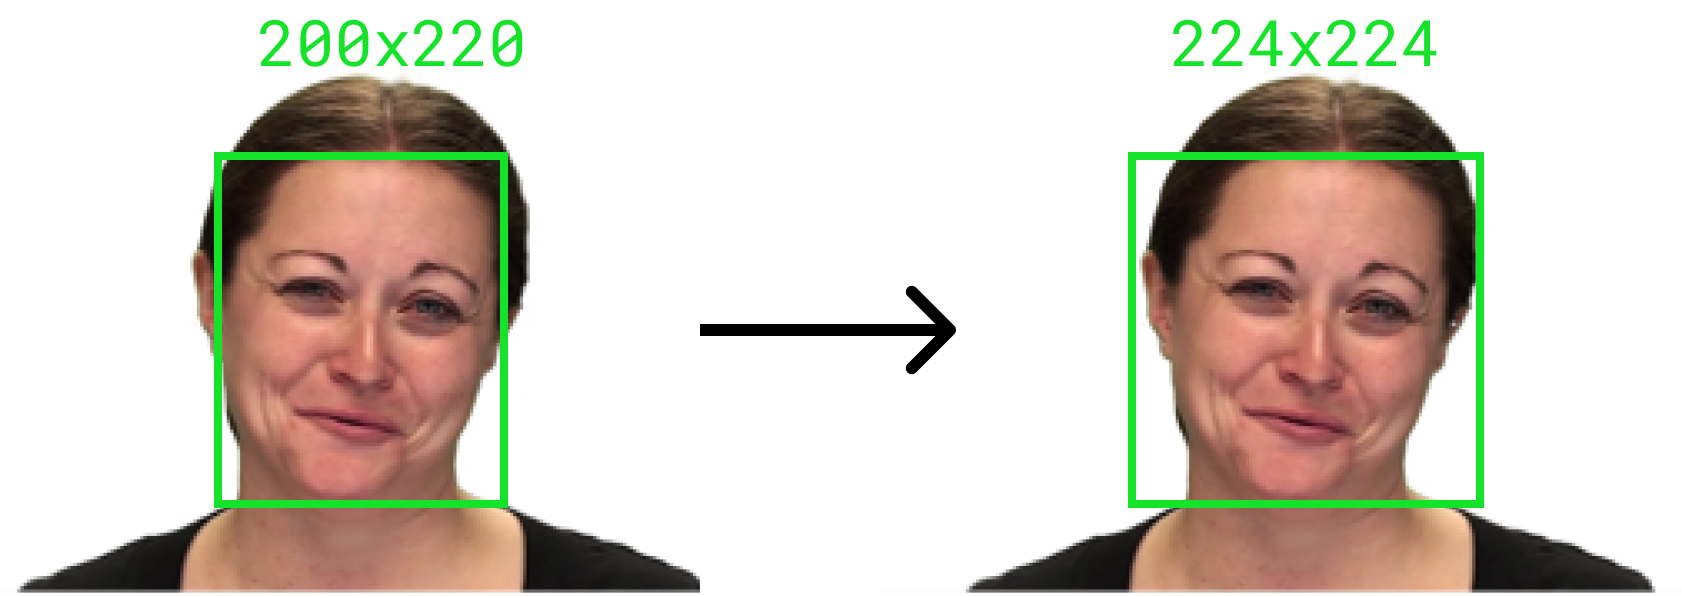
\includegraphics[width=0.8\textwidth]{res/croppng.png}
    \caption{The input for the FER model had to be a crop of the subjects face, with a dimension of 244x244 pixels. It was important not to stretch the original crop and keep the proportions. We extended the facial bounding box to fit it to the required dimensions.}
    \label{fig:crop}
\end{figure}


\paragraph{Data for the Style Extractor}
To be able to train the style extractor we need pairs of meshes for every phoneme, where one mesh is emotional (not neutral) and one neutral. To have a more fine-grained model, we also made sure that all mesh pairs are from the same occurrence. As an example, the sentence "It's eleven \textbf{o}'cl\textbf{o}ck" has two occurrences of the phoneme \texttt{O} (marked). When training the style extractor, all mesh pairs came from the same actor in the same sentence from the same occurrence. We achieved this by using the MFA (see section \ref{sub:mfa}) to align the video files. Phonetic transcripts that do not have neutral counterparts were ignored. This left us with around 140.000 phoneme pairings to train the style extractor with. 


\subsection{Training}
Here we present more detailed information for the training process of our models, and discuss results from model validation.
\paragraph{General Information}
To keep the models comparable on the temporal dimension, we trained each model on 1, 30, 60, and 90 frames. The FER and LipNet model were pre-trained and frozen. We wanted to cover the core emotions that were defined by Ekman, and thus ignored the \texttt{calm} emotion that was provided by the RAVDESS dataset. Those files did not appear during training or validation and were discarded.

We used a sliding window approach on the frame arrays. Given a model with a frame size of 60 and a video with 100 frames, we now have the opportunity to extract multiple data point from the video. We used a window stride of 5. This means that the first data point ranges from frame 0 to 59, the second from 5 to 64 and so on. This helped to somewhat ease the problem of the RAVDESS dataset being too small for proper DNN training. 

Our specific style extractor was trained separately. It was trained on CREMA-D, with actors 1 to 11 being used for validation.

The fusion networks for all models was trained on RAVDESS. Actors 4 and 5 were used for the validation set, the files from the other 22 actors were used for training.

We used an early stopping and snapshot callback during training. If the validation loss dropped on three consecutive epochs, training was finished. The most accurate model on the validation set was saved and later used for further analysis in section \ref{sec:model_results}.

\paragraph{Technical Details}
We used the \texttt{keras} environment using a \texttt{tensorflow} backend (version 2.4.1) to train our models on a HPC using an Nvidia Titan X GPU with the Pascal architecture. The scripts were deployed in Docker containers, on a server running Ubuntu 18.04 LTS.

The preprocessed datasets were stored separately on the HPC and were injected into the docker container through virtual links. The \texttt{Dockerfile} was based on the \texttt{nvidia/cuda:11.0-runtime-ubuntu16.04} runtime, using version 3.6.8 of Python.

The \texttt{SlidingWindowGenerator} for training and validation data was implemented as an extension of the \texttt{Sequence} class from \texttt{keras}. It allows the \texttt{model.fit()} function to iteratively fetch batches of data using the implementation of the \texttt{\textunderscore\textunderscore getitem\textunderscore\textunderscore()} function. Window stride, window size, and batch size were dynamically adjustable. We implemented Sliding Window Generators for each trained model.

\subsection{Discussion}
In this section we present the results of training and validating our models. We will first discuss the results from the validation set of the training dataset RAVDESS, and then explore the performance of the models on other datasets.
\subsubsection{Validation Results}
\label{sec:model_results}
In this section we will present the results of our training. We saved all \texttt{history} objects from training, alongside the model with the highest validation accuracy. For more detailed analysis for confusion matrices we manually ran predictions on the validation part of the dataset. 

The results in figure \ref{fig:max_acc} show the accuracies of the validation data for each model on the respective frame window size. 
% \begin{table}[h!]
%     \centering
%     \begin{tabular}{cccc}
%     \hline
%   \textbf{\# Frames}  & \textbf{LipNet}  & \textbf{Style Extractor}  & \textbf{No Compensator}  \\ \hline
%     1 & 0.66 & \textbf{0.67}  & 0.66 \\ 
%     30 & 0.67 & \textbf{0.71} & 0.70 \\ 
%     60 & 0.76 & 0.74 & \textbf{0.77} \\ 
%     90 & \textbf{0.84} & \textbf{0.84} & 0.83 \\ 
% \end{tabular}
%     \caption{Test data accuracy of the three different models trained on RAVDESS. The models with the highest accuracy in the frame group are indicated in bold.}
%     \label{tab:restab}
% \end{table}

A general trend becomes obvious: the temporal dimension, and an increase in frame-window size is improving model performance. This increase is at around five to six percentage points per 30 frames. Judging by the pure accuracy results, both lexical compensators provide little to no improvement in model performance, no matter the amount of frames. A potential reason for this trend might be that the lexical content already gets compensated through the temporal dimension, evening out the noise it creates. We will discuss the effect of the lexical compensators in further experiments and analysis in section \ref{sec:cross_dataset} when we analyse cross dataset performance.

\begin{figure}
    \centering
    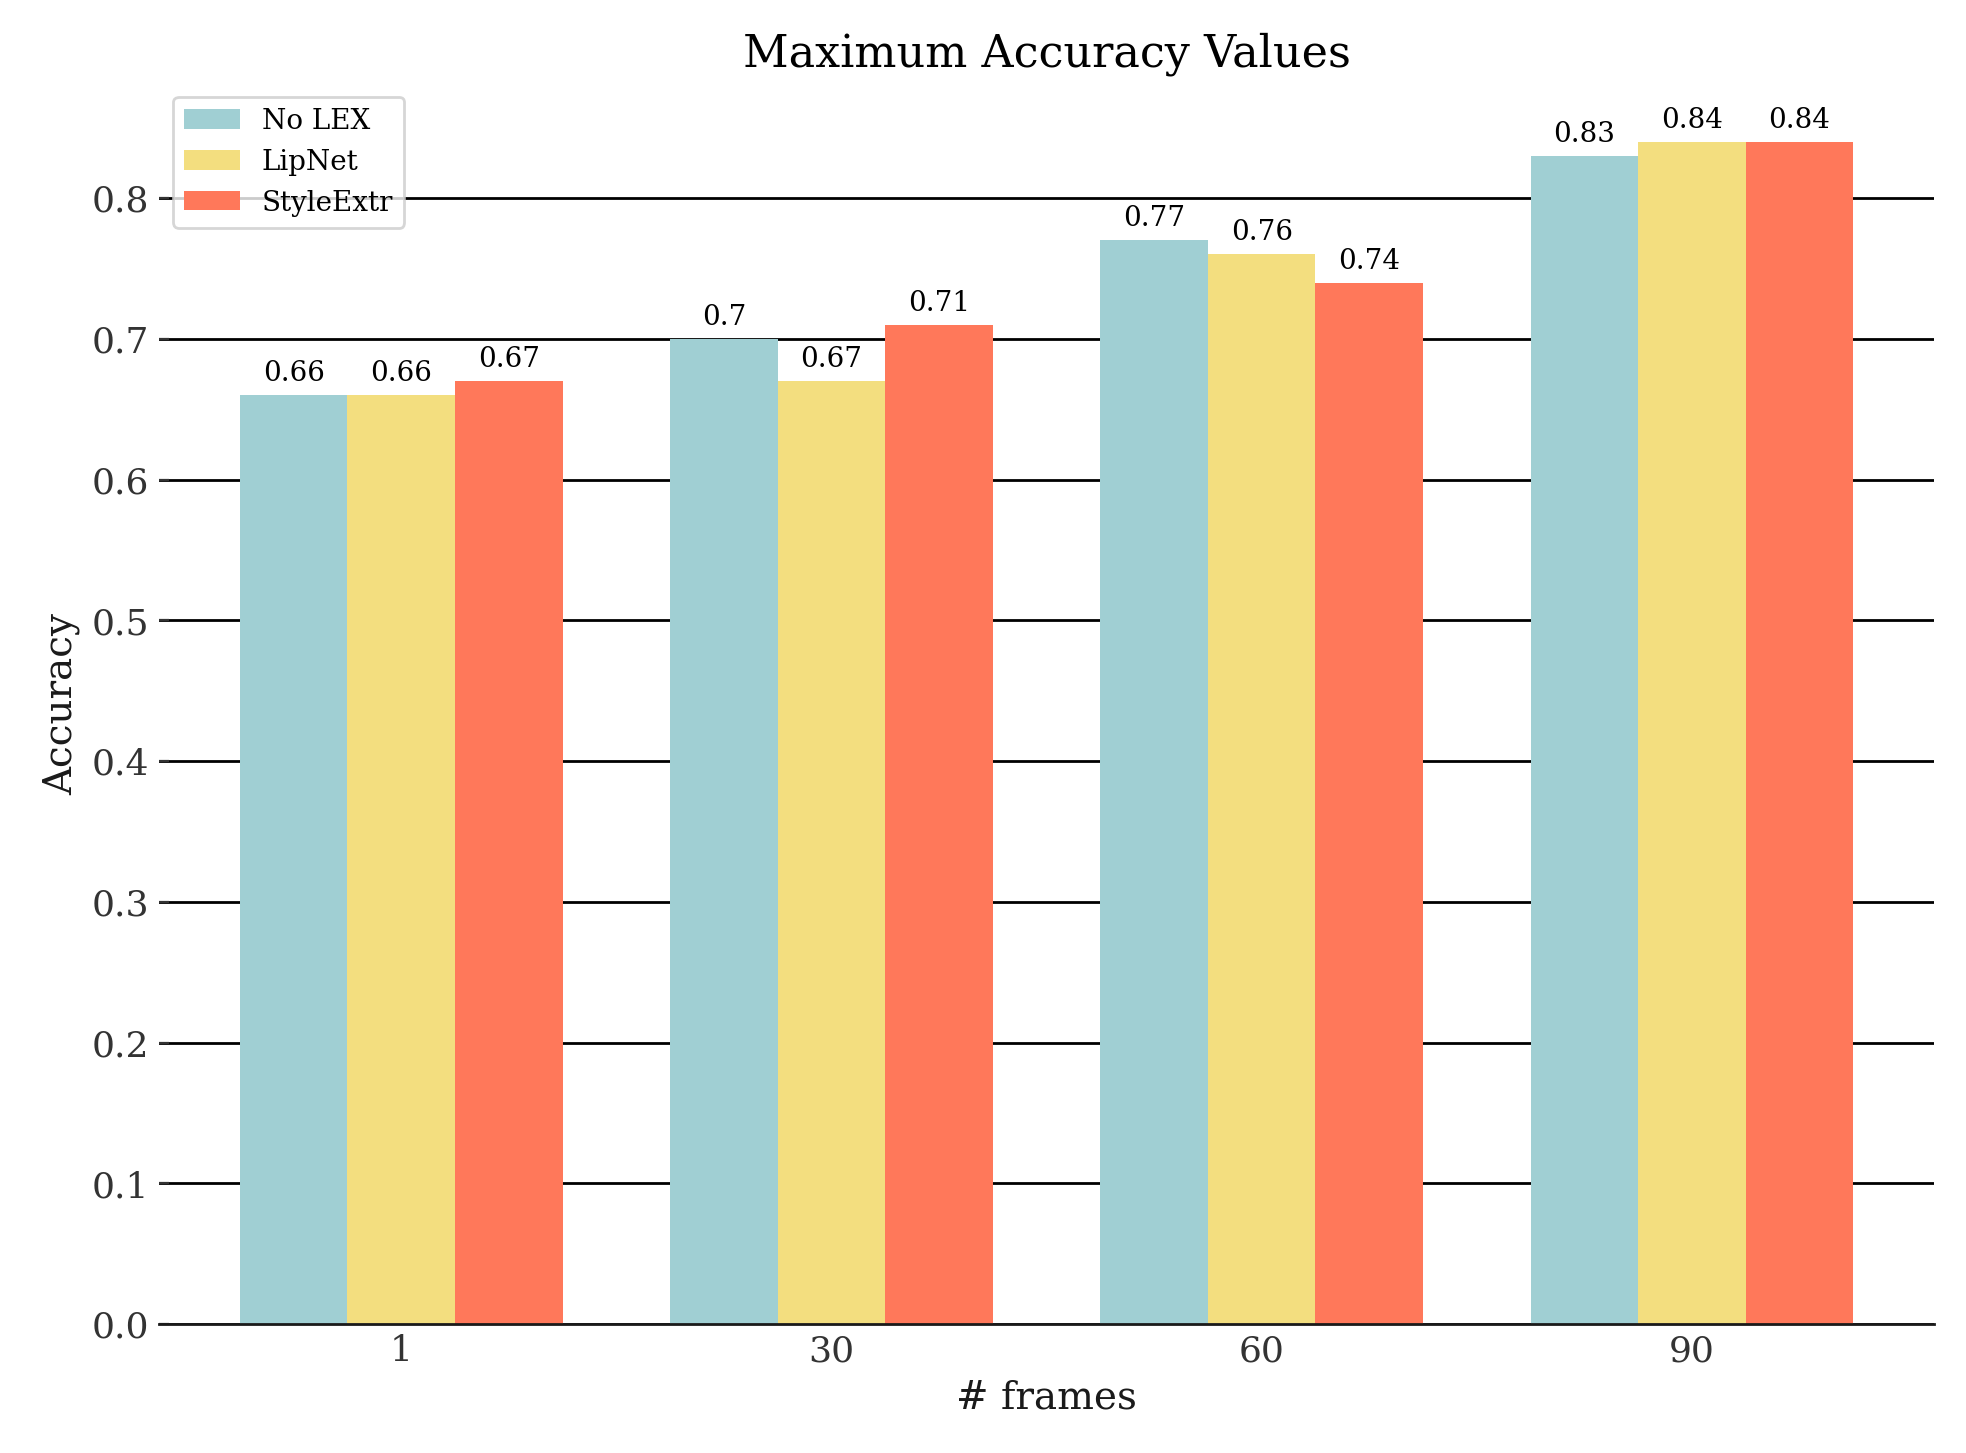
\includegraphics[width=0.8\textwidth]{res/maxaccvalues.png}
    \caption{The maximum validation accuracies during training for our three models. The temporal dimension improves the accuracy, whereas neither lexical compensator shows significant improvements in performance.}
    \label{fig:max_acc}
\end{figure}

\begin{figure}
    \centering
    \begin{subfigure}[b]{0.45\textwidth}
      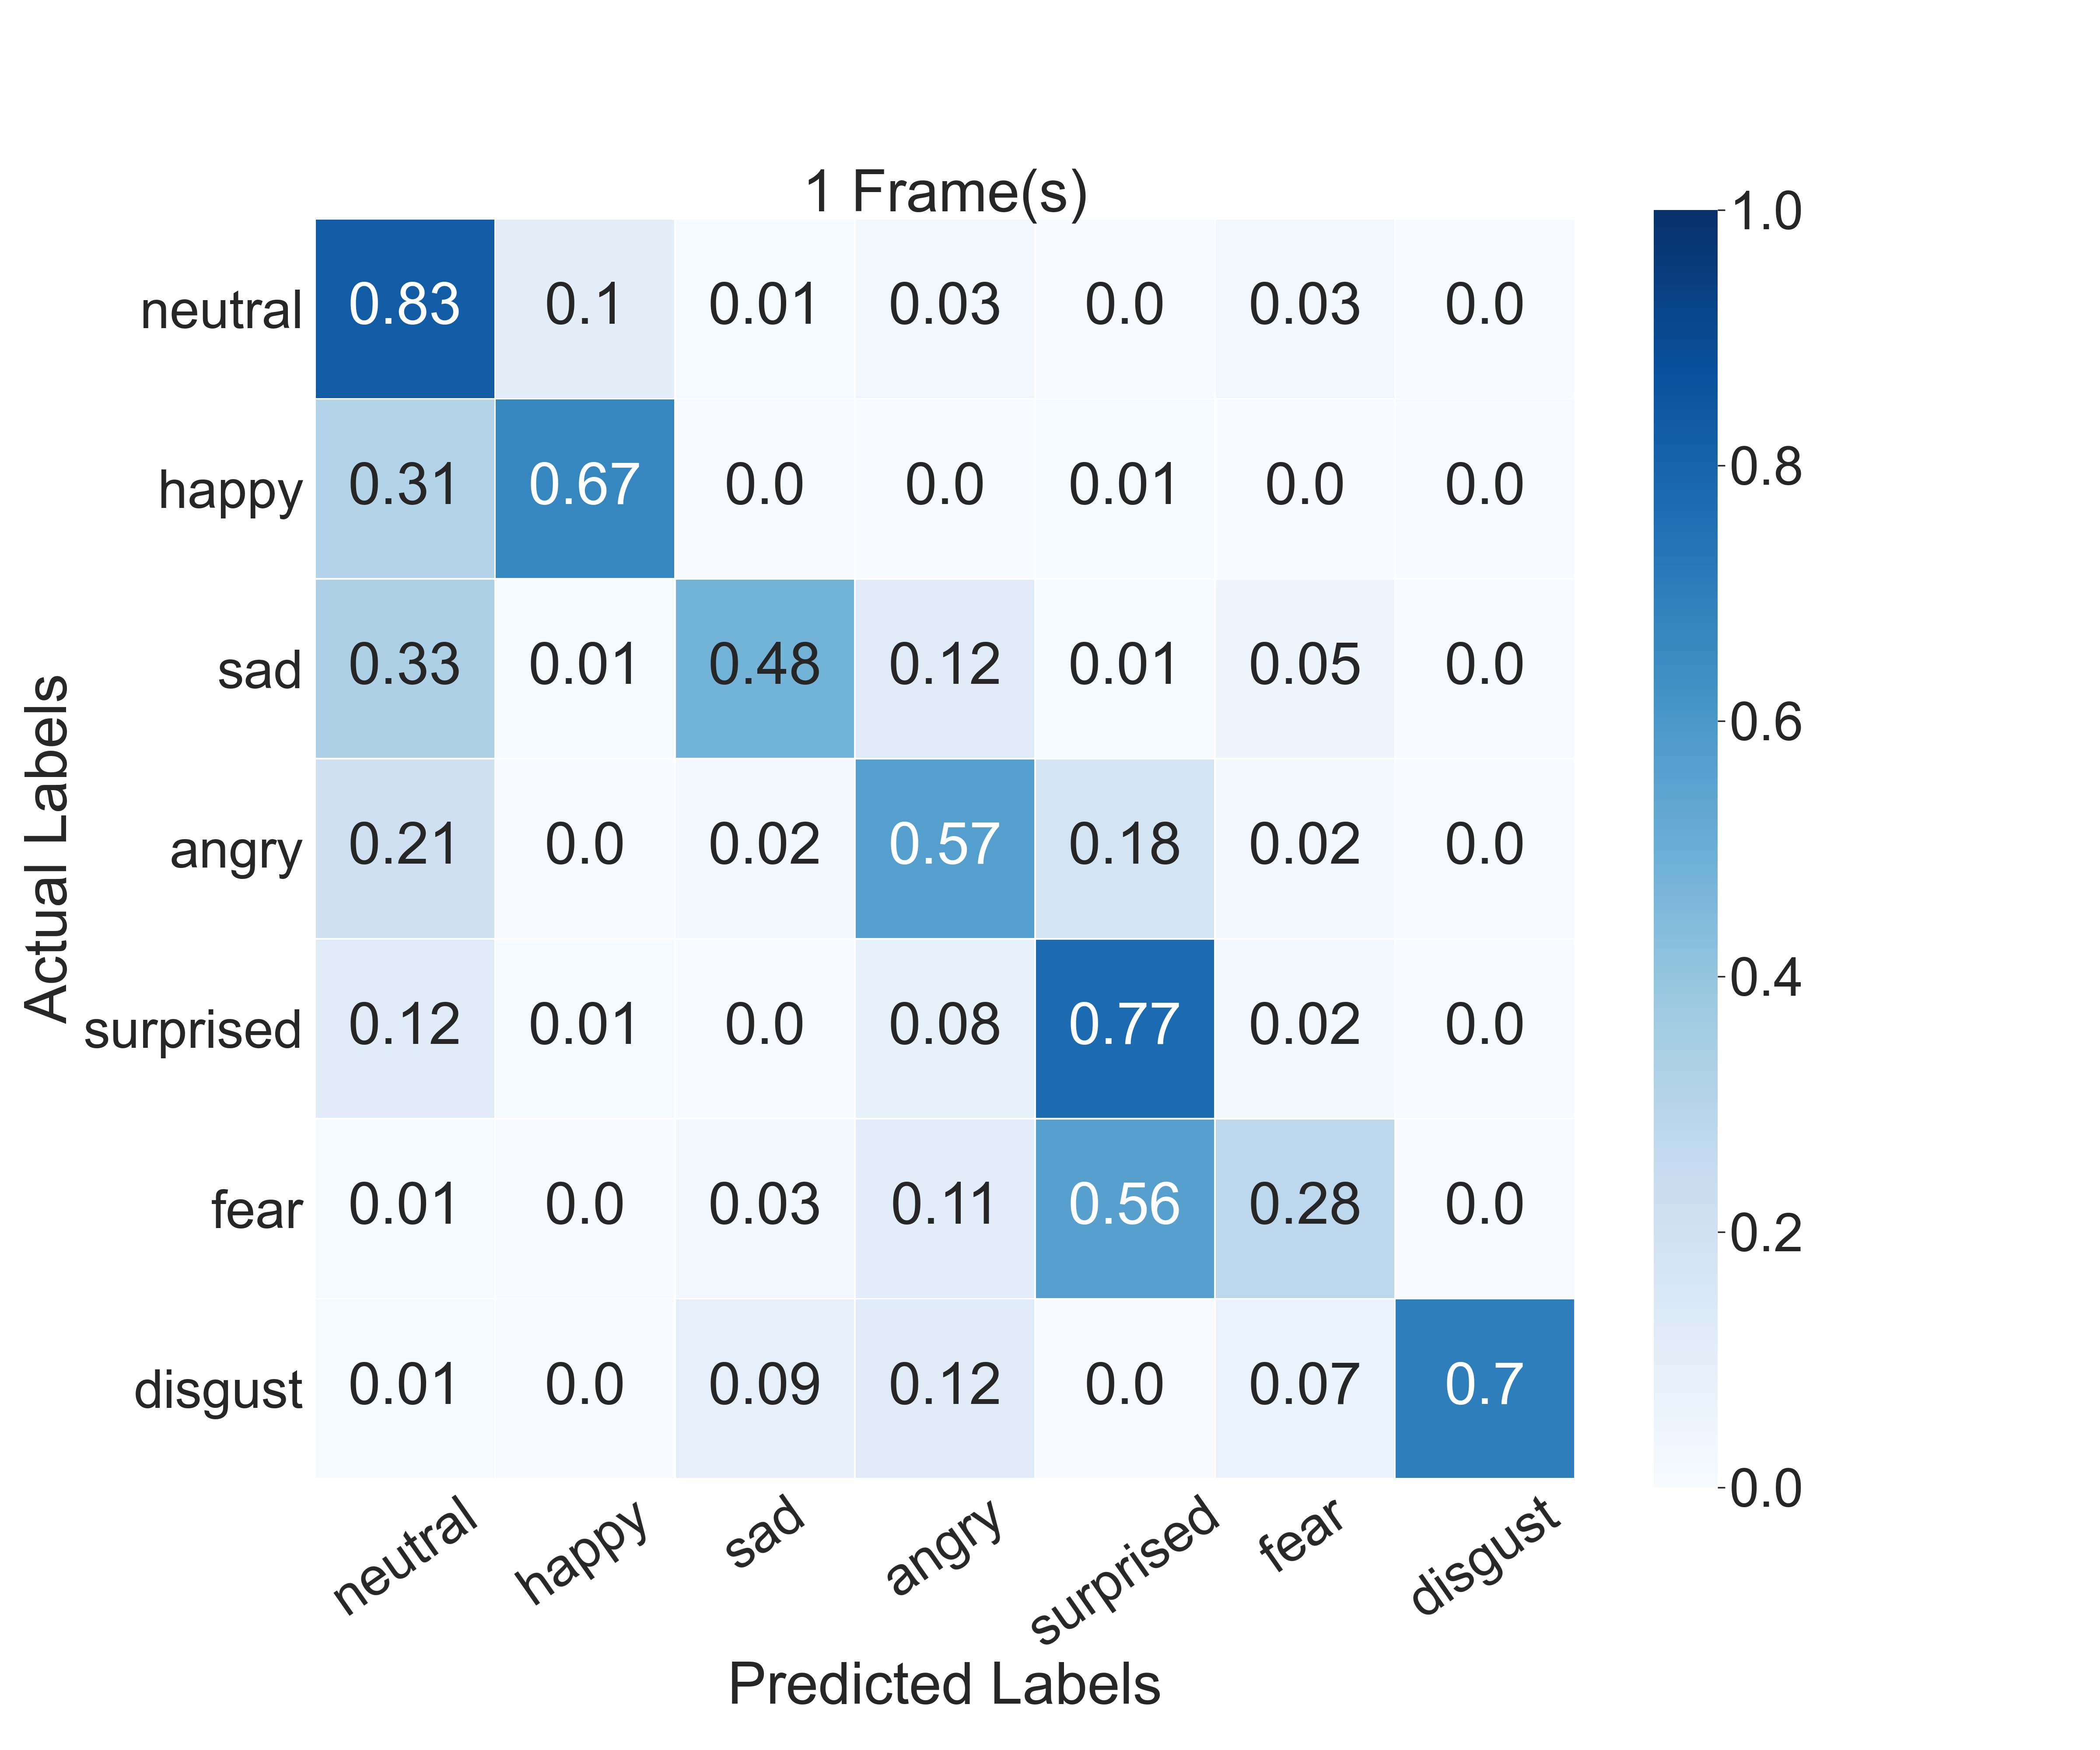
\includegraphics[width=\textwidth]{res/conf_fer_1.png}
    \end{subfigure}
    \begin{subfigure}[b]{0.45\textwidth}
      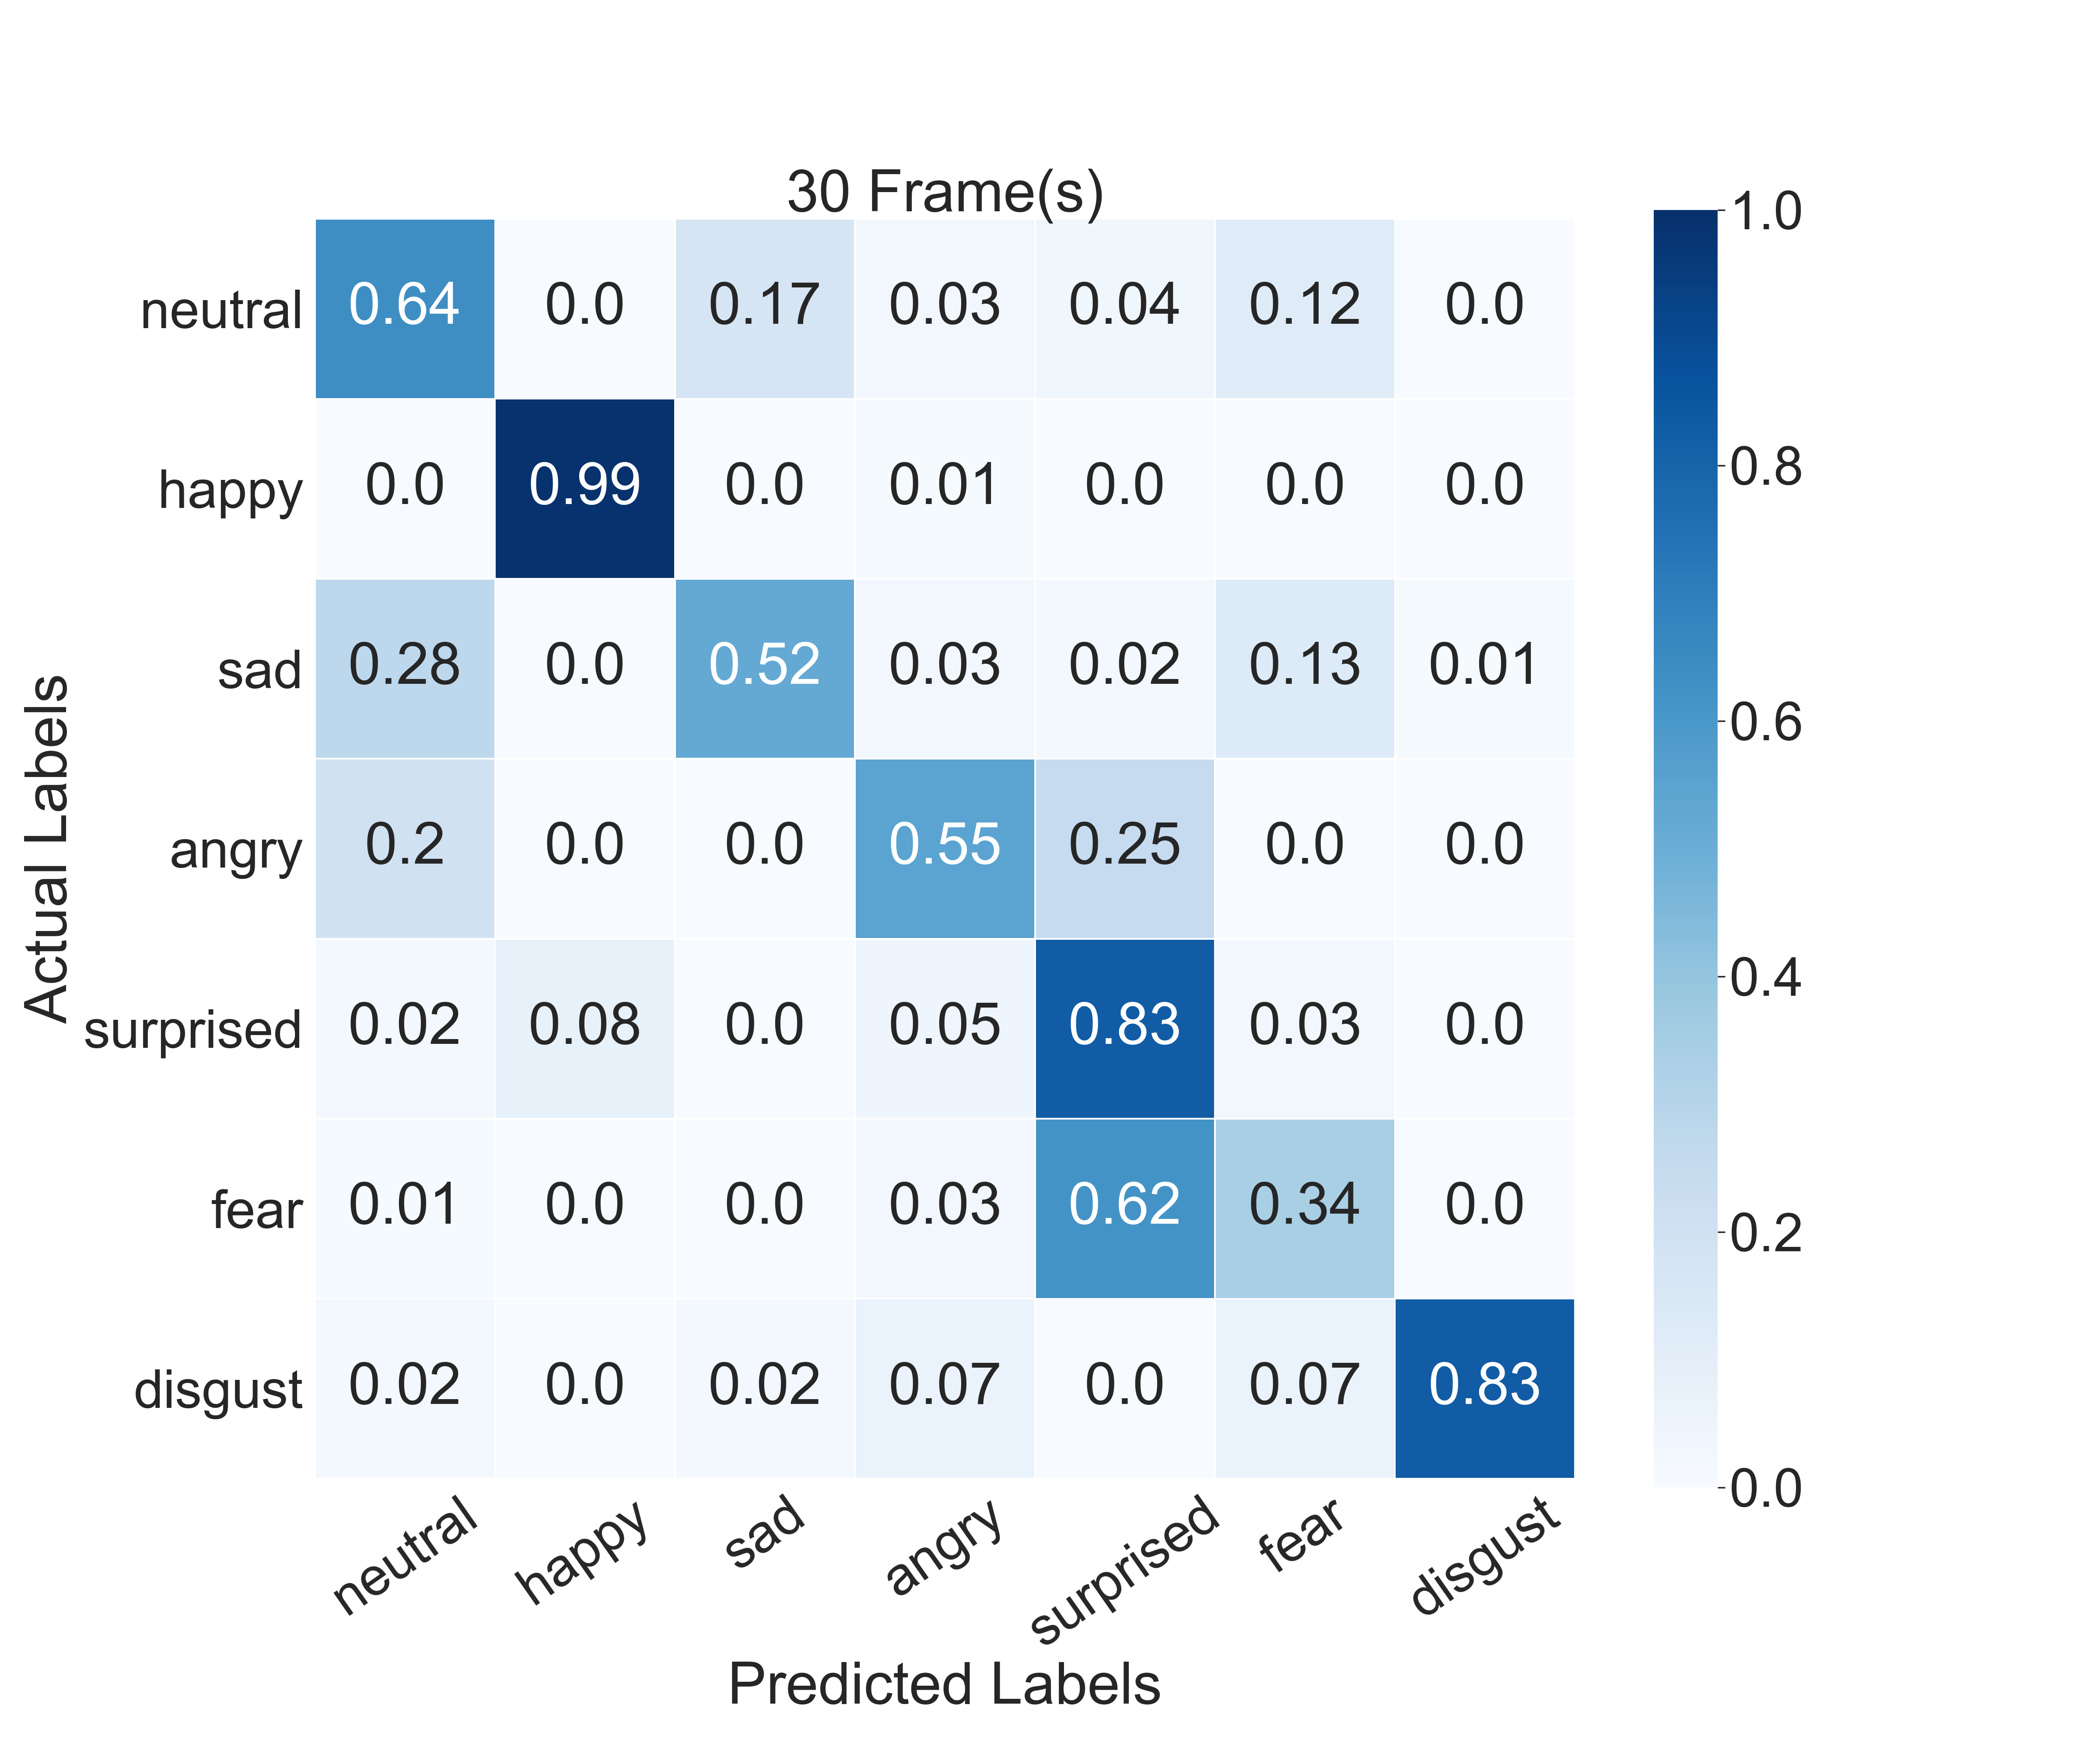
\includegraphics[width=\textwidth]{res/conf_fer_30.png}
    \end{subfigure}
    \begin{subfigure}[b]{0.45\textwidth}
      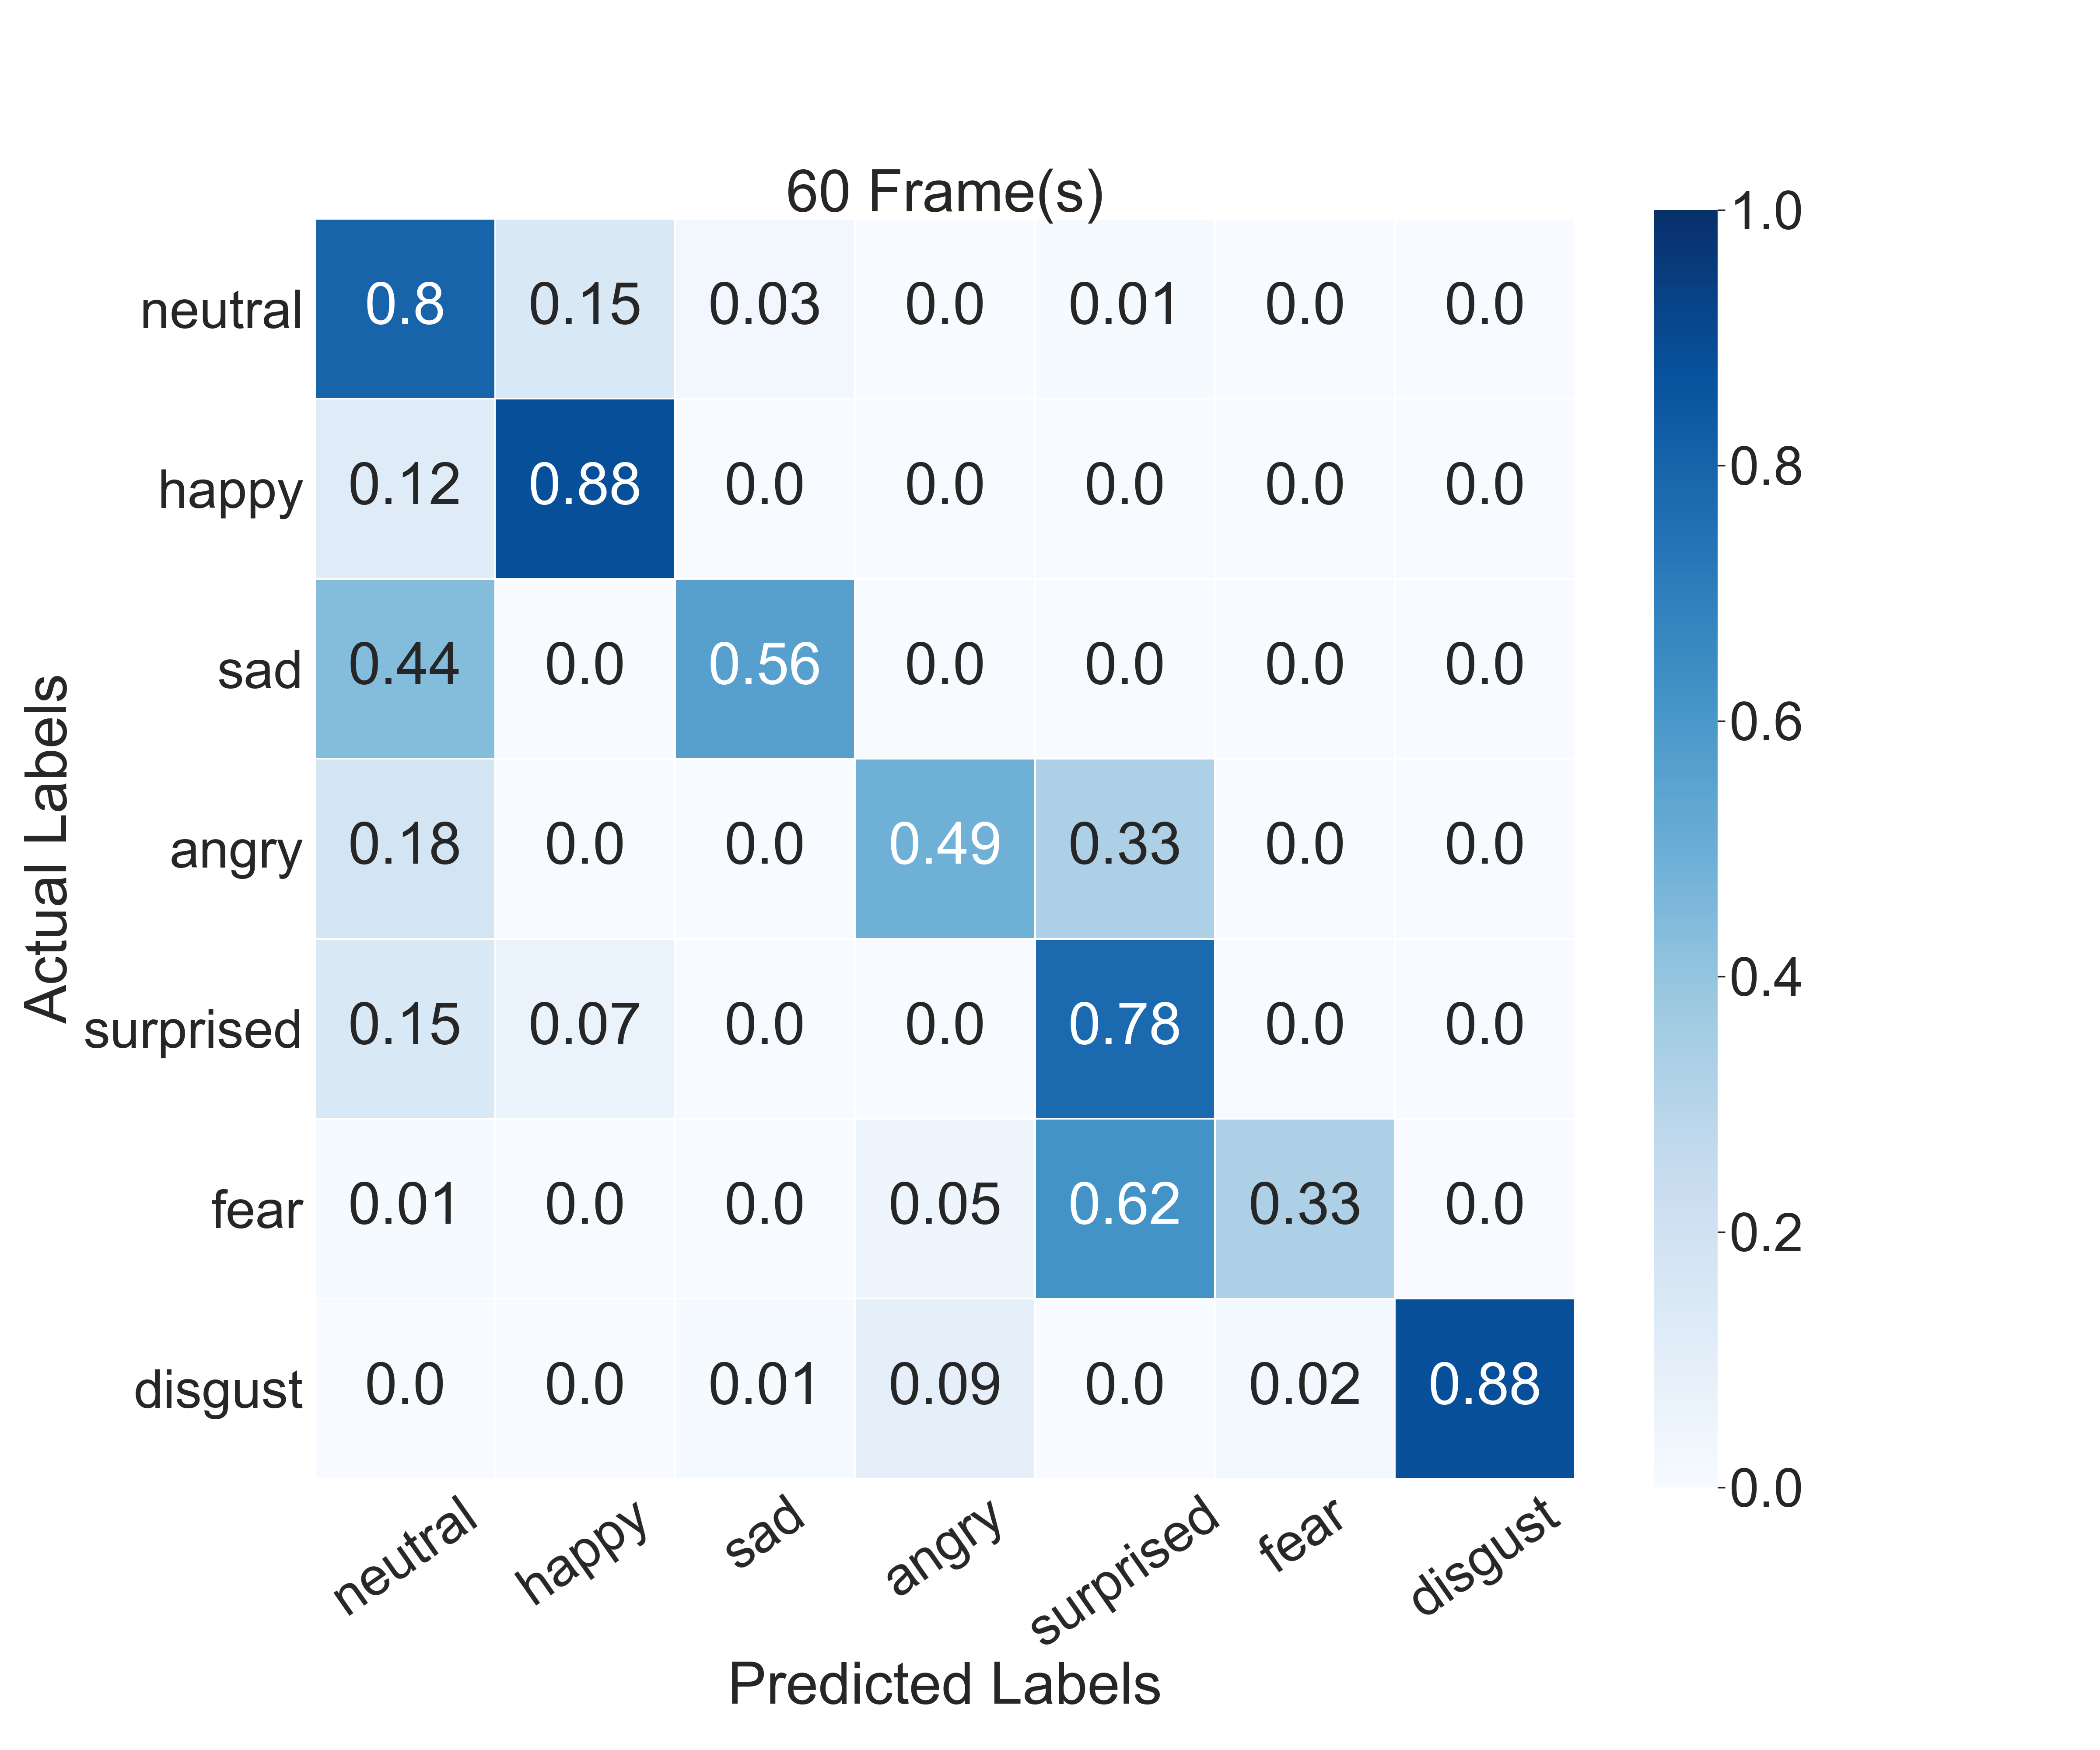
\includegraphics[width=\textwidth]{res/conf_fer_60.png}
    \end{subfigure}
    \begin{subfigure}[b]{0.45\textwidth}
      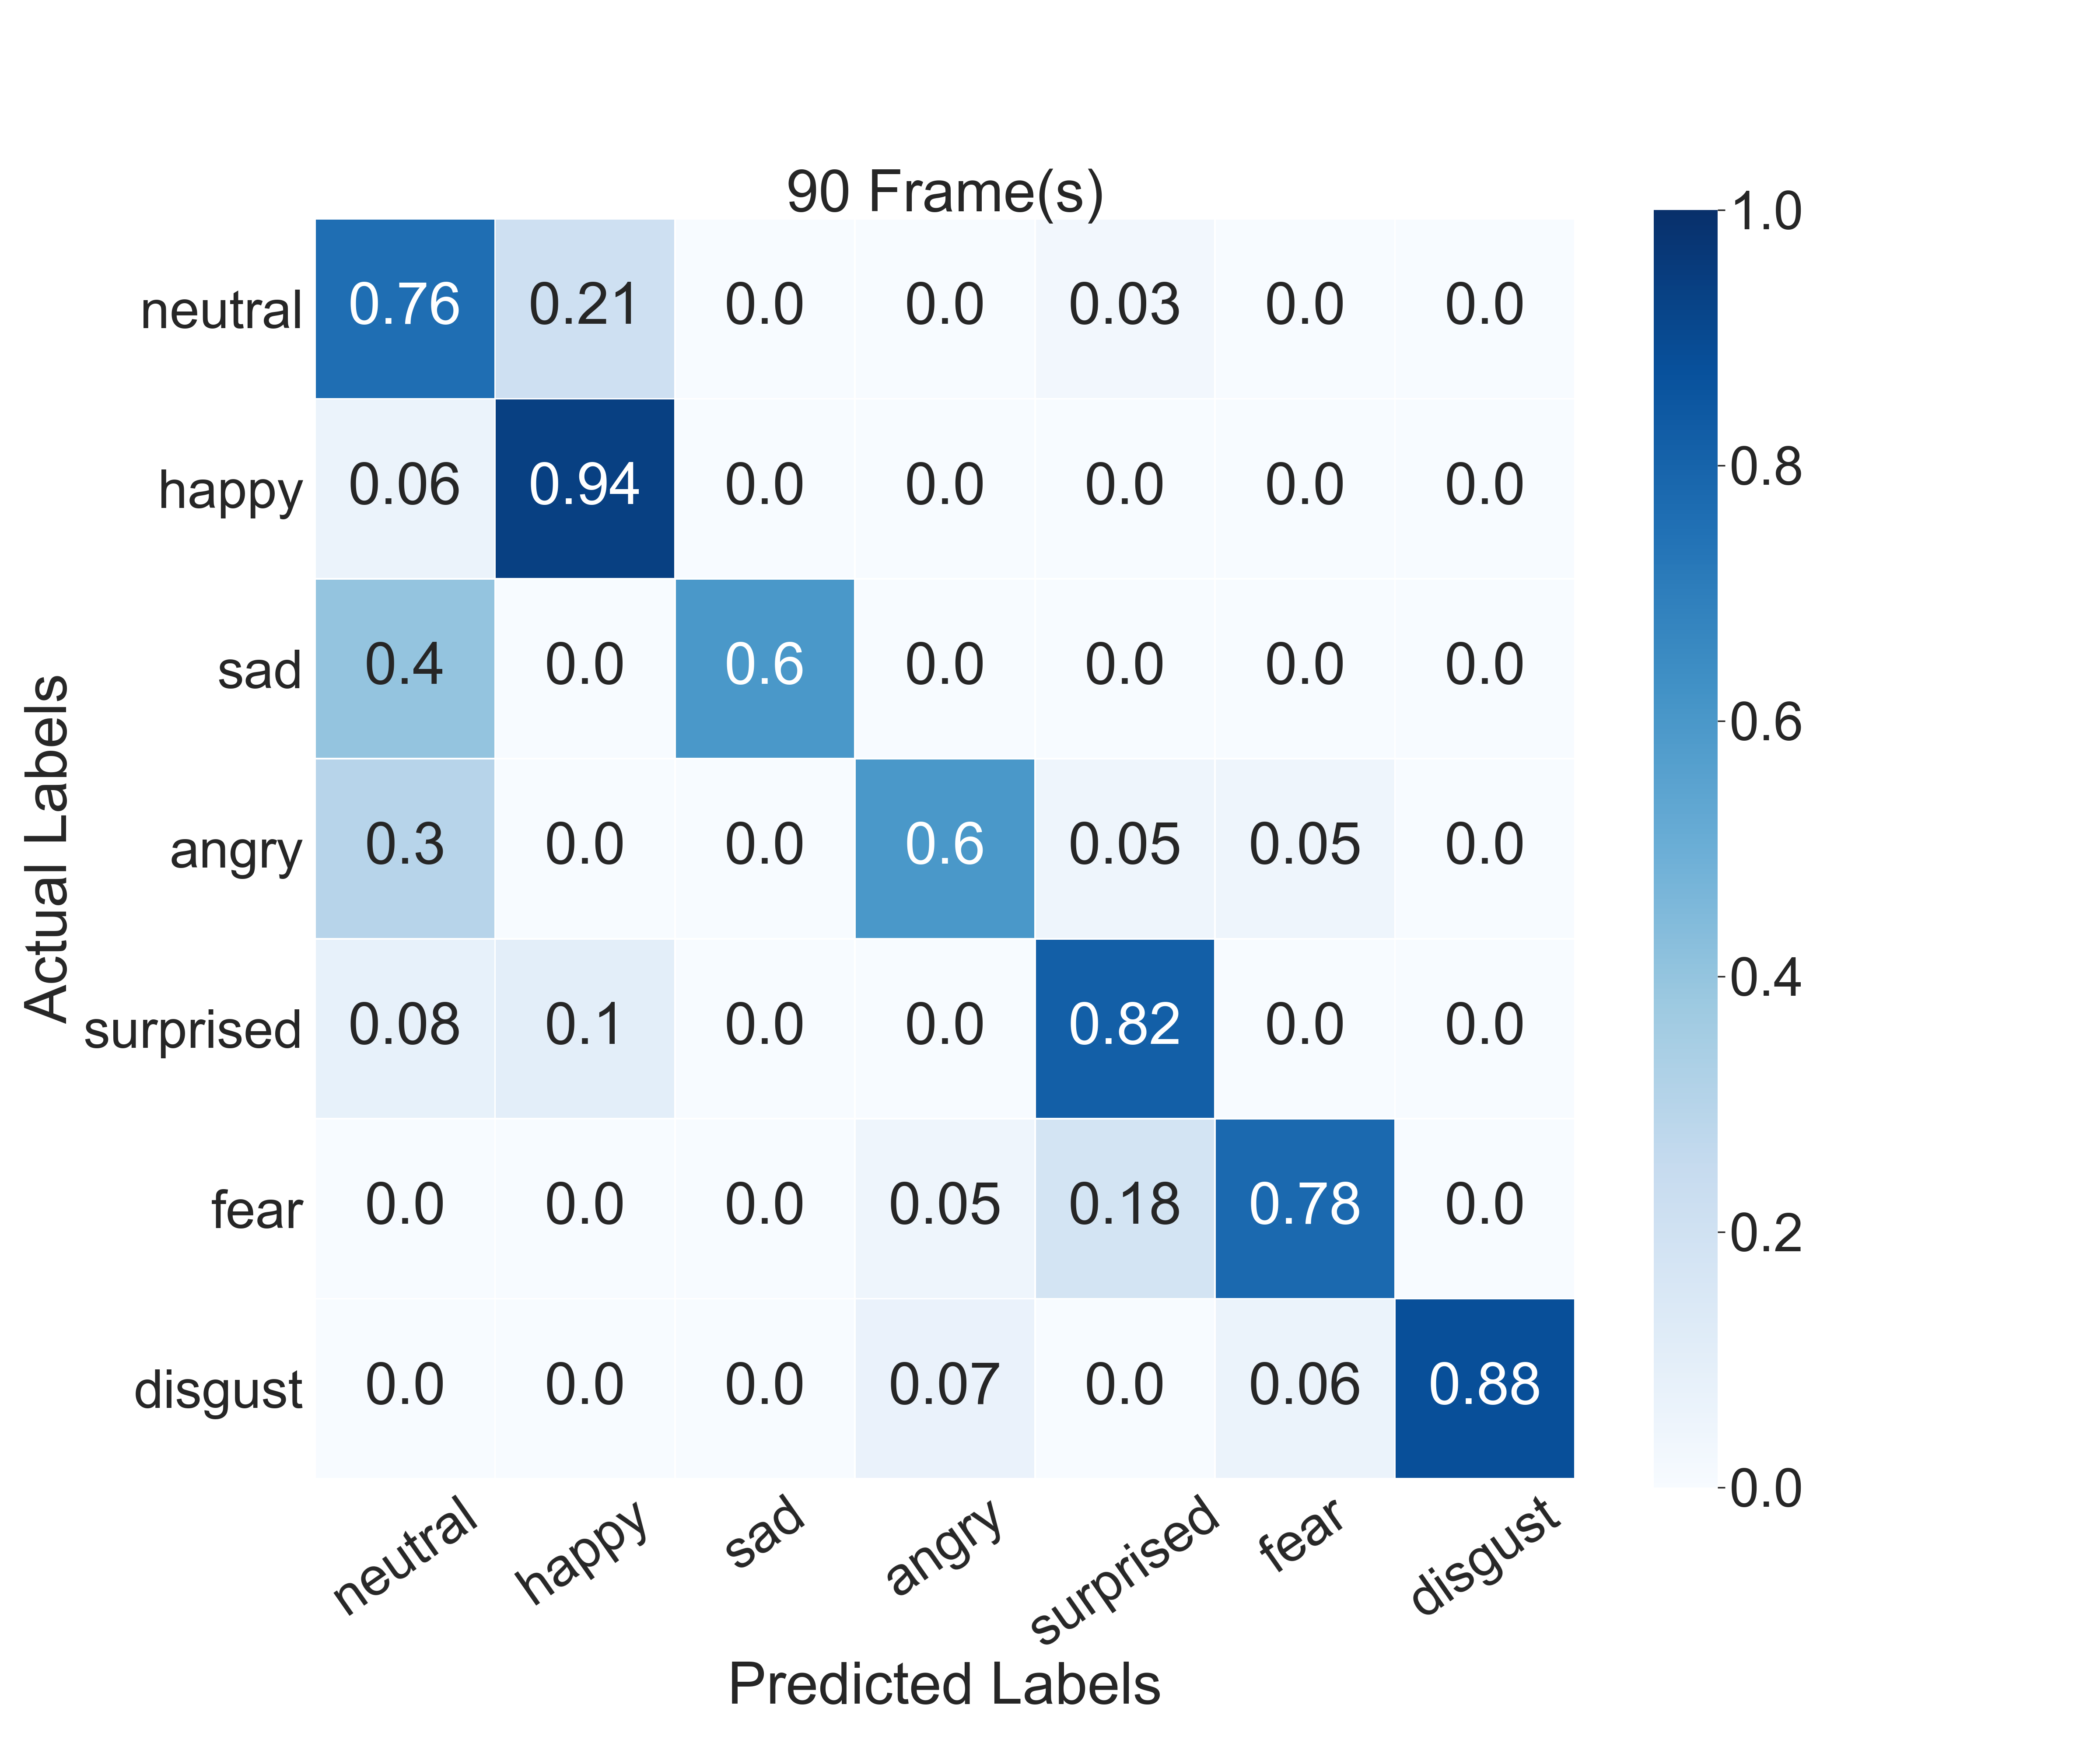
\includegraphics[width=\textwidth]{res/conf_fer_90.png}
    \end{subfigure}
    \caption{Confusion matrices of the validation data for the FER model without a lexical compensator (FER-TC).}
    \label{fig:fer_conf}
\end{figure}

\begin{figure}
    \centering
    \begin{subfigure}[b]{0.45\textwidth}
      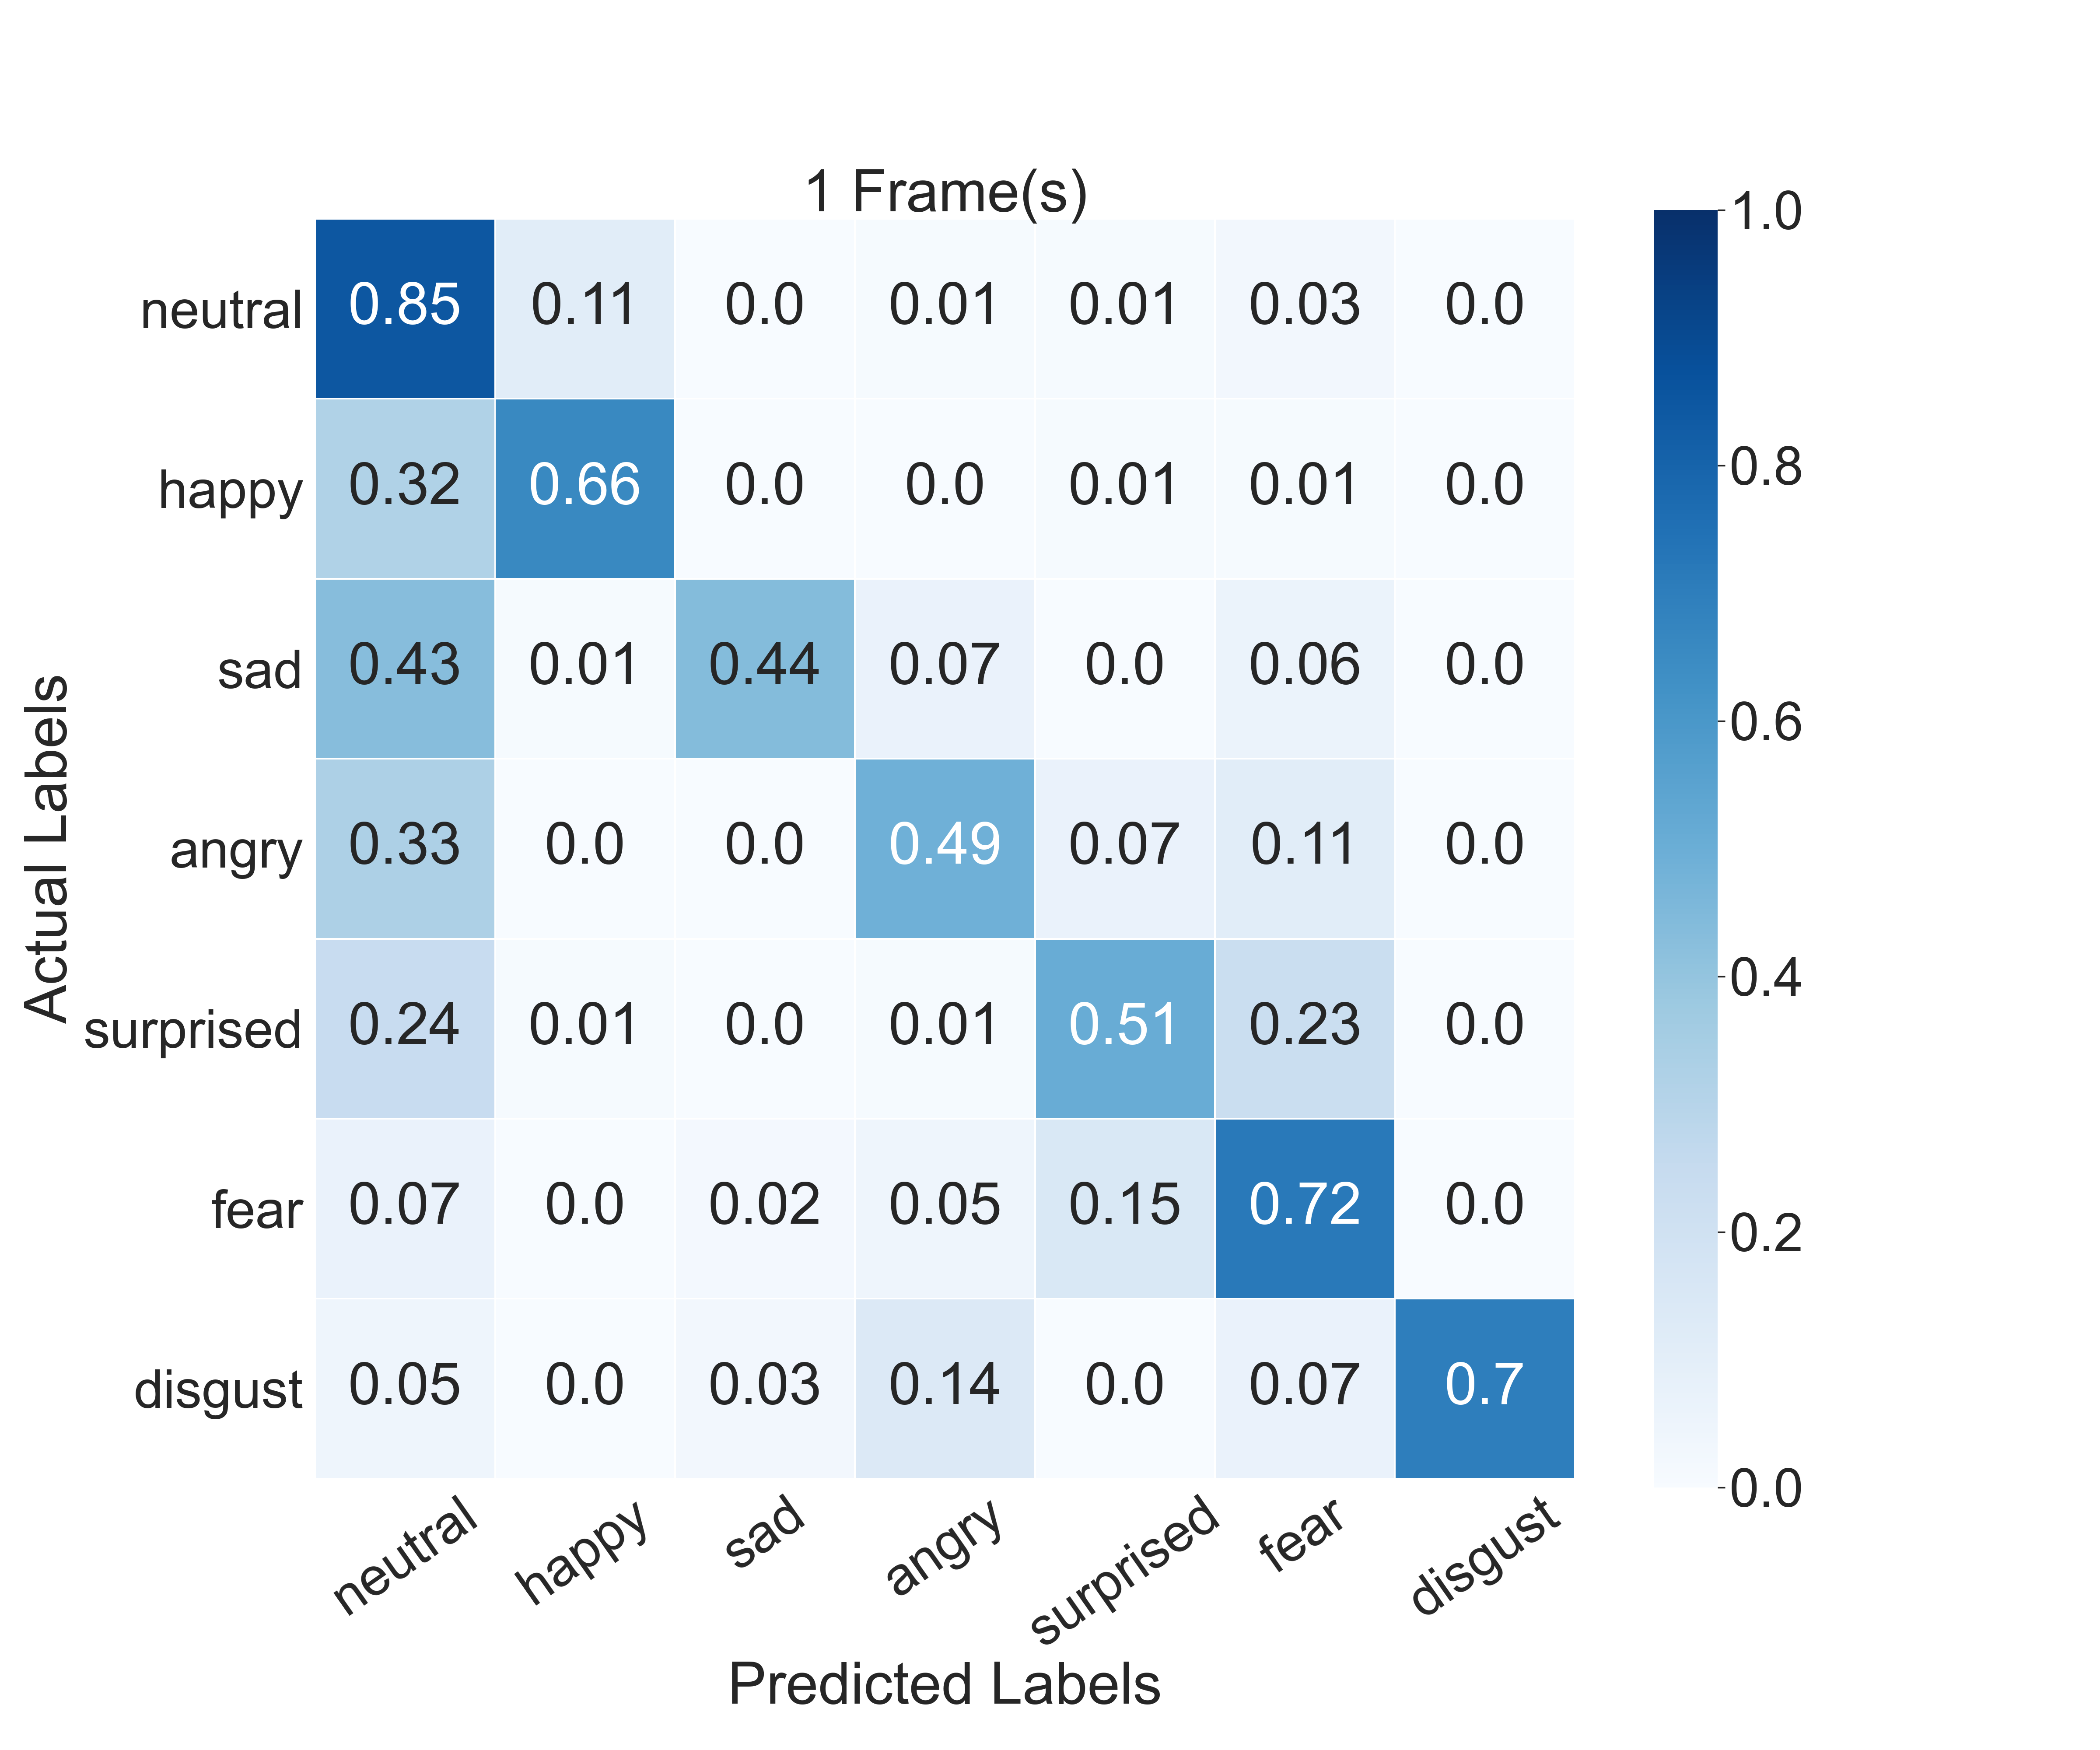
\includegraphics[width=\textwidth]{res/conf_fusion_1.png}
    \end{subfigure}
    \begin{subfigure}[b]{0.45\textwidth}
      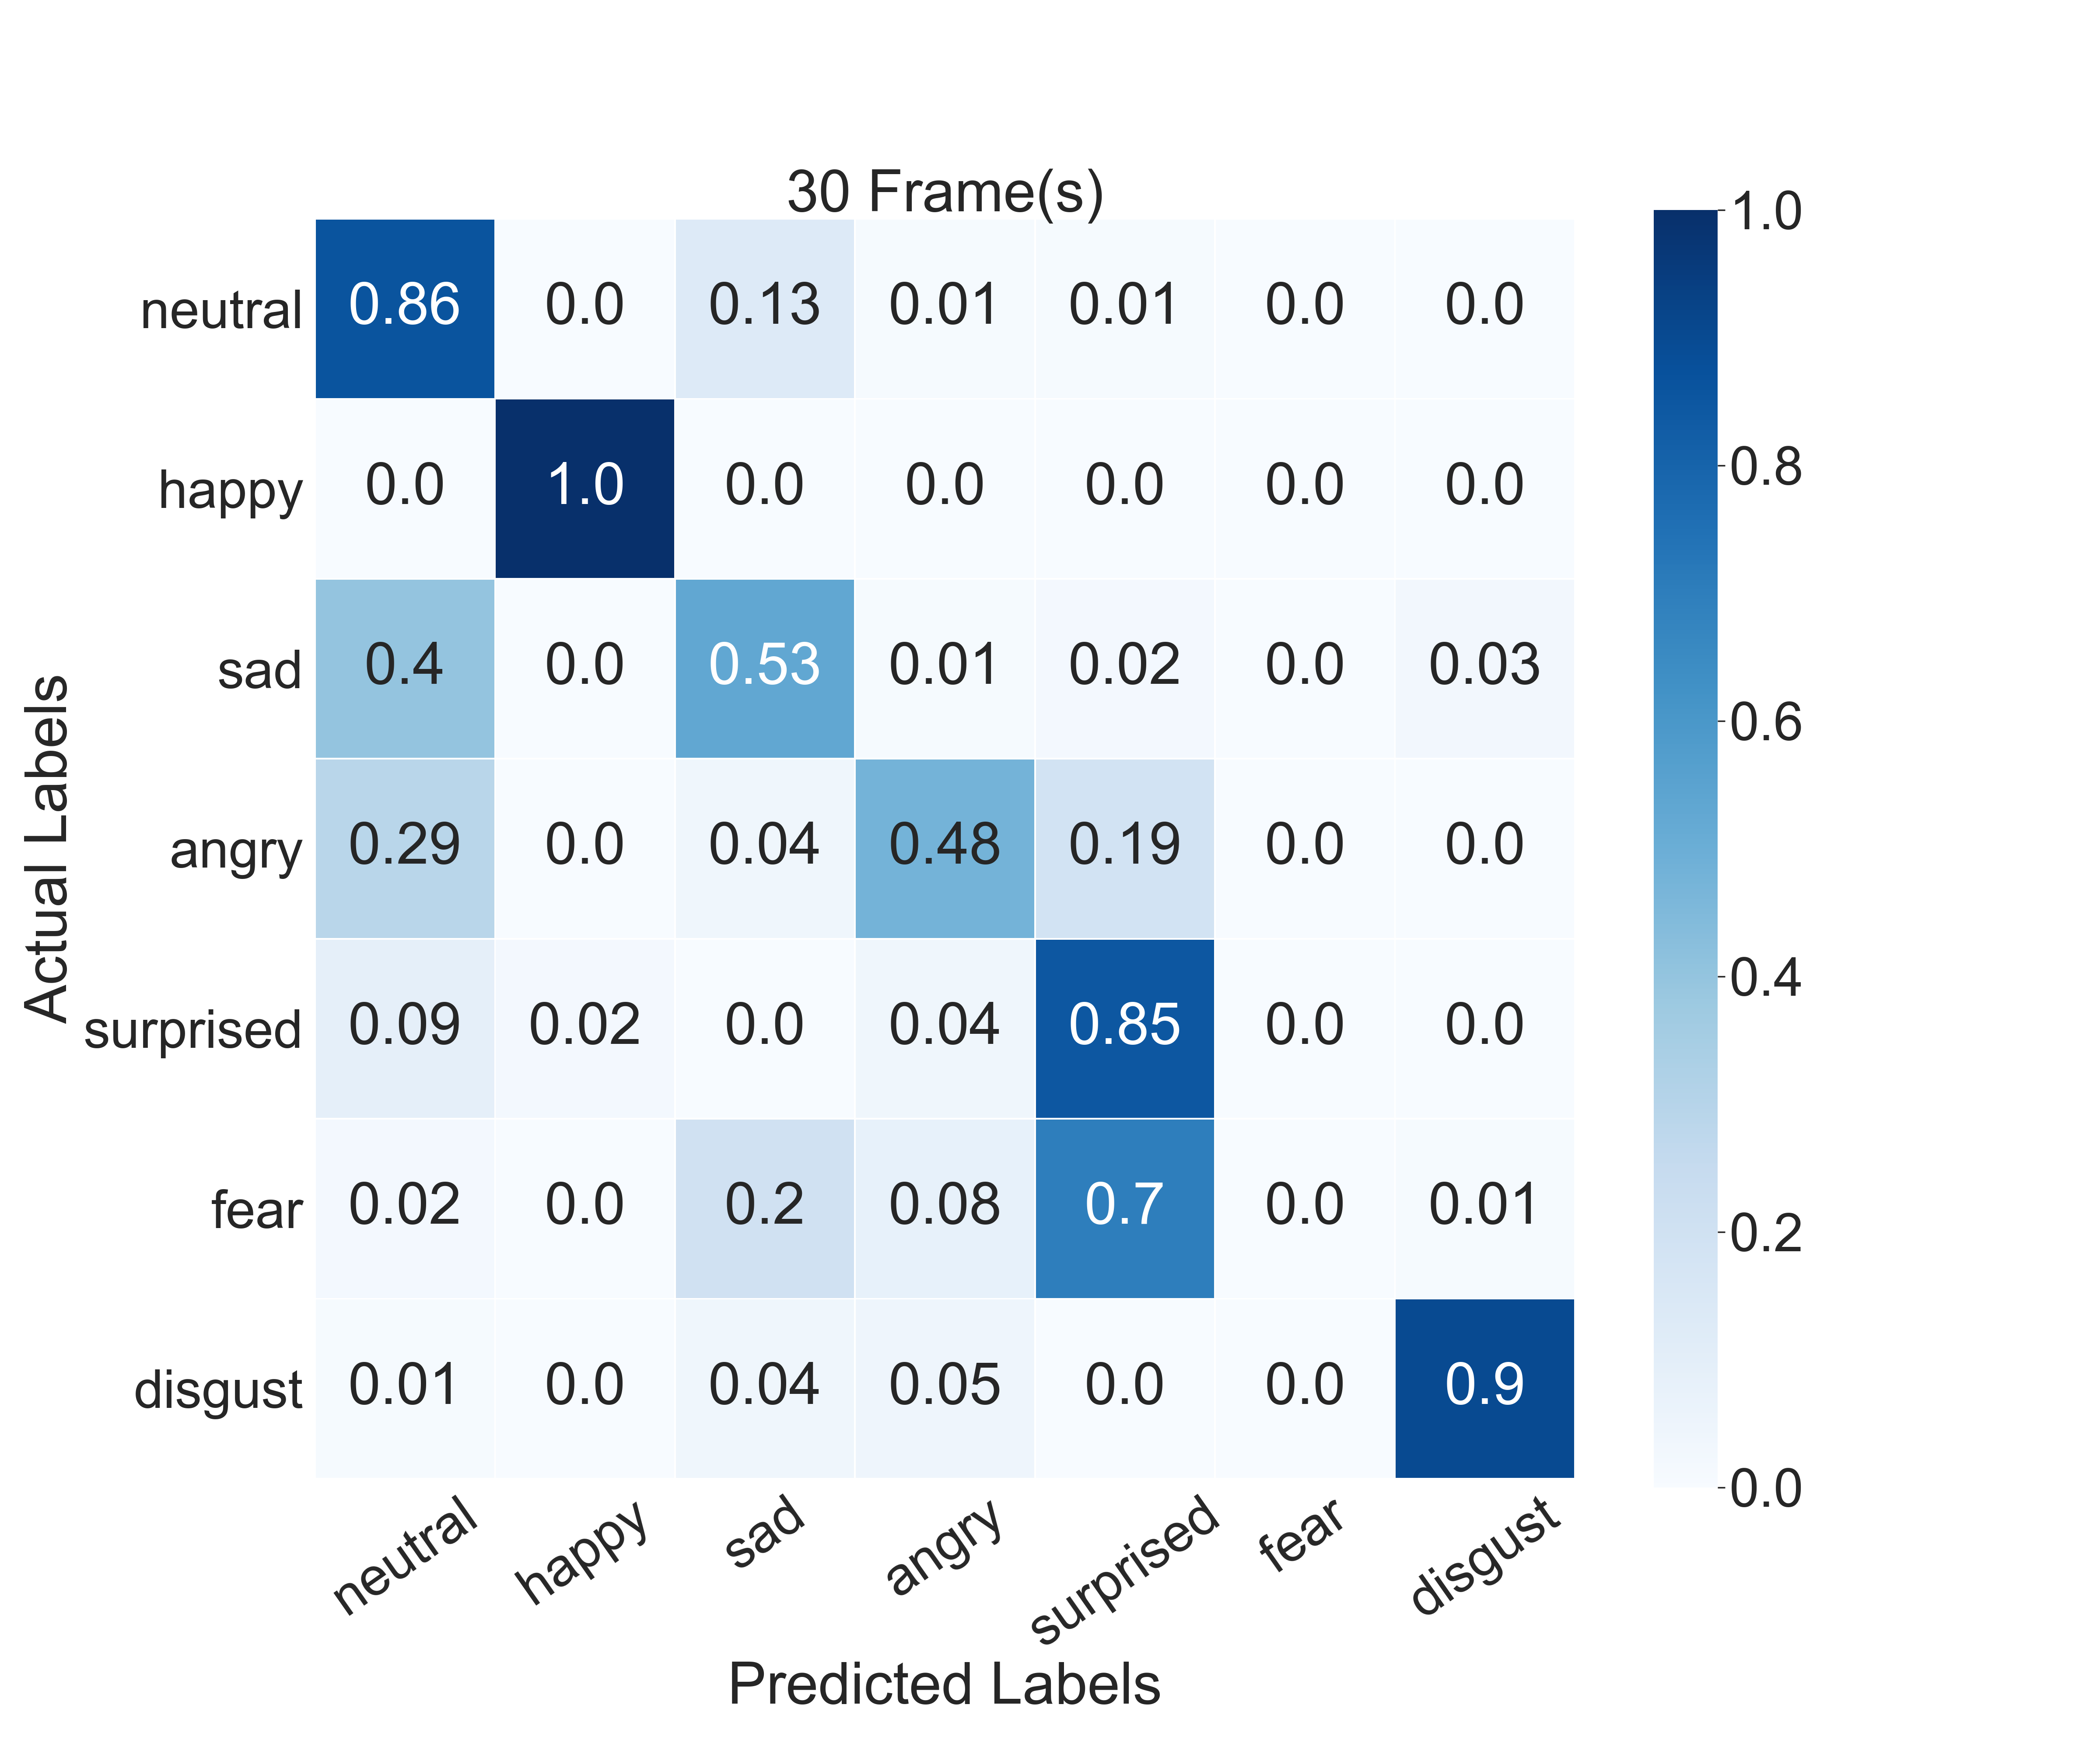
\includegraphics[width=\textwidth]{res/conf_fusion_30.png}
    \end{subfigure}
    \begin{subfigure}[b]{0.45\textwidth}
      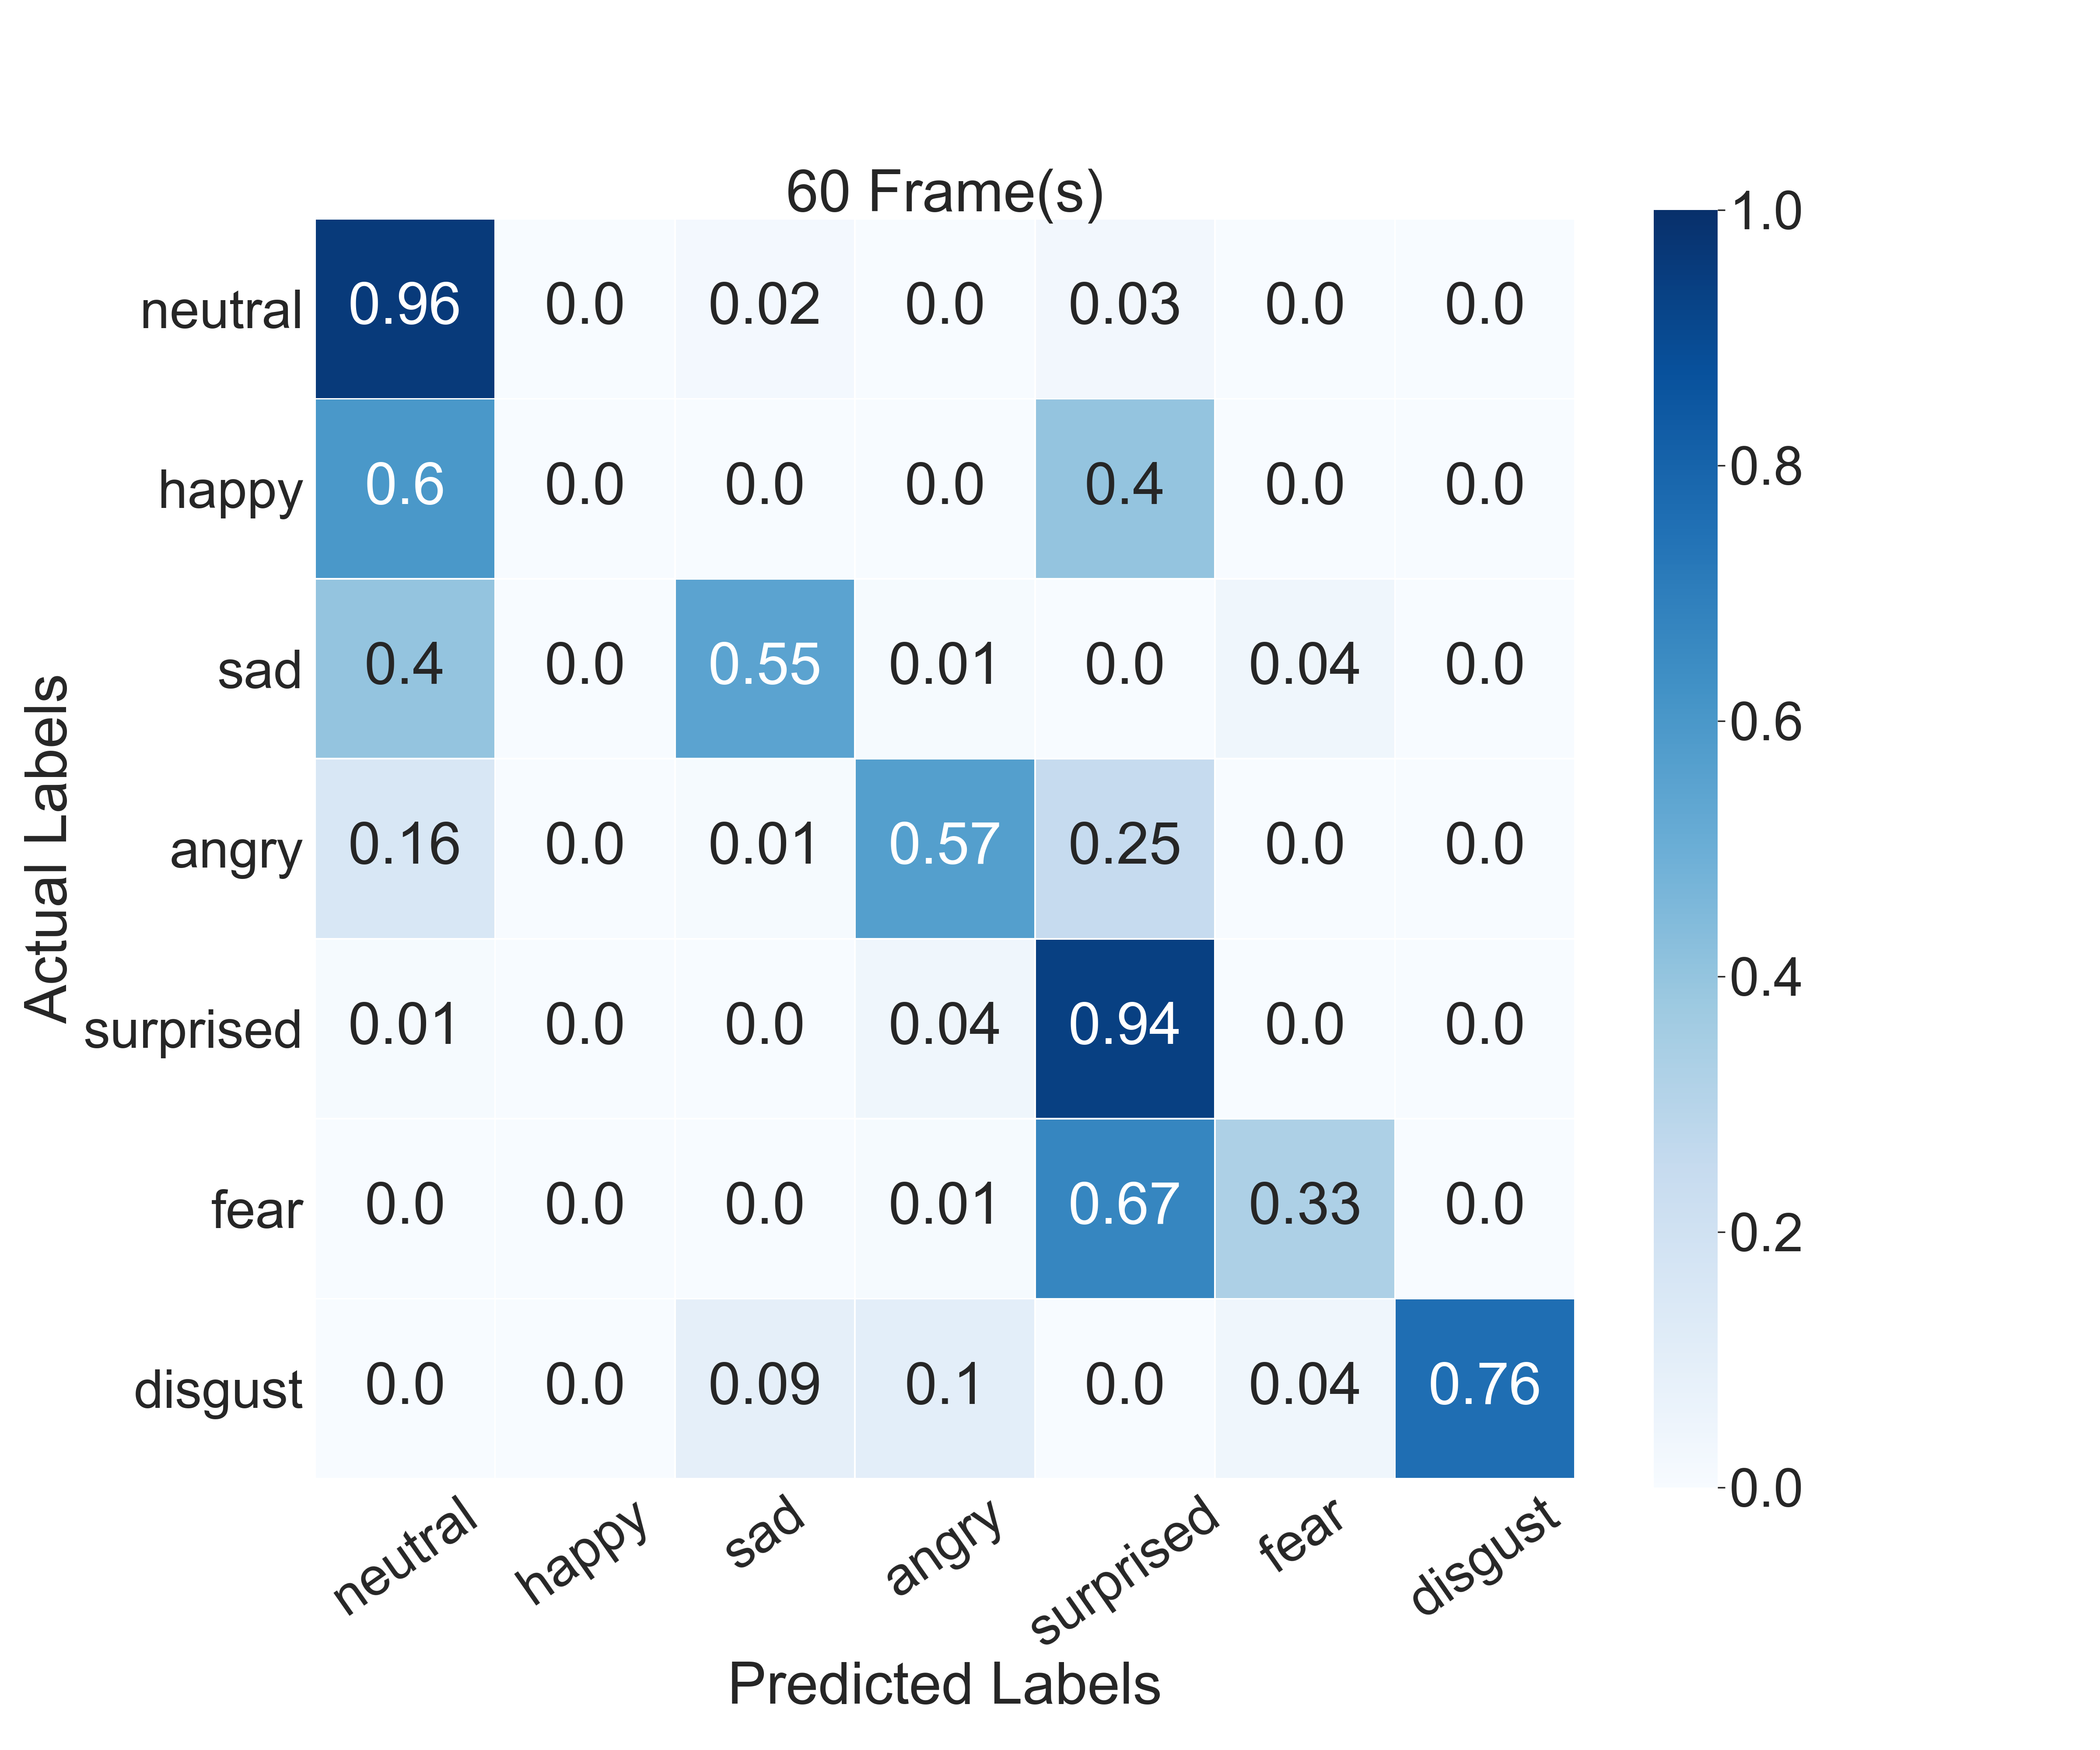
\includegraphics[width=\textwidth]{res/conf_fusion_60.png}
    \end{subfigure}
    \begin{subfigure}[b]{0.45\textwidth}
      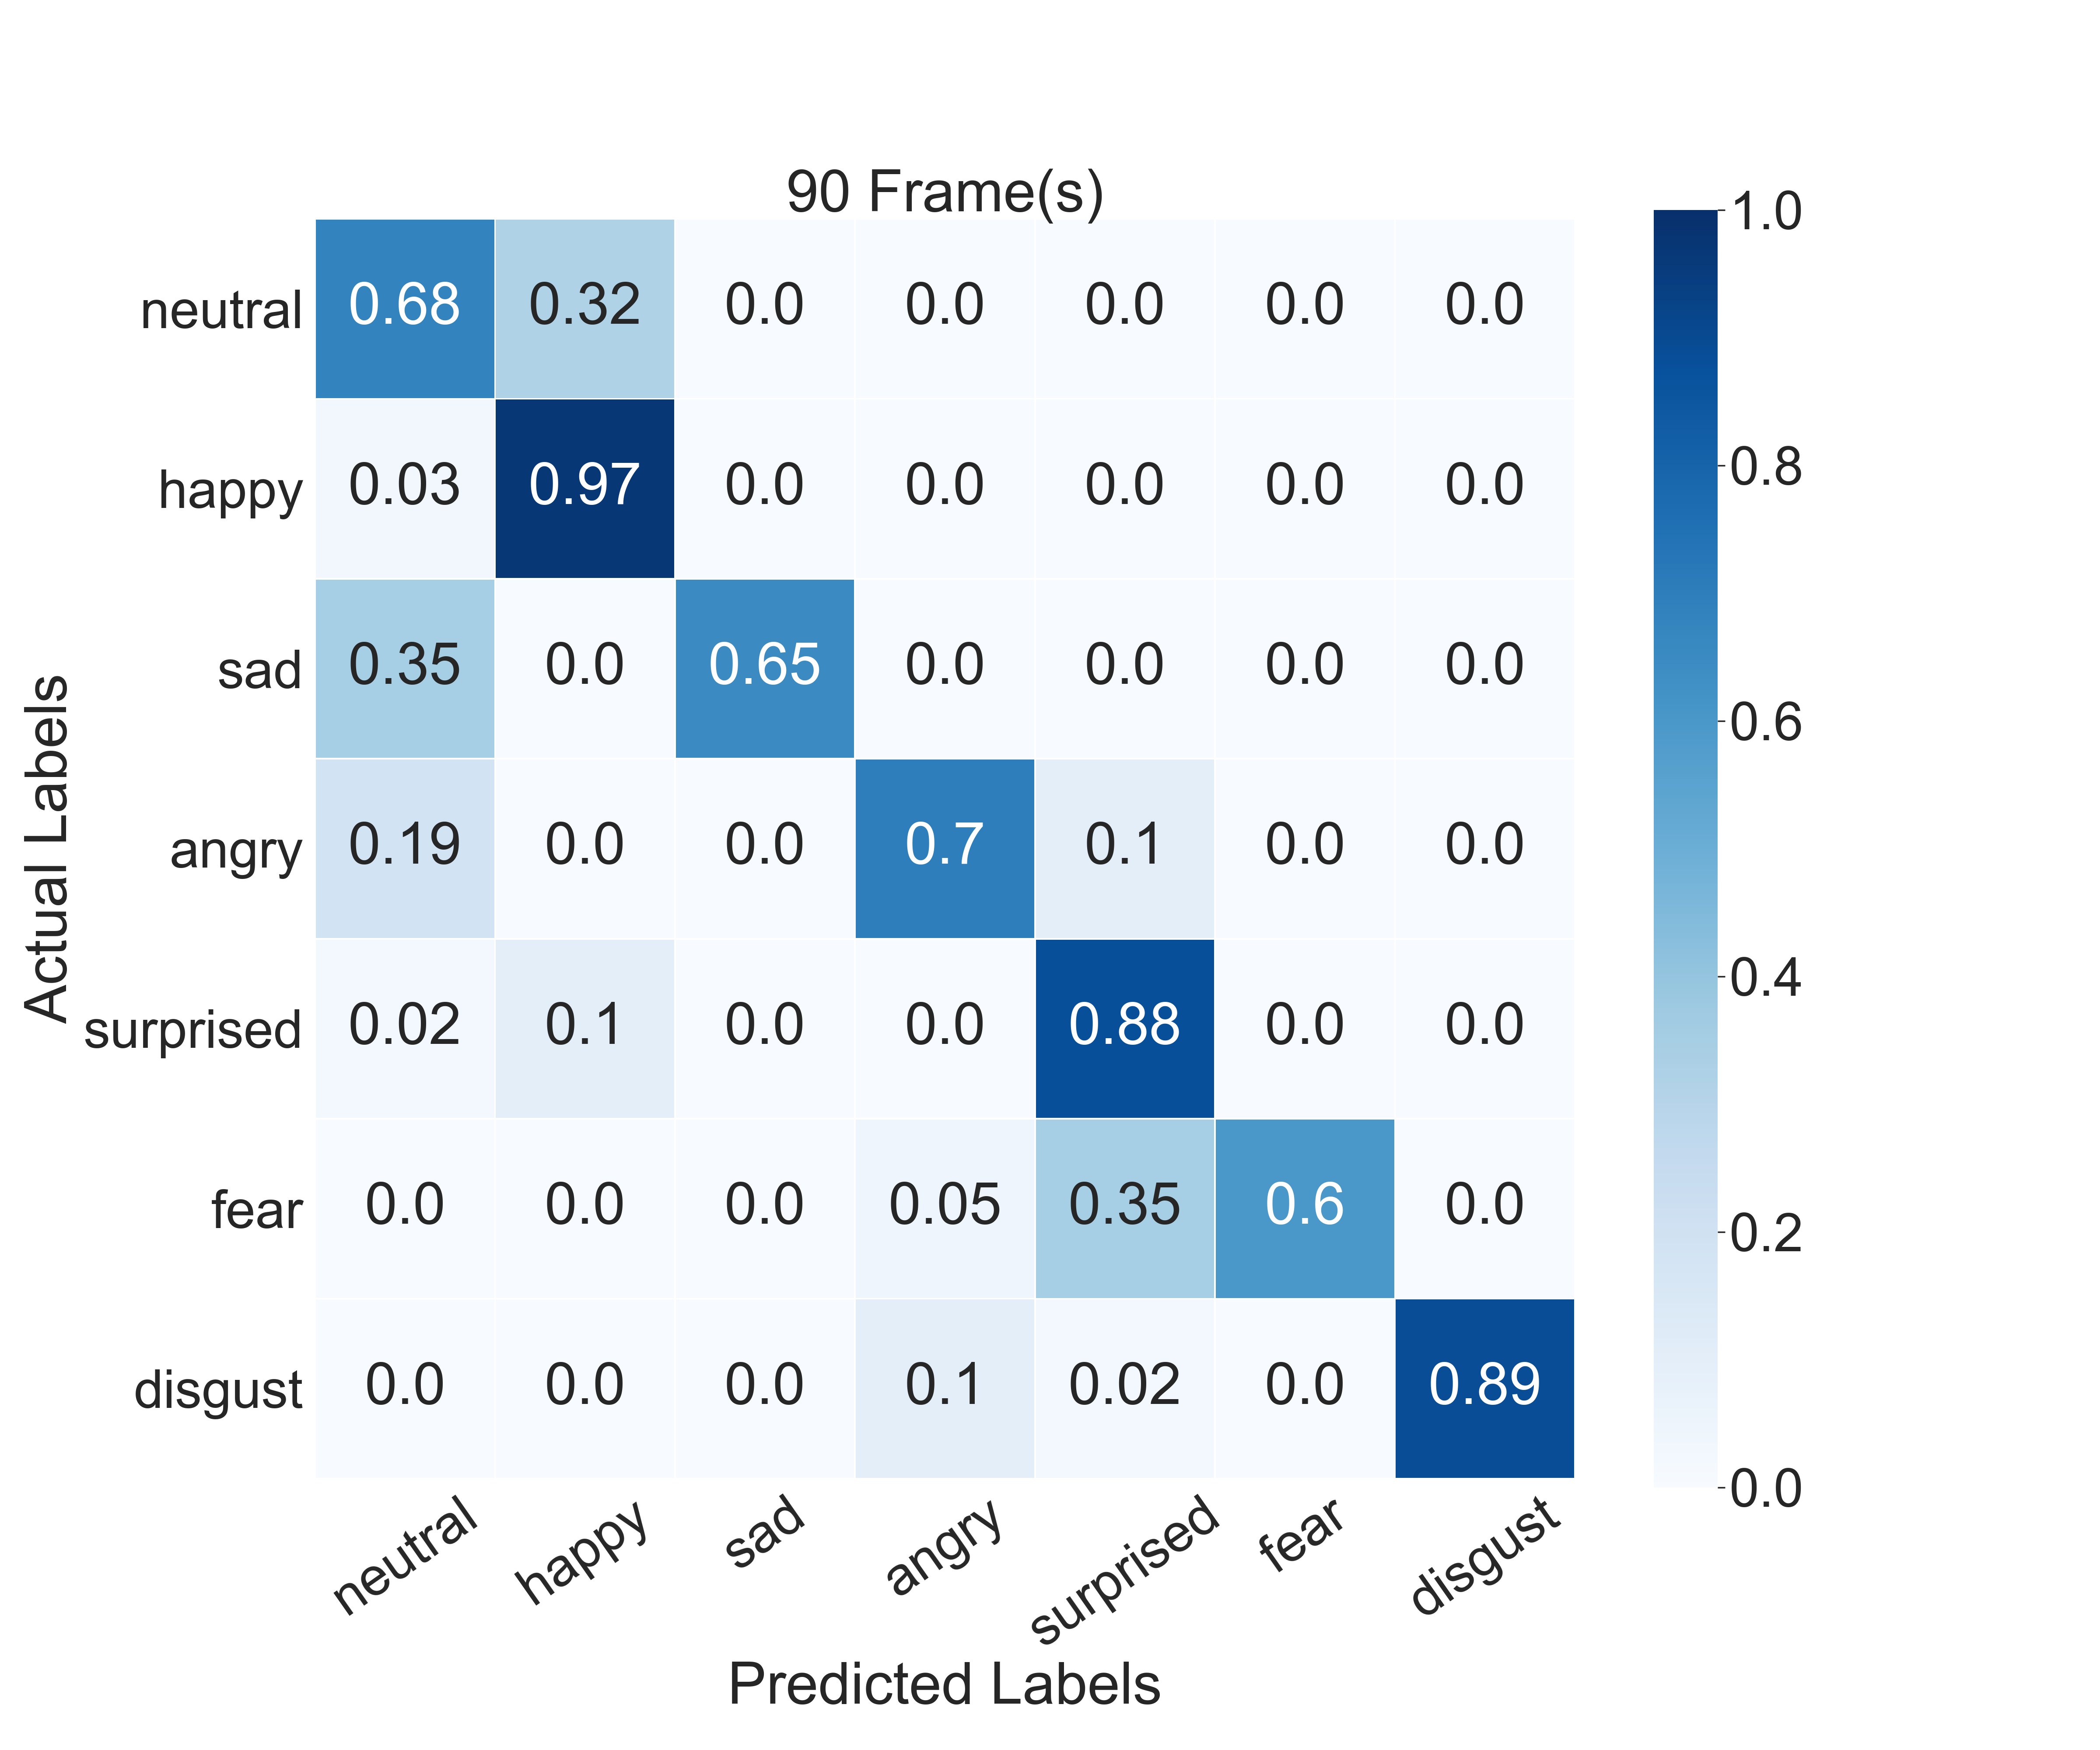
\includegraphics[width=\textwidth]{res/conf_fusion_90.png}
    \end{subfigure}
    \caption{Confusion matrices of the validation data for the LipNet fusion model (FER-LN).}
    \label{fig:lipnet_conf}
\end{figure}
\begin{figure}
    \centering
    \begin{subfigure}[b]{0.45\textwidth}
      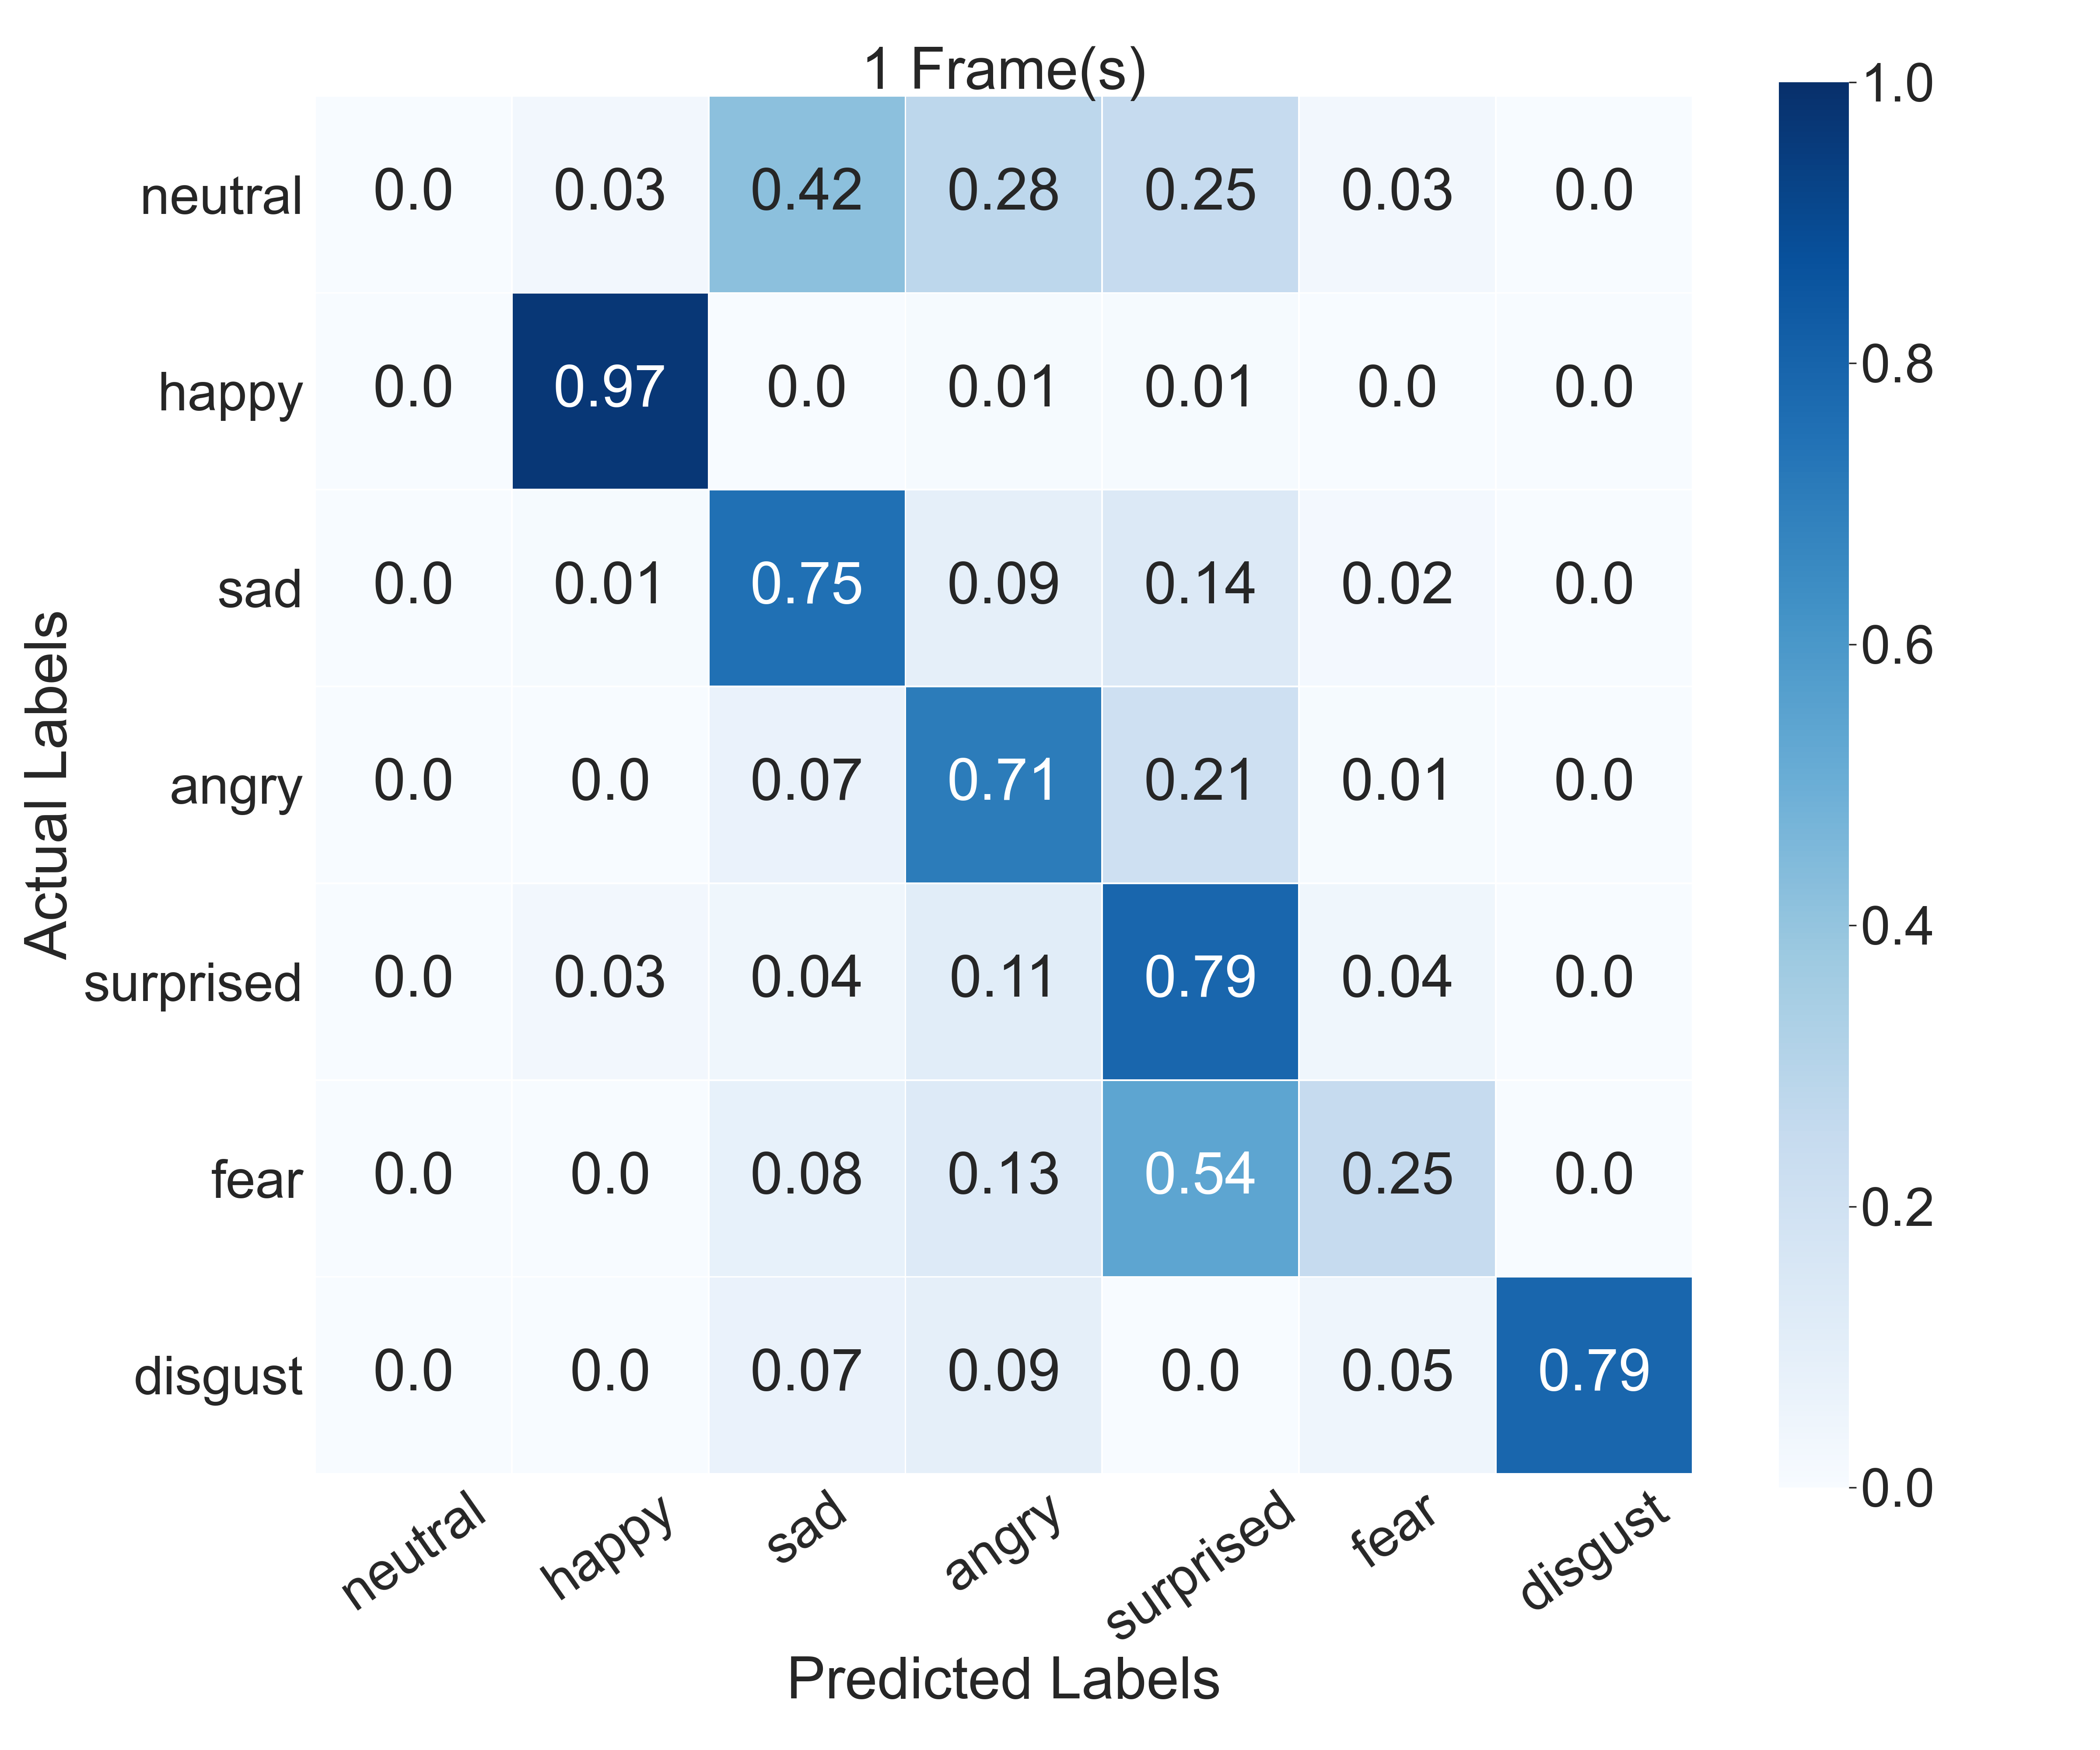
\includegraphics[width=\textwidth]{res/conf_busso_1.png}
    \end{subfigure}
    \begin{subfigure}[b]{0.45\textwidth}
      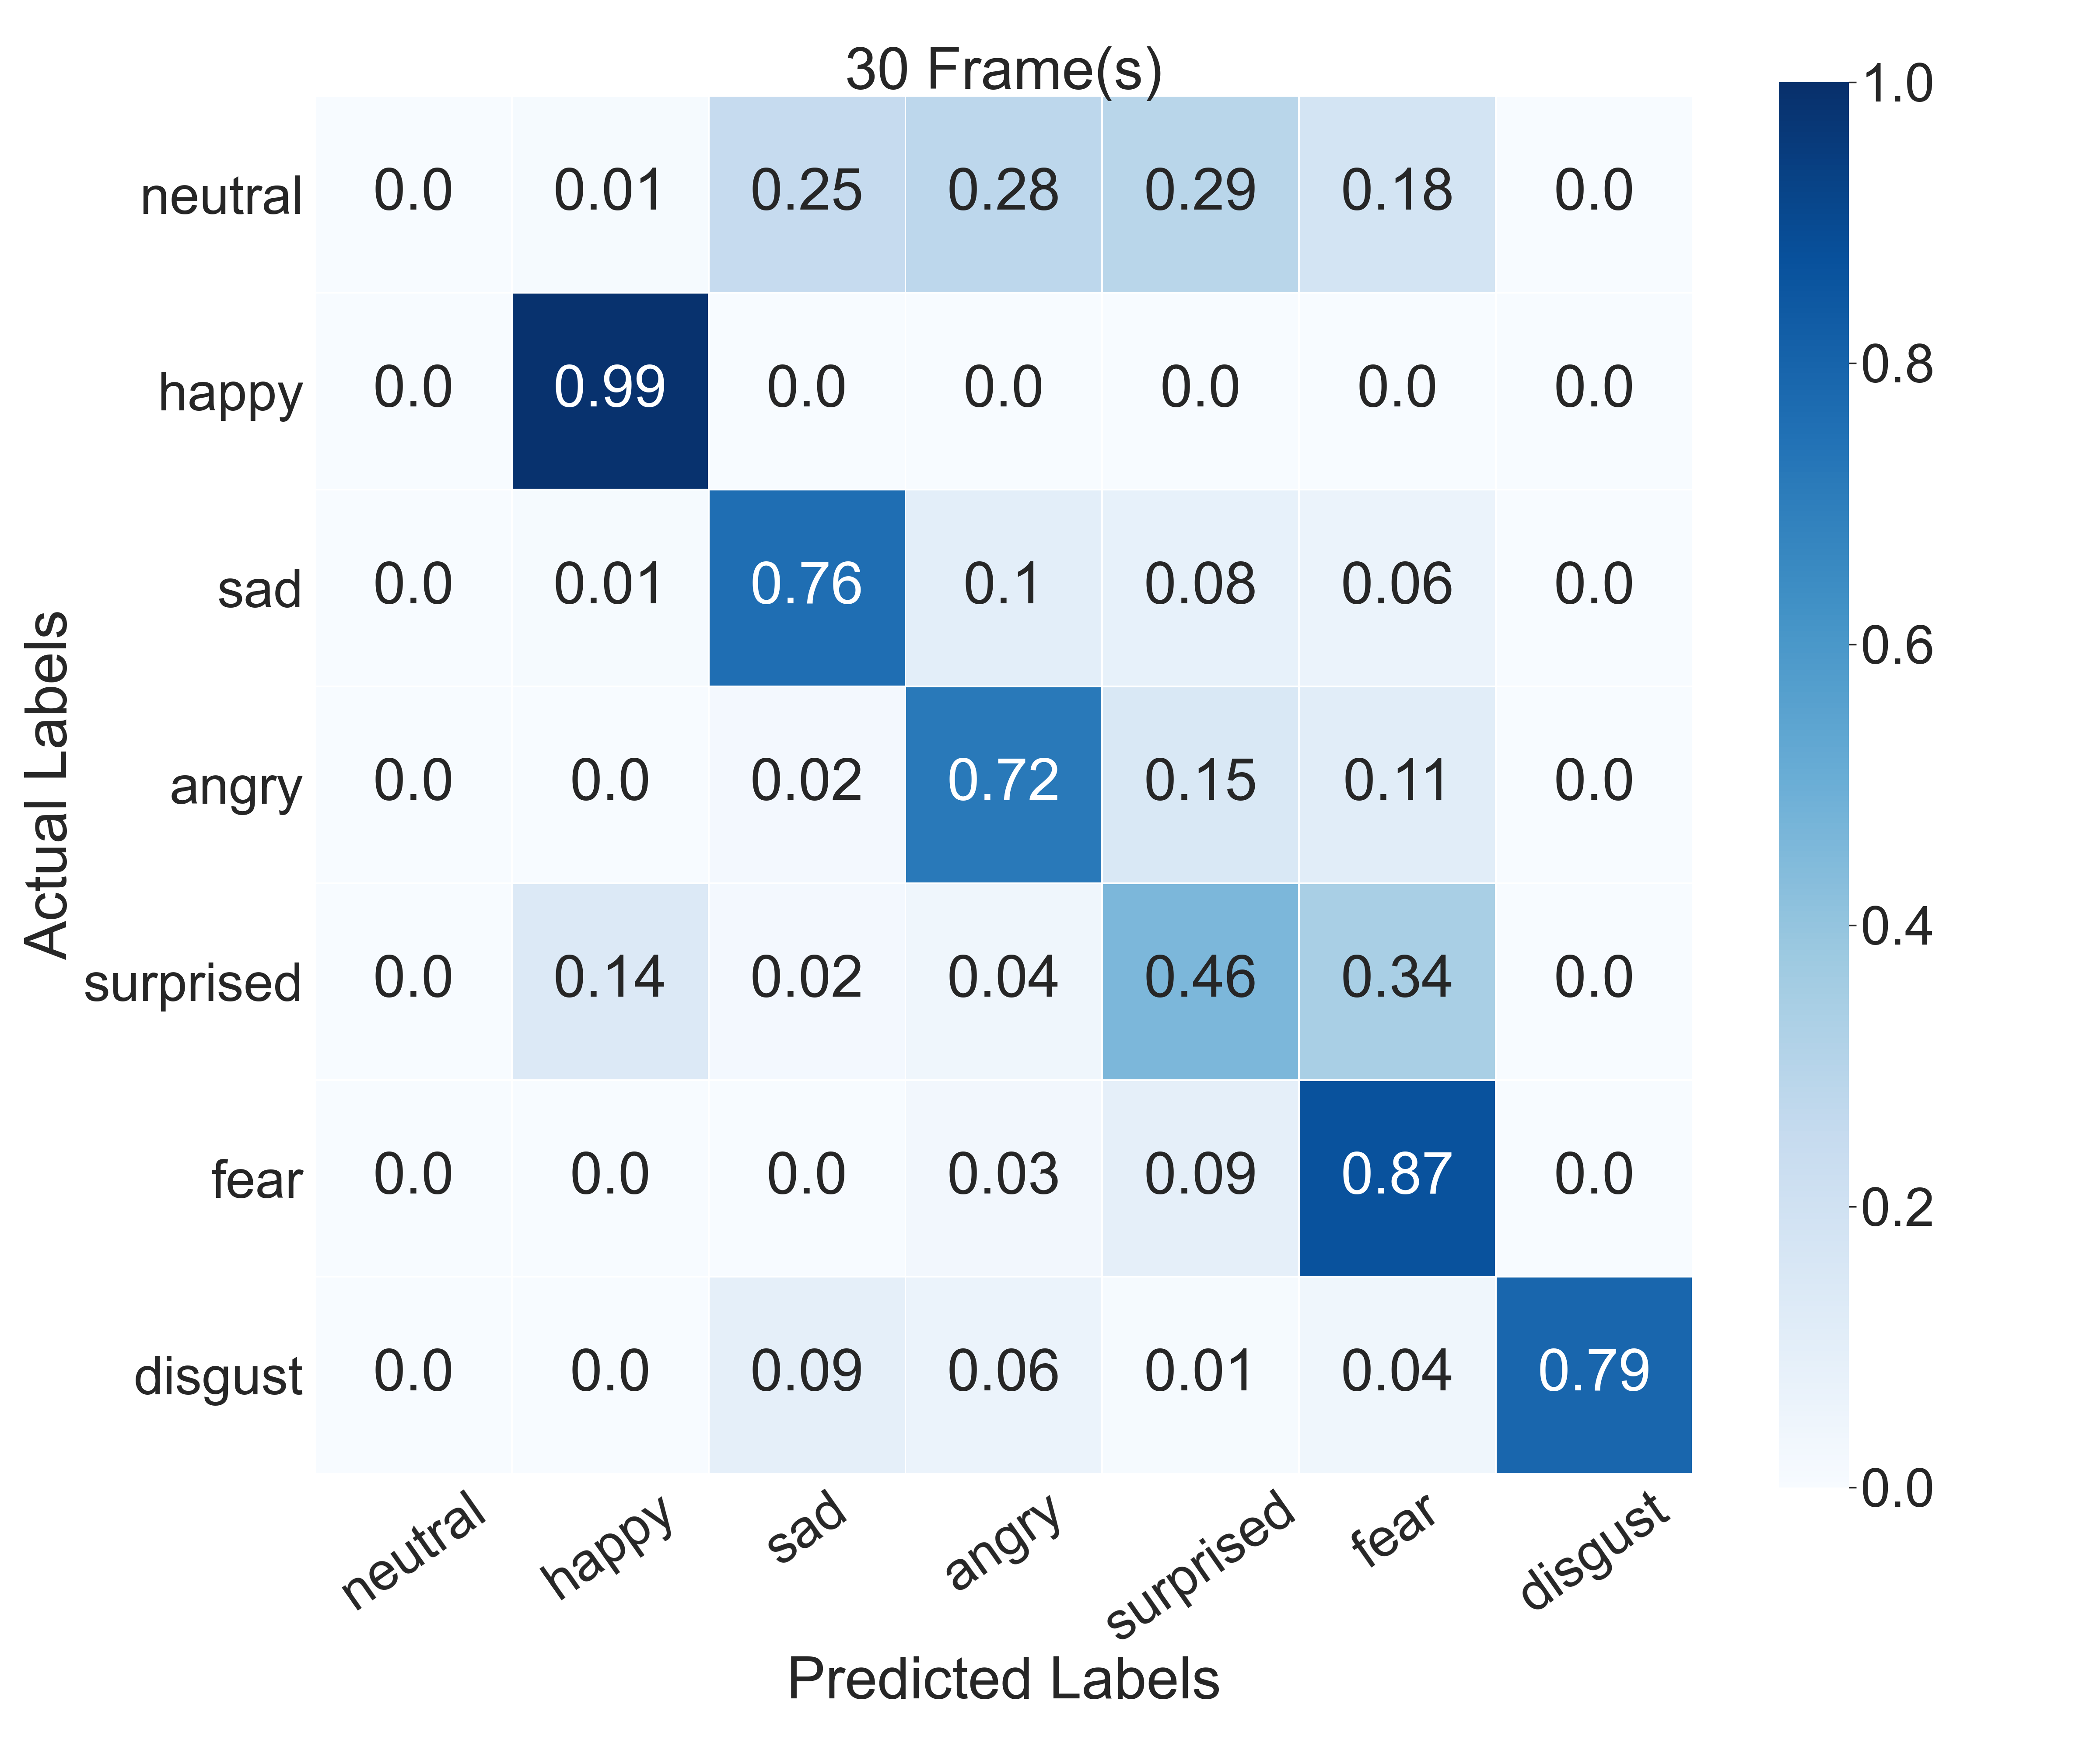
\includegraphics[width=\textwidth]{res/conf_busso_30.png}
    \end{subfigure}
    \begin{subfigure}[b]{0.45\textwidth}
      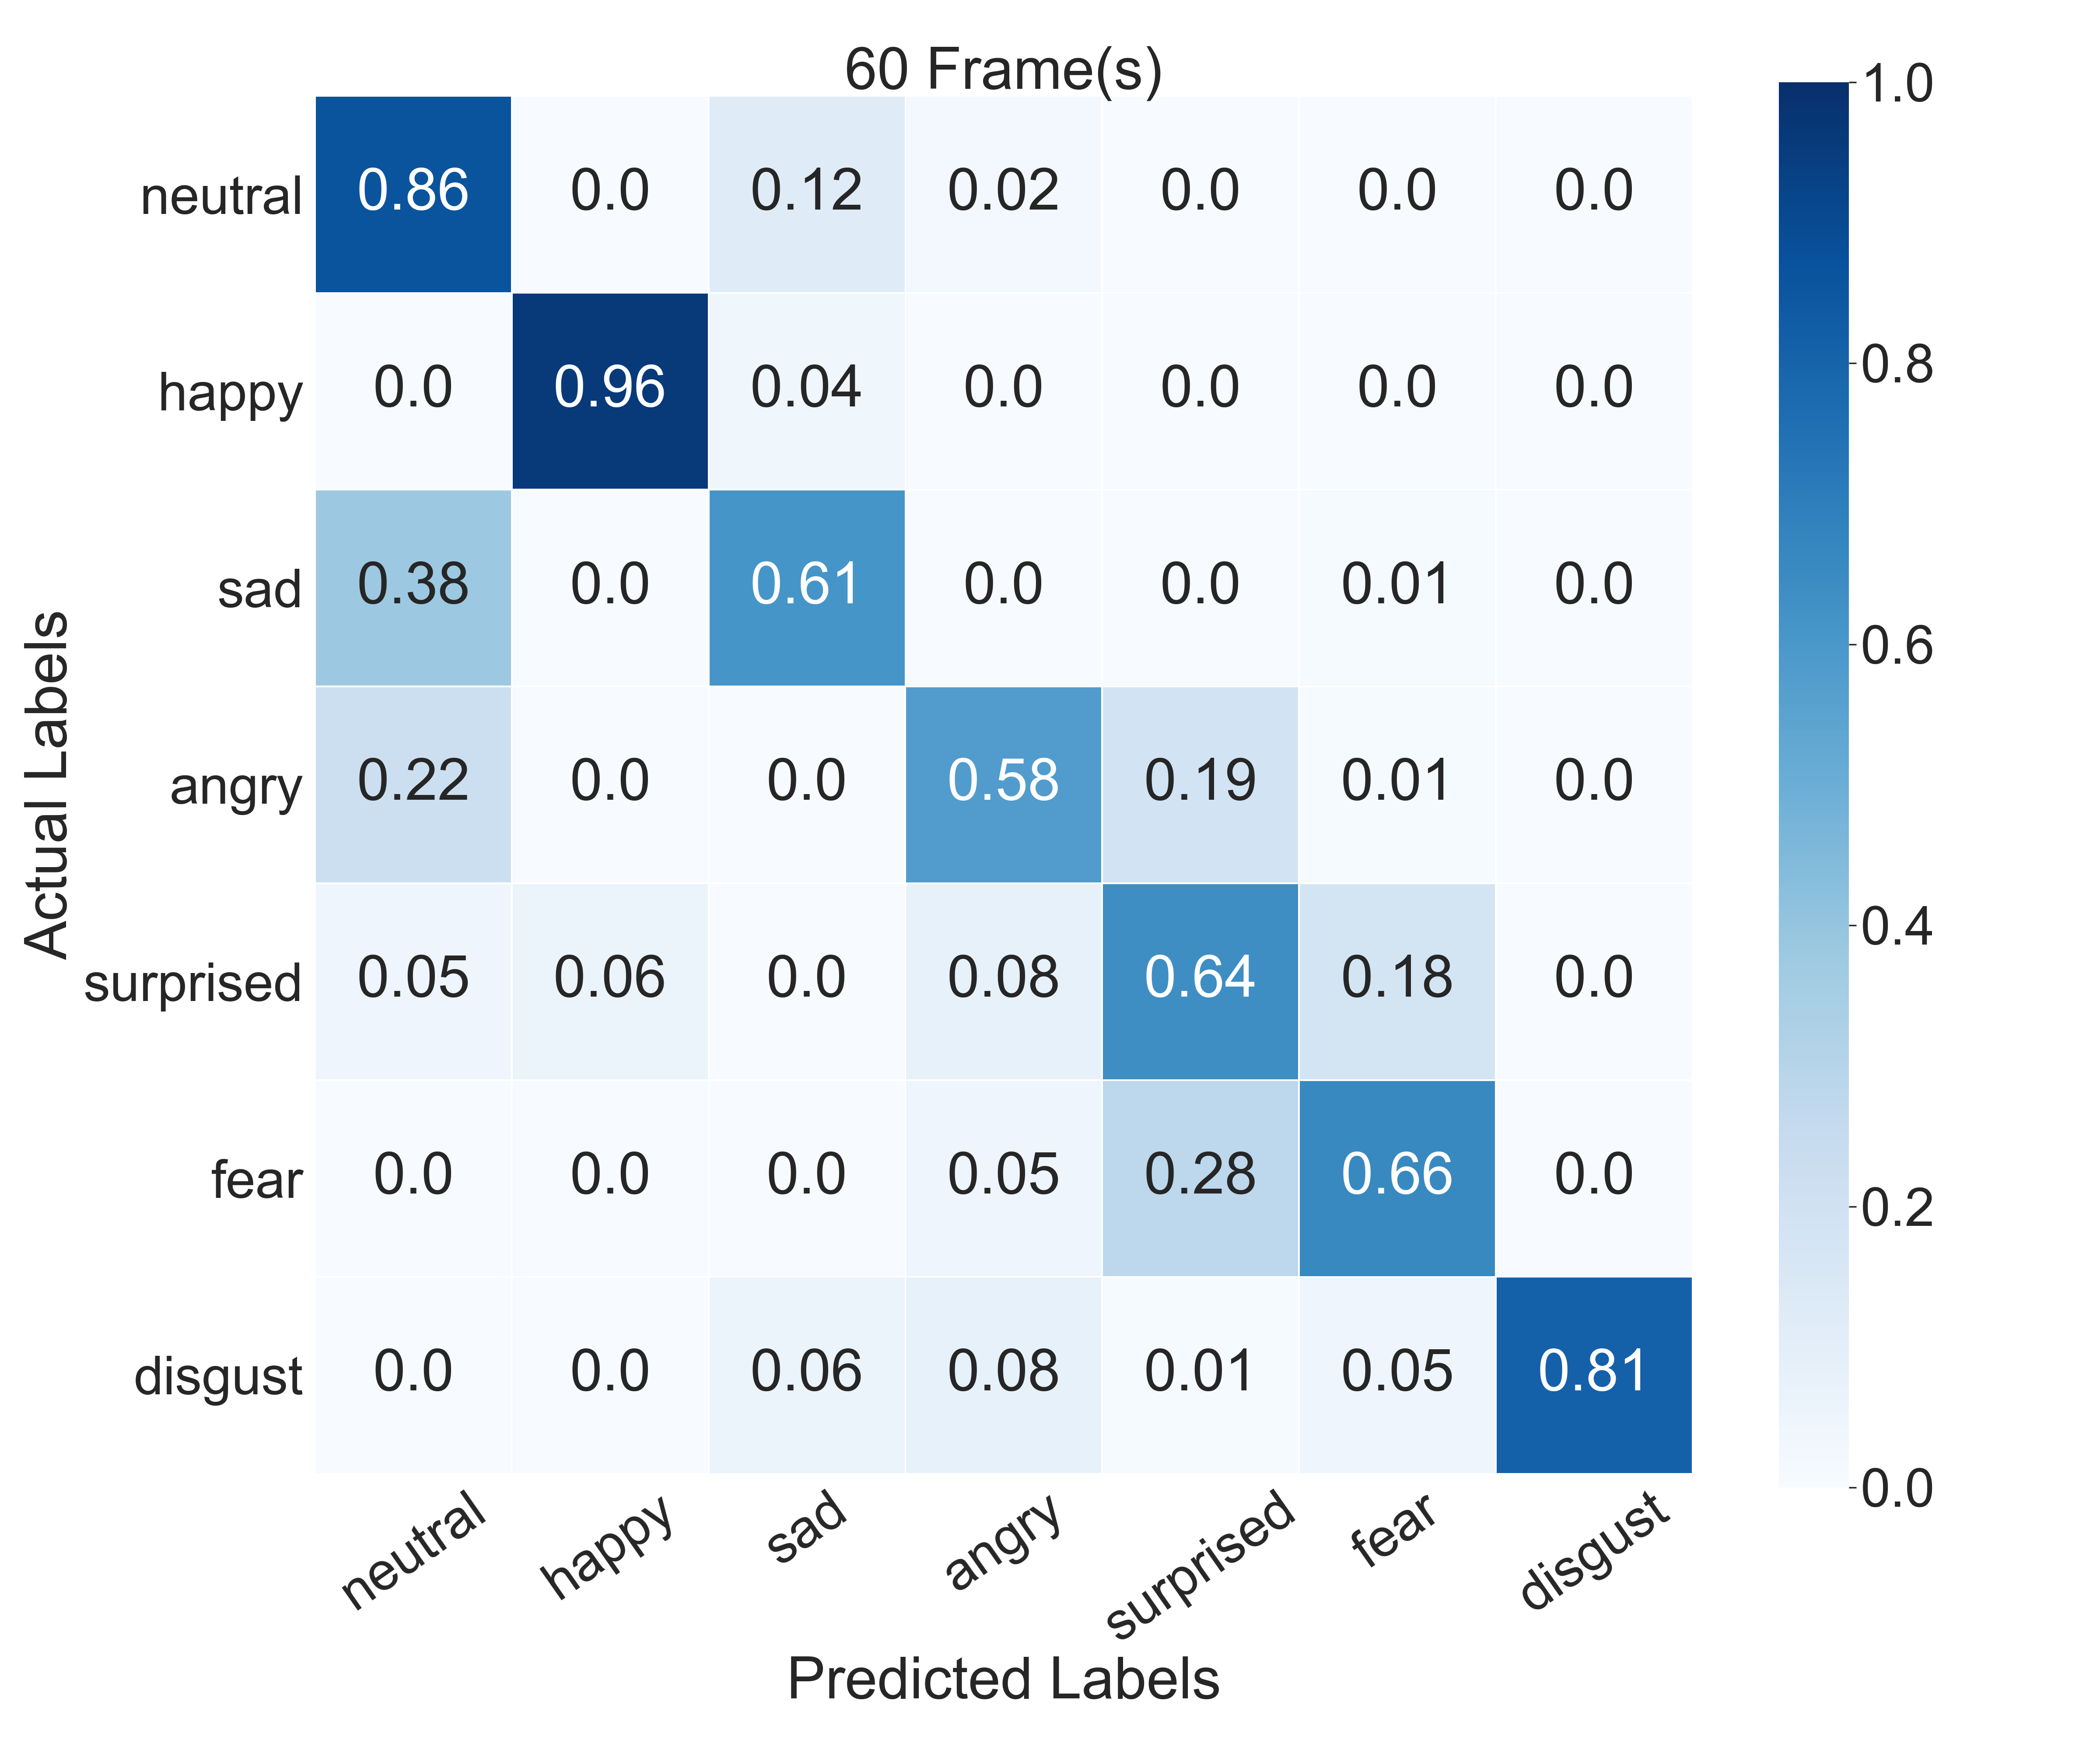
\includegraphics[width=\textwidth]{res/conf_busso_60.png}
    \end{subfigure}
    \begin{subfigure}[b]{0.45\textwidth}
      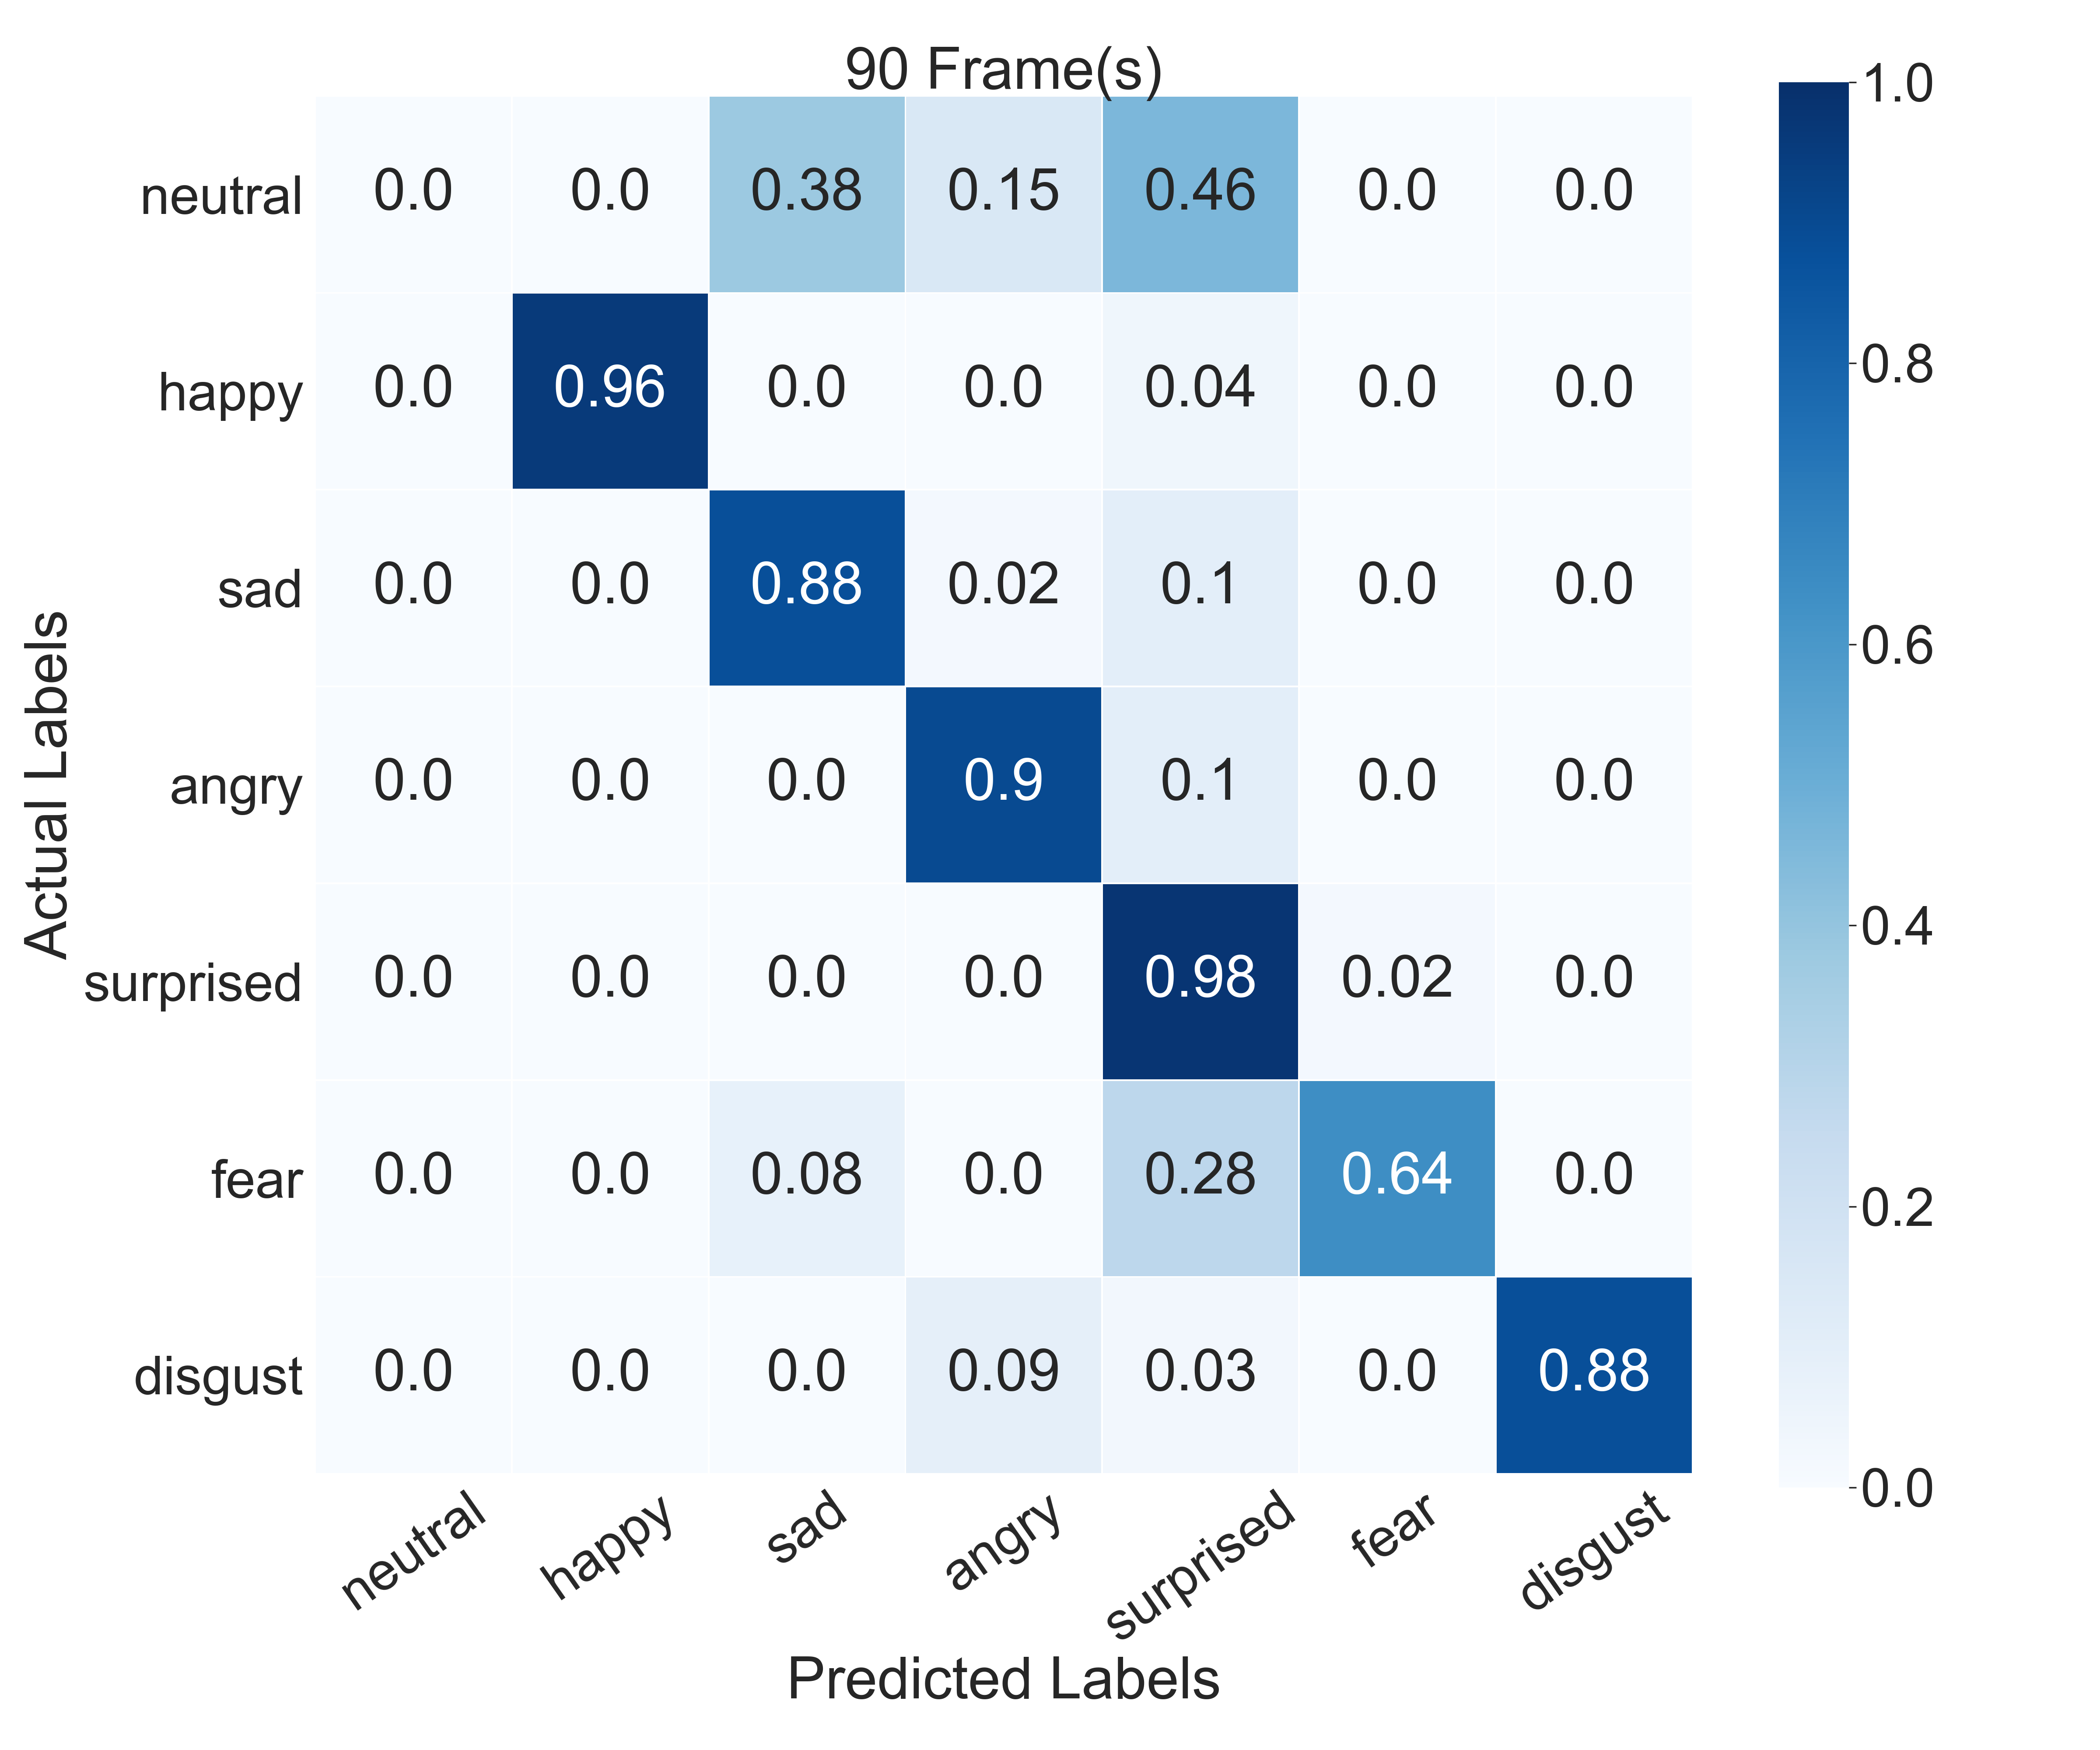
\includegraphics[width=\textwidth]{res/conf_busso_90.png}
    \end{subfigure}
    \caption{Confusion matrices of the validation data for the Style Extractor fusion model (FER-SE).}
    \label{fig:busso_conf}
\end{figure}


Confusion matrices allow us to take a deeper look into the model performance. Figure \ref{fig:fer_conf} shows the confusion matrices of the FER-TC model through all frame-window sizes. We notice a consistent overfitting towards \texttt{neutral} labels in all temporal settings. There also remain significant mislabels around \texttt{surprised} labels on models with 1, 30, and 60 frames. At 90 frames, the model becomes very robust on all other emotions except for the overfitting towards \texttt{neutral}.

The confusion matrices for the FER-LN model in figure \ref{fig:lipnet_conf} similarly show an improvement along the temporal dimension. A similar overfit towards \texttt{neutral} persists throughout. However at 90 frames, the FER-LN model does not manage to alleviate the issues surrounding false \texttt{surprised} labels. The overfit on \texttt{surprised} was indeed lower on the single frame model. This might however be explained by the very severe overlabelling on \texttt{neutral} labels in that model.

A different pattern emerges on the model using our own style extractor in figure \ref{fig:busso_conf}. The \texttt{neutral} label is ignored by the model, except when trained on 60 frames. The \texttt{surprised} emotion has a notably worse performance compared to the other emotions, which can be explained by the lack of surprised videos in the CREMA-D dataset used to train the style extractor. \texttt{Happy} stands out as an emotion that is particularly robust and stable, neither having many false positives nor false negatives. 

The underfitting on the \texttt{neutral} emotion might point to design issues on the style extractor. It was trained purely with the intention of transforming emotional meshes to neutral counterparts. The neutral-to-neutral transformation, which should not morph the input at all, was ignored.

There are no significant differences on emotional performance on either the FER-TC or the FER-LN model. They struggle across the same classes (\texttt{sad}, \texttt{angry}) and have better performance on \texttt{happy} and \texttt{surprised}. This is notably different on the FER-SE model. The emotions of \texttt{sad} and \texttt{angry} perform significantly better on all frame-window sizes except 60. This is also the frame-window size at which the \texttt{neutral} emotion does not underfit, which might be the reason for this shift in accuracy. At 60 frames, a significant mislabelling of \texttt{sad} and \texttt{angry} data is classified as \texttt{neutral}, as with the other models.

Figure \ref{fig:rd_intensity} shows the accuracy on the validation data split by intensity level. The RAVDESS corpus splits the intensity of the recordings into \texttt{normal} and \texttt{high} intensity. Recordings in the \texttt{neutral} emotion are always of \texttt{normal} intensity. We can see that higher intensity videos are labelled more accurately than those of \texttt{normal} intensity. The FER-SE model becomes more robust in regards to intensity as the frame-window size increases, reducing the difference between \texttt{normal} and \texttt{high} intensities from 17 to seven percentage points. The FER-TC model follows a similar trend, decreasing the split from eleven to three percentage points from a frame-window size of 1 to 60. At 90 frames however the difference hits its peak at 18 percentage points. The difference between \texttt{normal} and \texttt{high} intensities stays at comparable levels throughout all frame-window sizes for the FER-LN model. The very high performance of the FER-LN model on 60 and 90 frame-window sizes on \texttt{high} intensity is particularly interesting. Exaggerated motions in the \texttt{high} intensity videos of RAVDESS in the orofacial area are beneficial for the FER-LN model, which takes parts of its input from that region of the face. Another point of note is the performance of the FER-SE model on \texttt{normal} intensities. The FER-SE model struggles on \texttt{neutral} emotions. With all \texttt{neutral} videos also being of \texttt{normal} intensity, the results might be skewed. When looking at figure \ref{fig:busso_no_normal}, we can see the differences between \texttt{normal} and \texttt{high} intensities for the FER-SE model for all frame-window sizes when we ignore the \texttt{neutral} emotion. Here we can see more robust performance on the intensity split, except for a frame-window size of 60. This is the frame-window size where the model does not underfit on the \texttt{neutral} emotion.
We will discuss the difference in intensity levels again in section \ref{sec:cross_dataset}, where we will do a similar analysis on the CREMA-D corpus.

Given the results of the models using a lexical compensator, the FER-LN model does not perform as well as the FER-SE model on validation data. Section \ref{sec:cross_dataset} will go into more detail of model performance across different datasets. Considering the simple nature of our style extractor, a more refined version of it, trained on more diverse data, could achieve even better results.
% TODO: epochs -> best result after 4-7 epochs
\begin{figure}
    \centering
    \begin{subfigure}[b]{0.45\textwidth}
      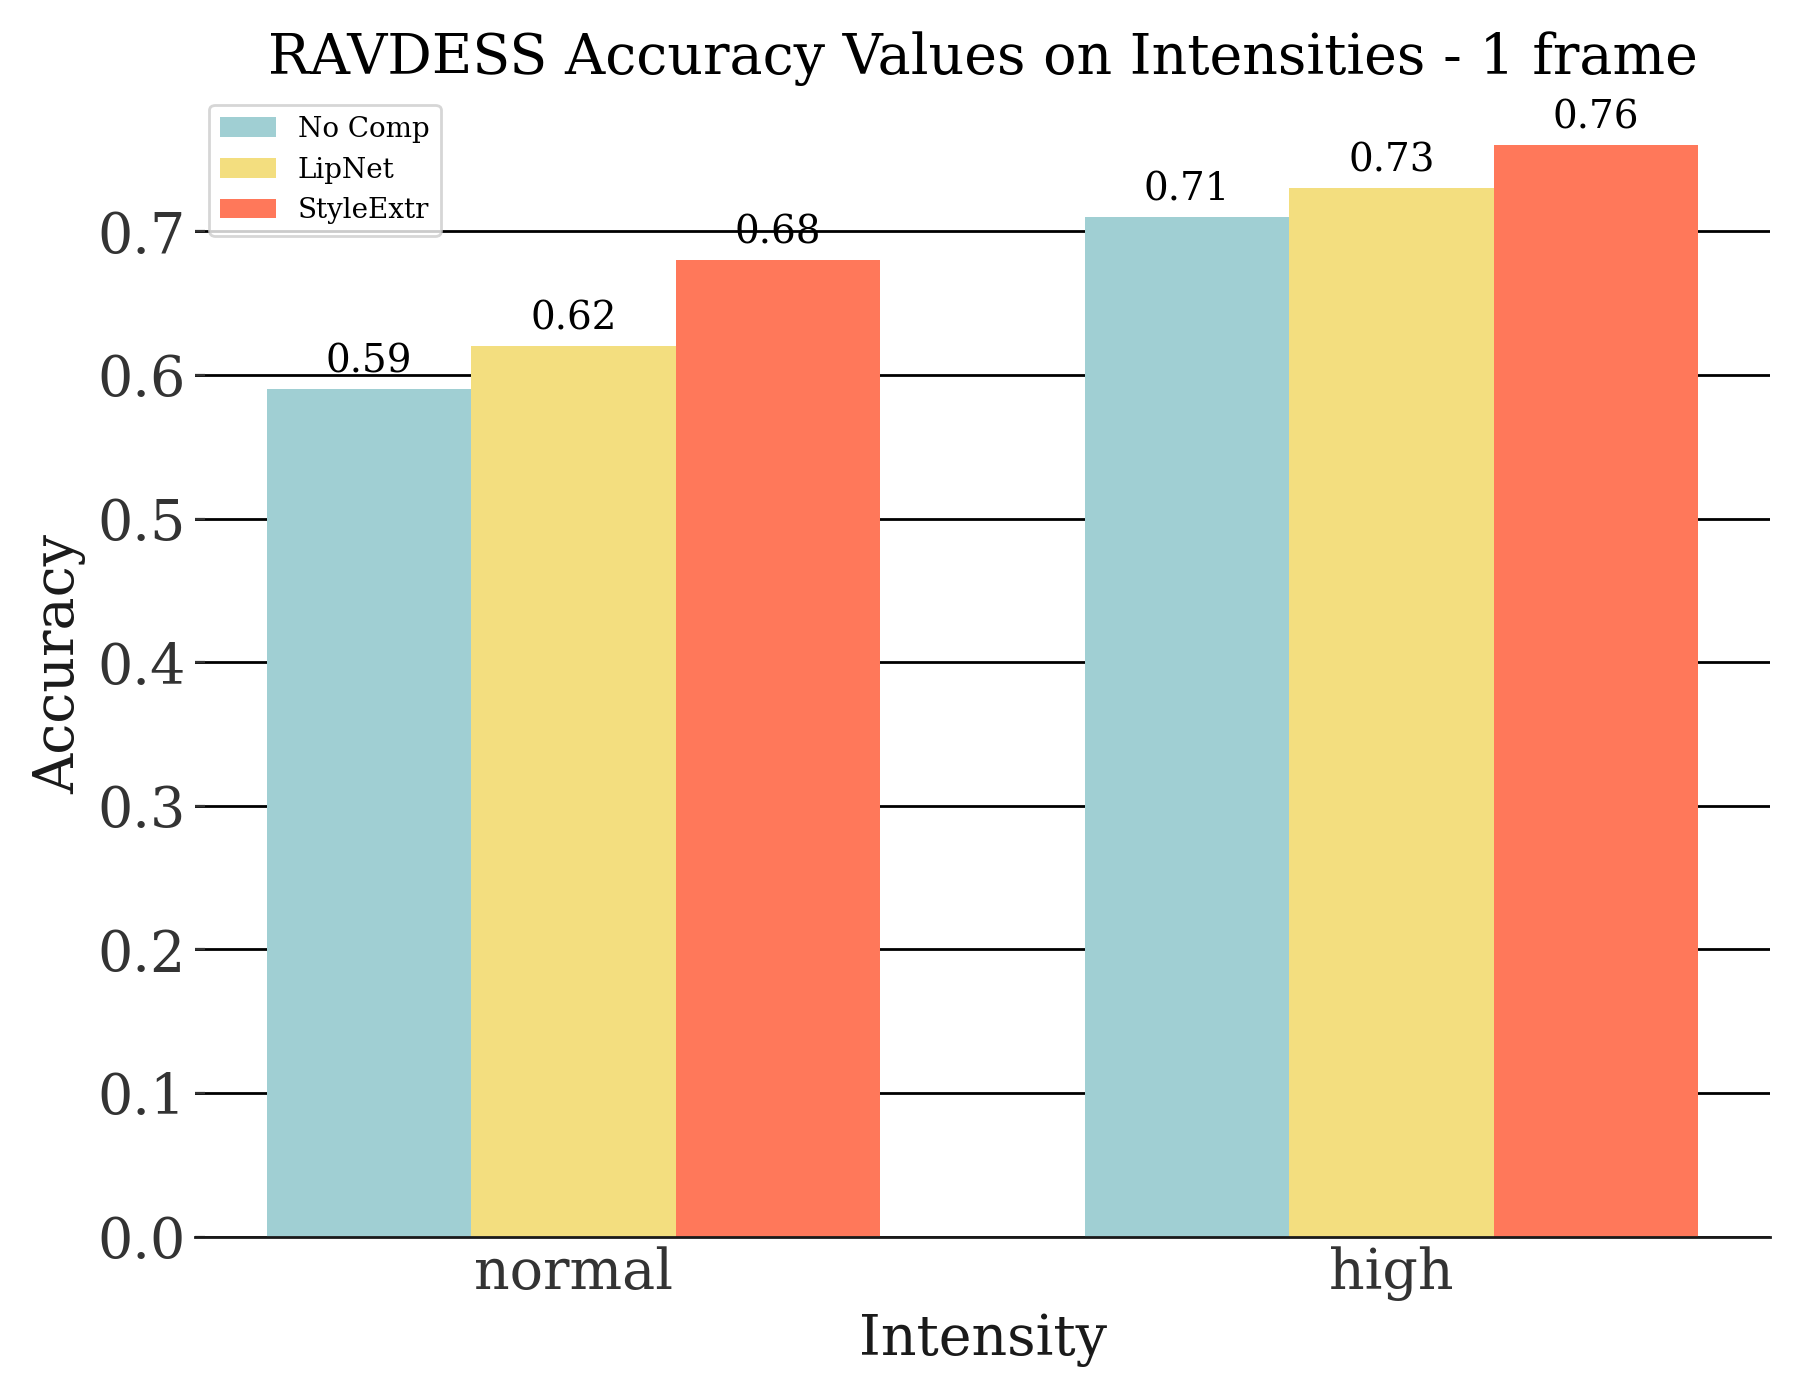
\includegraphics[width=\textwidth]{res/rd-intensities-1.png}
    \end{subfigure}
    \begin{subfigure}[b]{0.45\textwidth}
      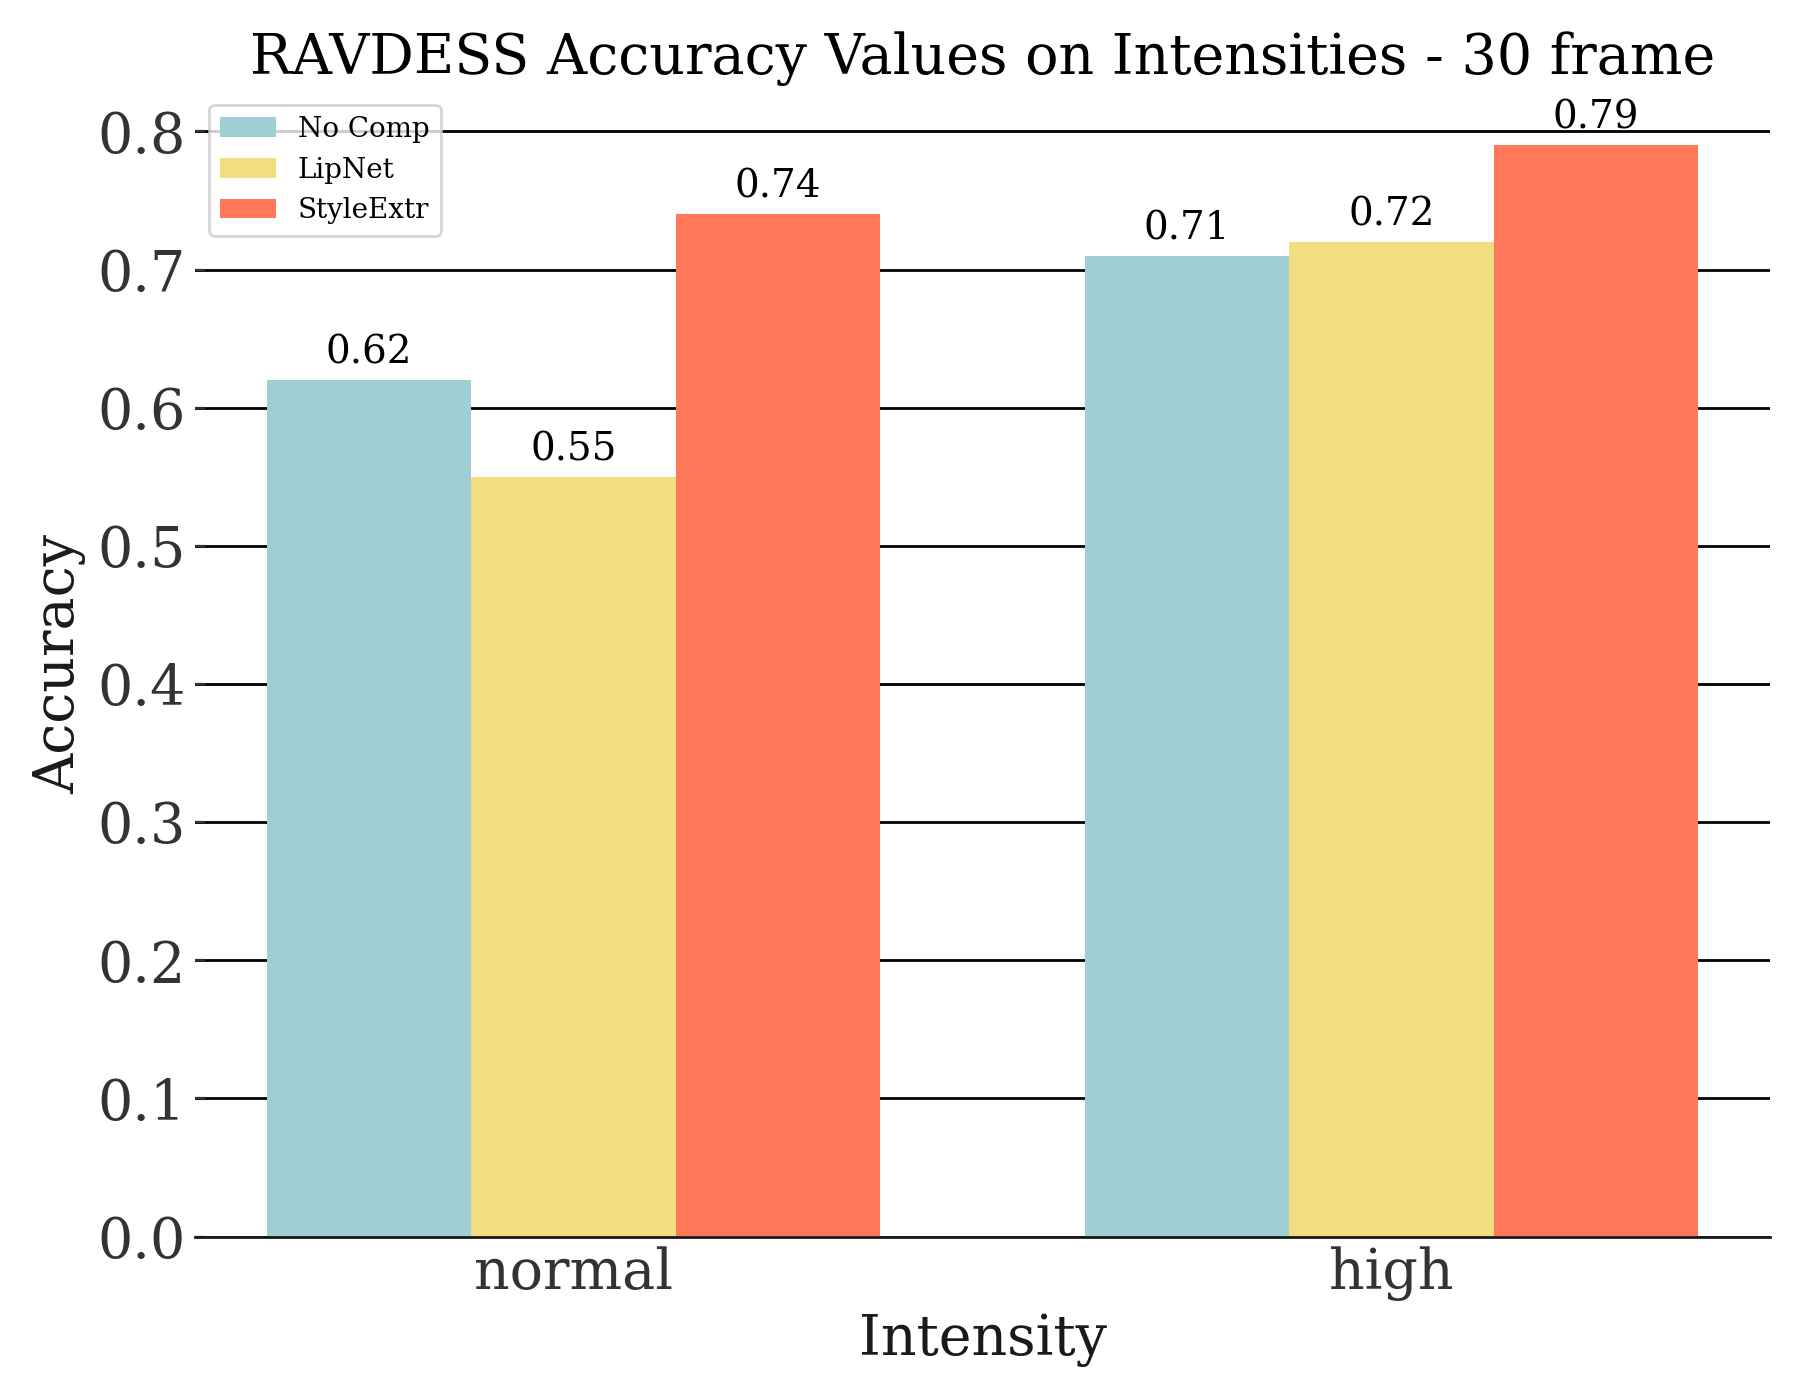
\includegraphics[width=\textwidth]{res/rd-intensities-30.png}
    \end{subfigure}
    \begin{subfigure}[b]{0.45\textwidth}
      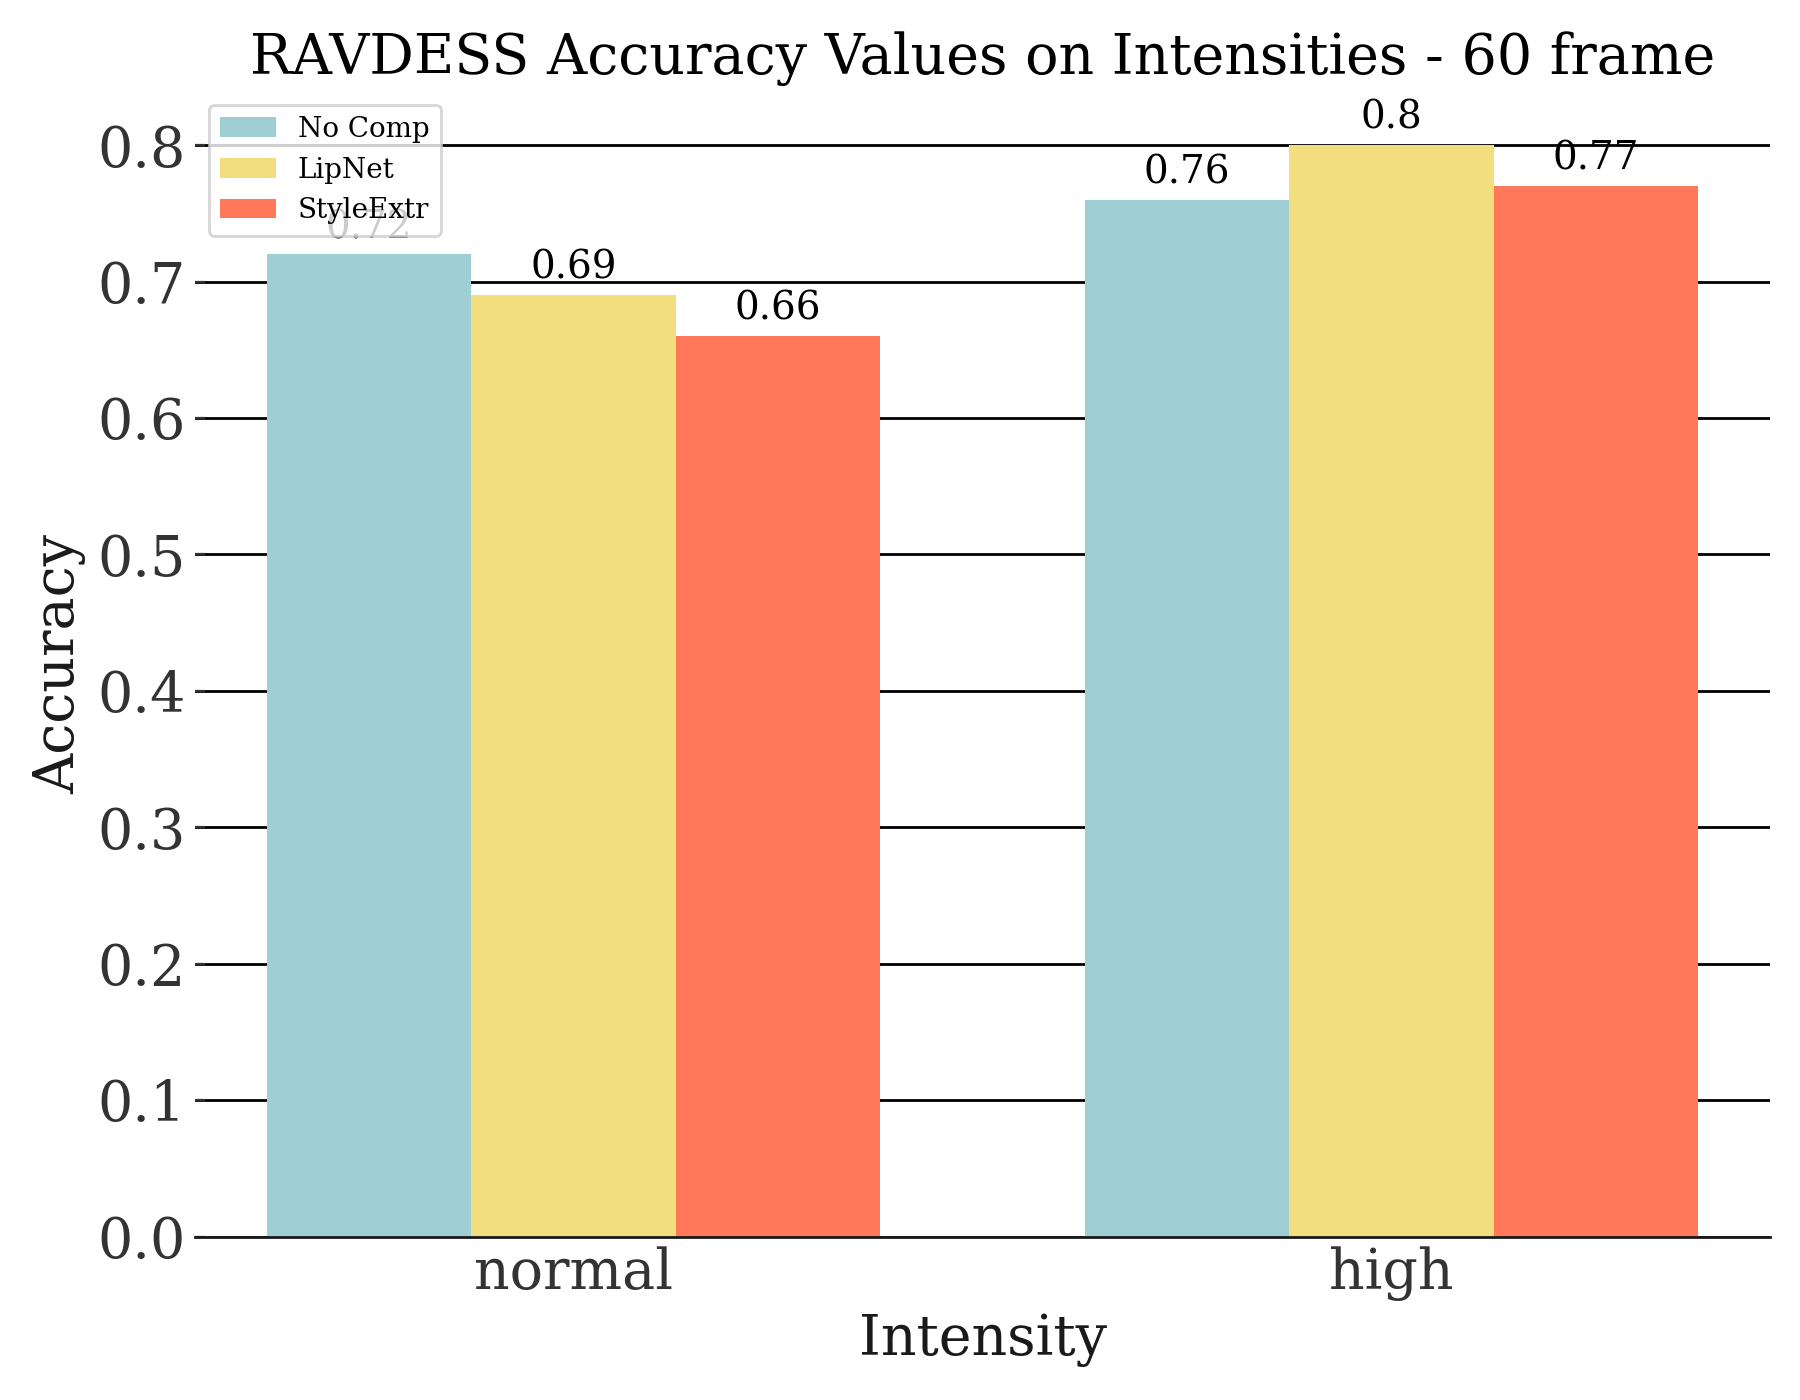
\includegraphics[width=\textwidth]{res/rd-intensities-60.png}
    \end{subfigure}
    \begin{subfigure}[b]{0.45\textwidth}
      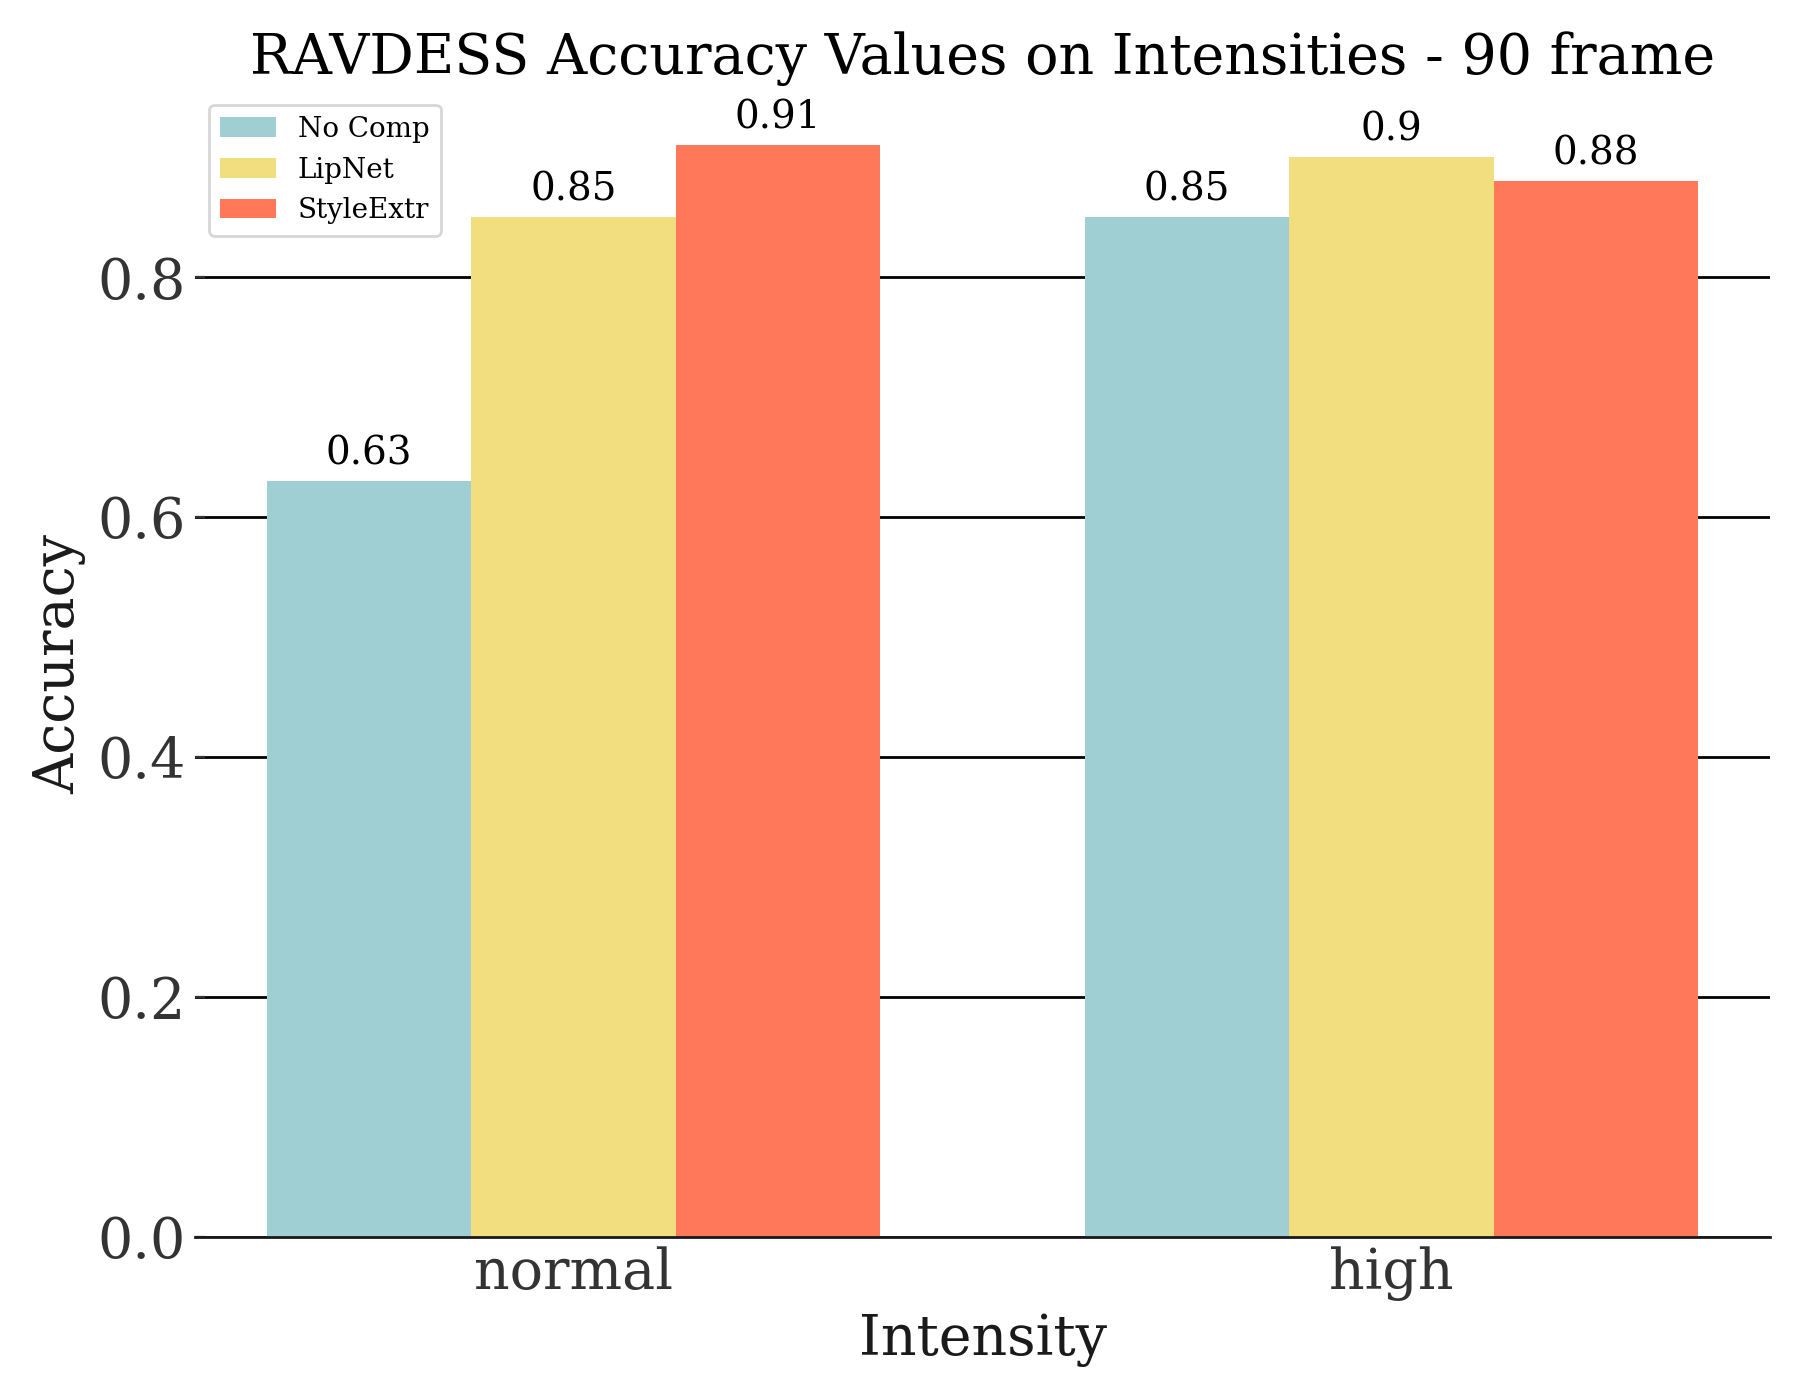
\includegraphics[width=\textwidth]{res/rd-intensities-90.png}
    \end{subfigure}
    \caption{Performance of the models based on the intensity value on the RAVDESS validation set. Neutral videos only had a recordings of \texttt{normal} intensity.}
    \label{fig:rd_intensity}
\end{figure}

\begin{figure}
    \centering
    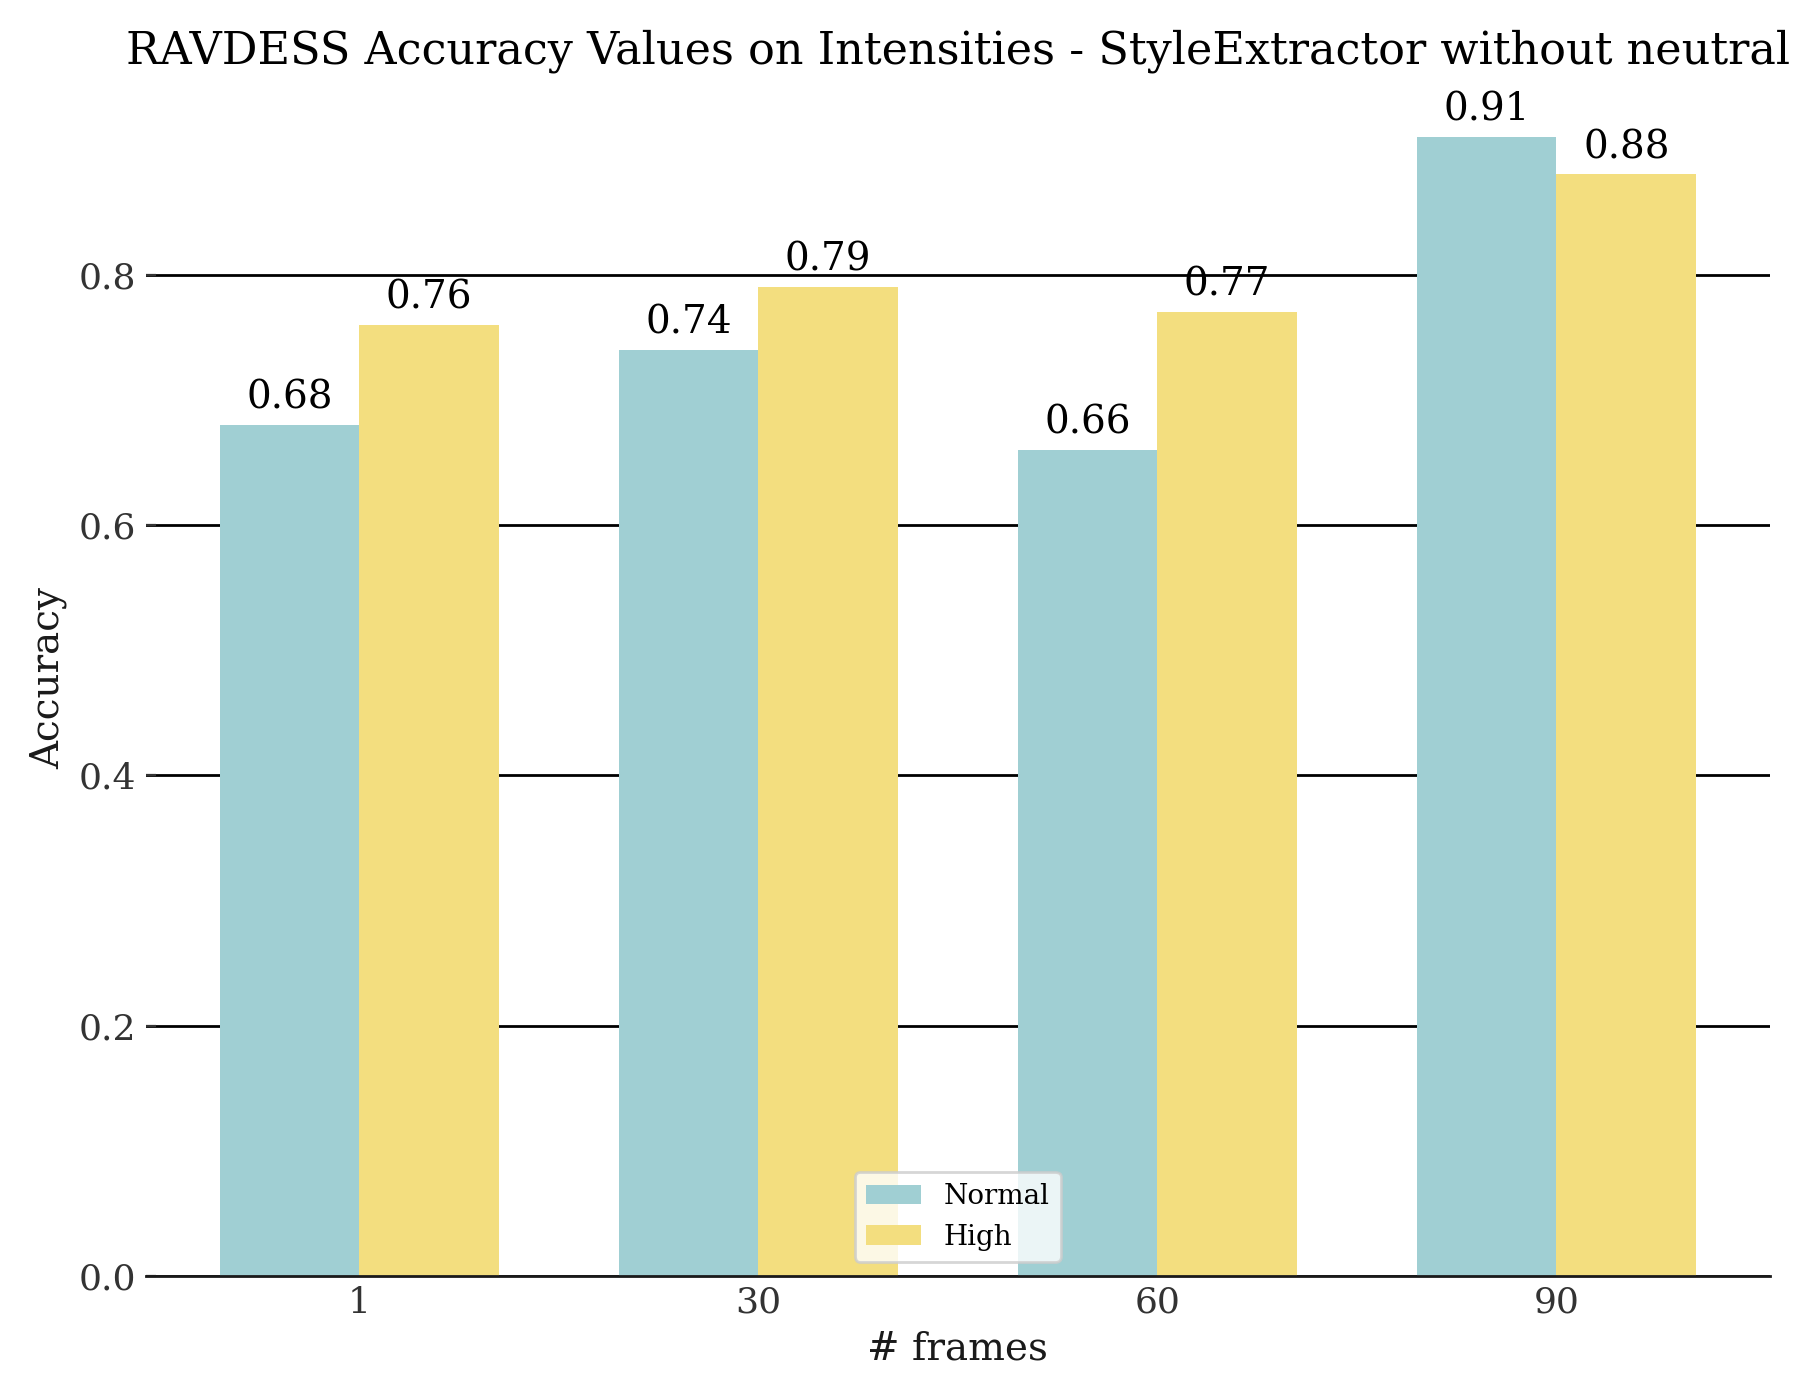
\includegraphics[width=0.8\textwidth]{res/rd-intensities-busso-no-normal.png}
    \caption{The difference in validation accuracy on the FER-SE model without \texttt{neutral} videos. The \texttt{neutral} videos underfit on the FER-SE model, and since they all are inherently set to a \texttt{normal} intensity the previous results in figure \ref{fig:rd_intensity} are skewed.}
    \label{fig:busso_no_normal}
\end{figure}

\subsubsection{Cross Dataset Validation}
\label{sec:cross_dataset}

\begin{figure}
    \centering
    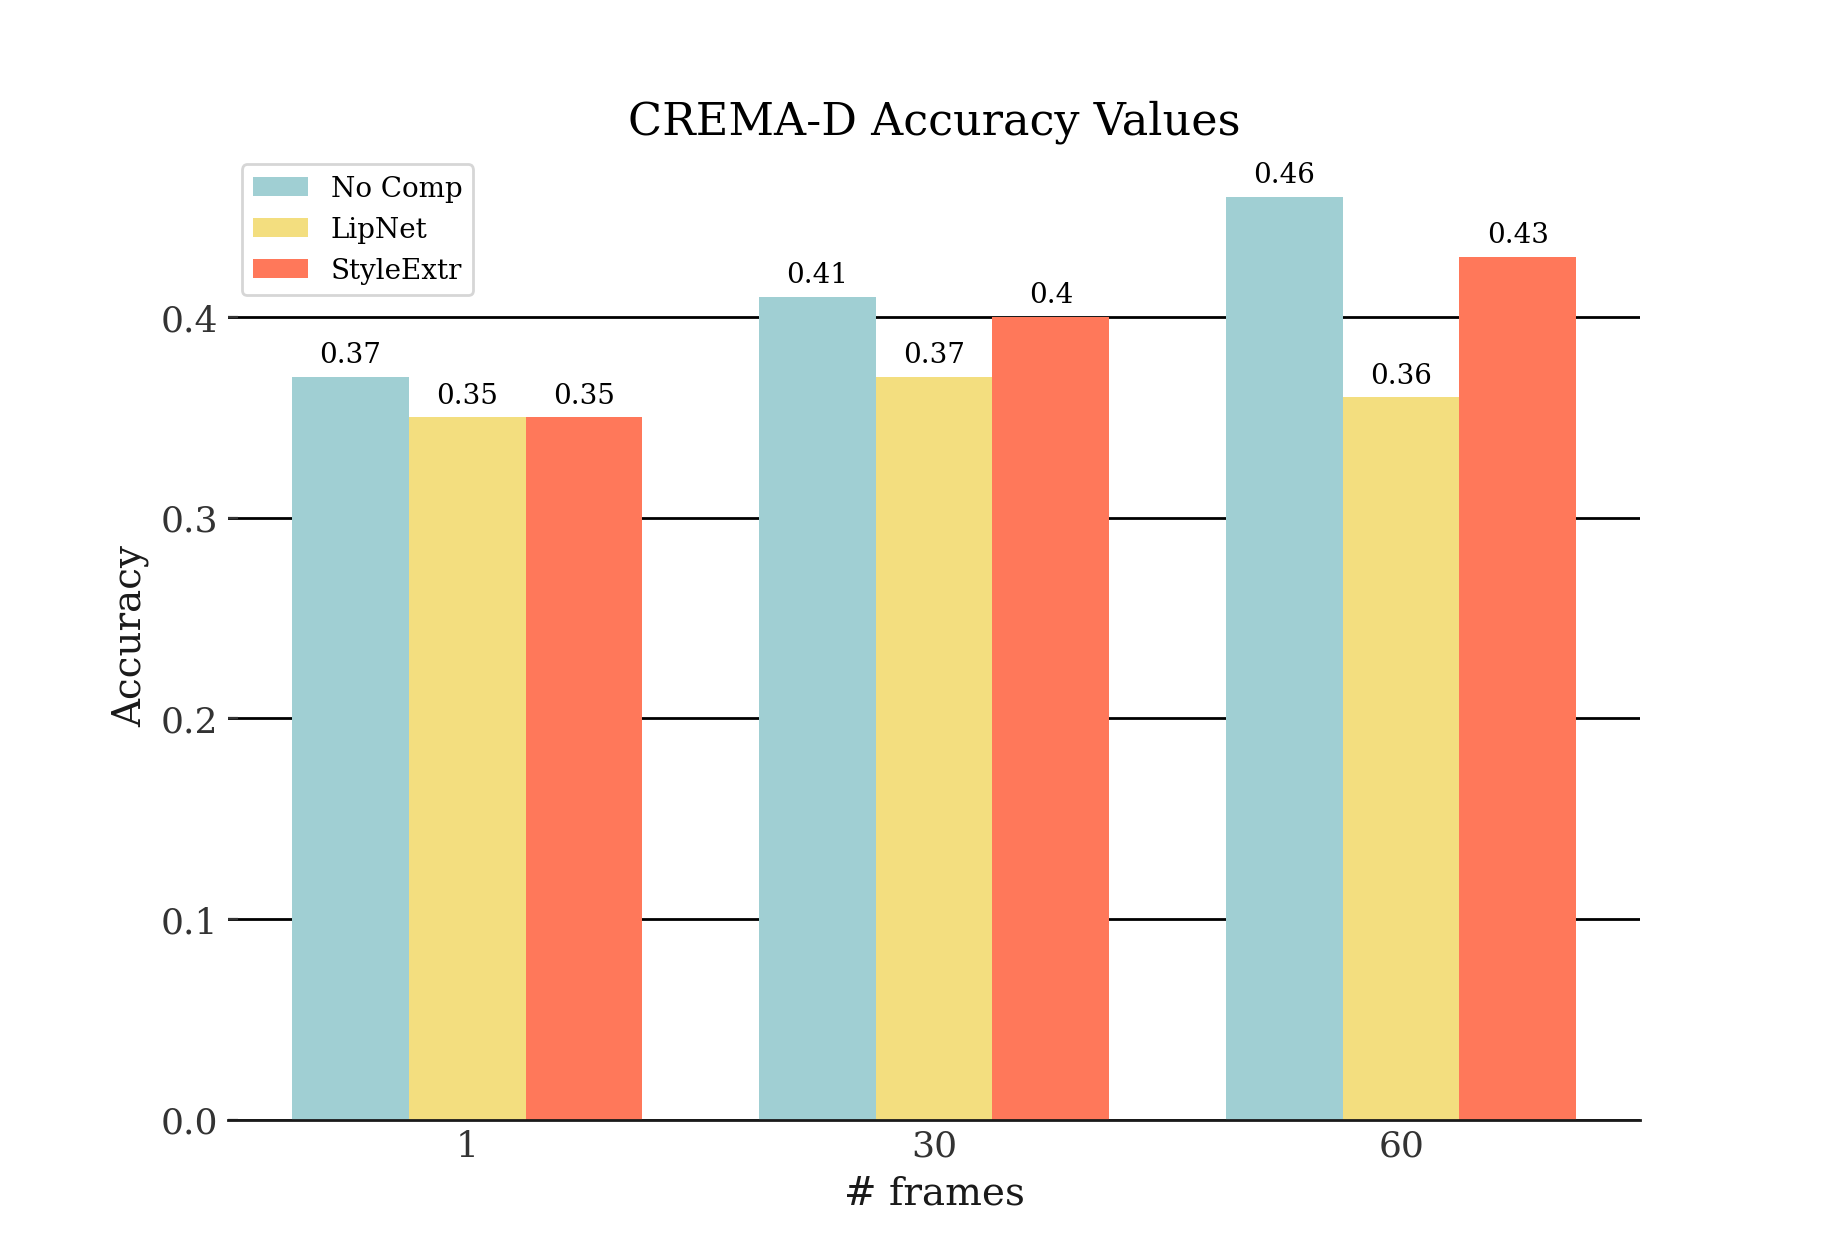
\includegraphics[width=0.8\textwidth]{res/CremaValidation.png}
    \caption{Validation results of the our models on the CREMA-D corpus. A result for 90 frames was not possible since most videos in the CREMA-D database are not long enough.}
    \label{fig:crema_val_lipnet}
\end{figure}

All our models on the FER section were trained on RAVDESS. An interesting question is if and how well the models generalize to other datasets, in this case CREMA-D. We ran validation on all our models using the CREMA-D corpus and compared the results \ref{fig:crema_val_lipnet}. We could not run the models trained on 90 frames since the videos in the CREMA-D database do not have enough frames.

\paragraph{General Results}
Looking at the performance of the FER model, we see a continued trend for the importance of the existence and magnitude of the temporal compensator. An increase in frame-window size from one to 60 improved the results by 24\%, or nine percentage points. An better performance can also be observed compared to the FER-LN model. The FER-TC model consistently performs better than its FER-LN counterpart, up to 28\%, or ten percentage points. The FER-LN model itself did not benefit from the temporal dimension. Its performance was between 35\% and 37\% throughout the different frame-window sizes. The FER-SE model however also continued the trend of improvement with more temporal information. It also performs worse than the FER-TC model, within a margin of one to three percentage points. 

The performance of the FER-SE model compared to the FER-LN model on domain shifts point to issues in using and training lexical compensators. A more robust and specialized lexical compensator produces better results than an off-the-shelve, tangentially related model. However, even the FER-SE model performed worse than the FER-TC model. A combination of two models will produce compound errors, which can be managed by training on more diverse datasets.

\paragraph{Intensities}
We also analysed the performance on CREMA-D based on the labelled intensity for each video (Figure \ref{fig:crema_intesities}). An interesting pattern emerges. At lower frames the FER-SE performs significantly better on \texttt{low} and \texttt{medium} intensity recordings compared to the other models. \texttt{High} and \texttt{low} intensity recordings are estimated more accurately than those of \texttt{medium} intensity. When increasing the frame-window size, the FER-TC model improves significantly. The models with compensators do not gain as much accuracy, especially the FER-LN model which stays similar in accuracy throughout all frame-window sizes. These results are different from the ones in section \ref{sec:model_results}. On the RAVDESS dataset we saw a definitive increase in accuracy on higher intensity recordings. The RAVDESS corpus did not provide \texttt{low} intensity videos. Its \texttt{normal} intensity is comparable to the \texttt{medium} intensity of CREMA-D.


\begin{figure}[!htb]
    \centering
    \begin{subfigure}[b]{0.45\textwidth}
      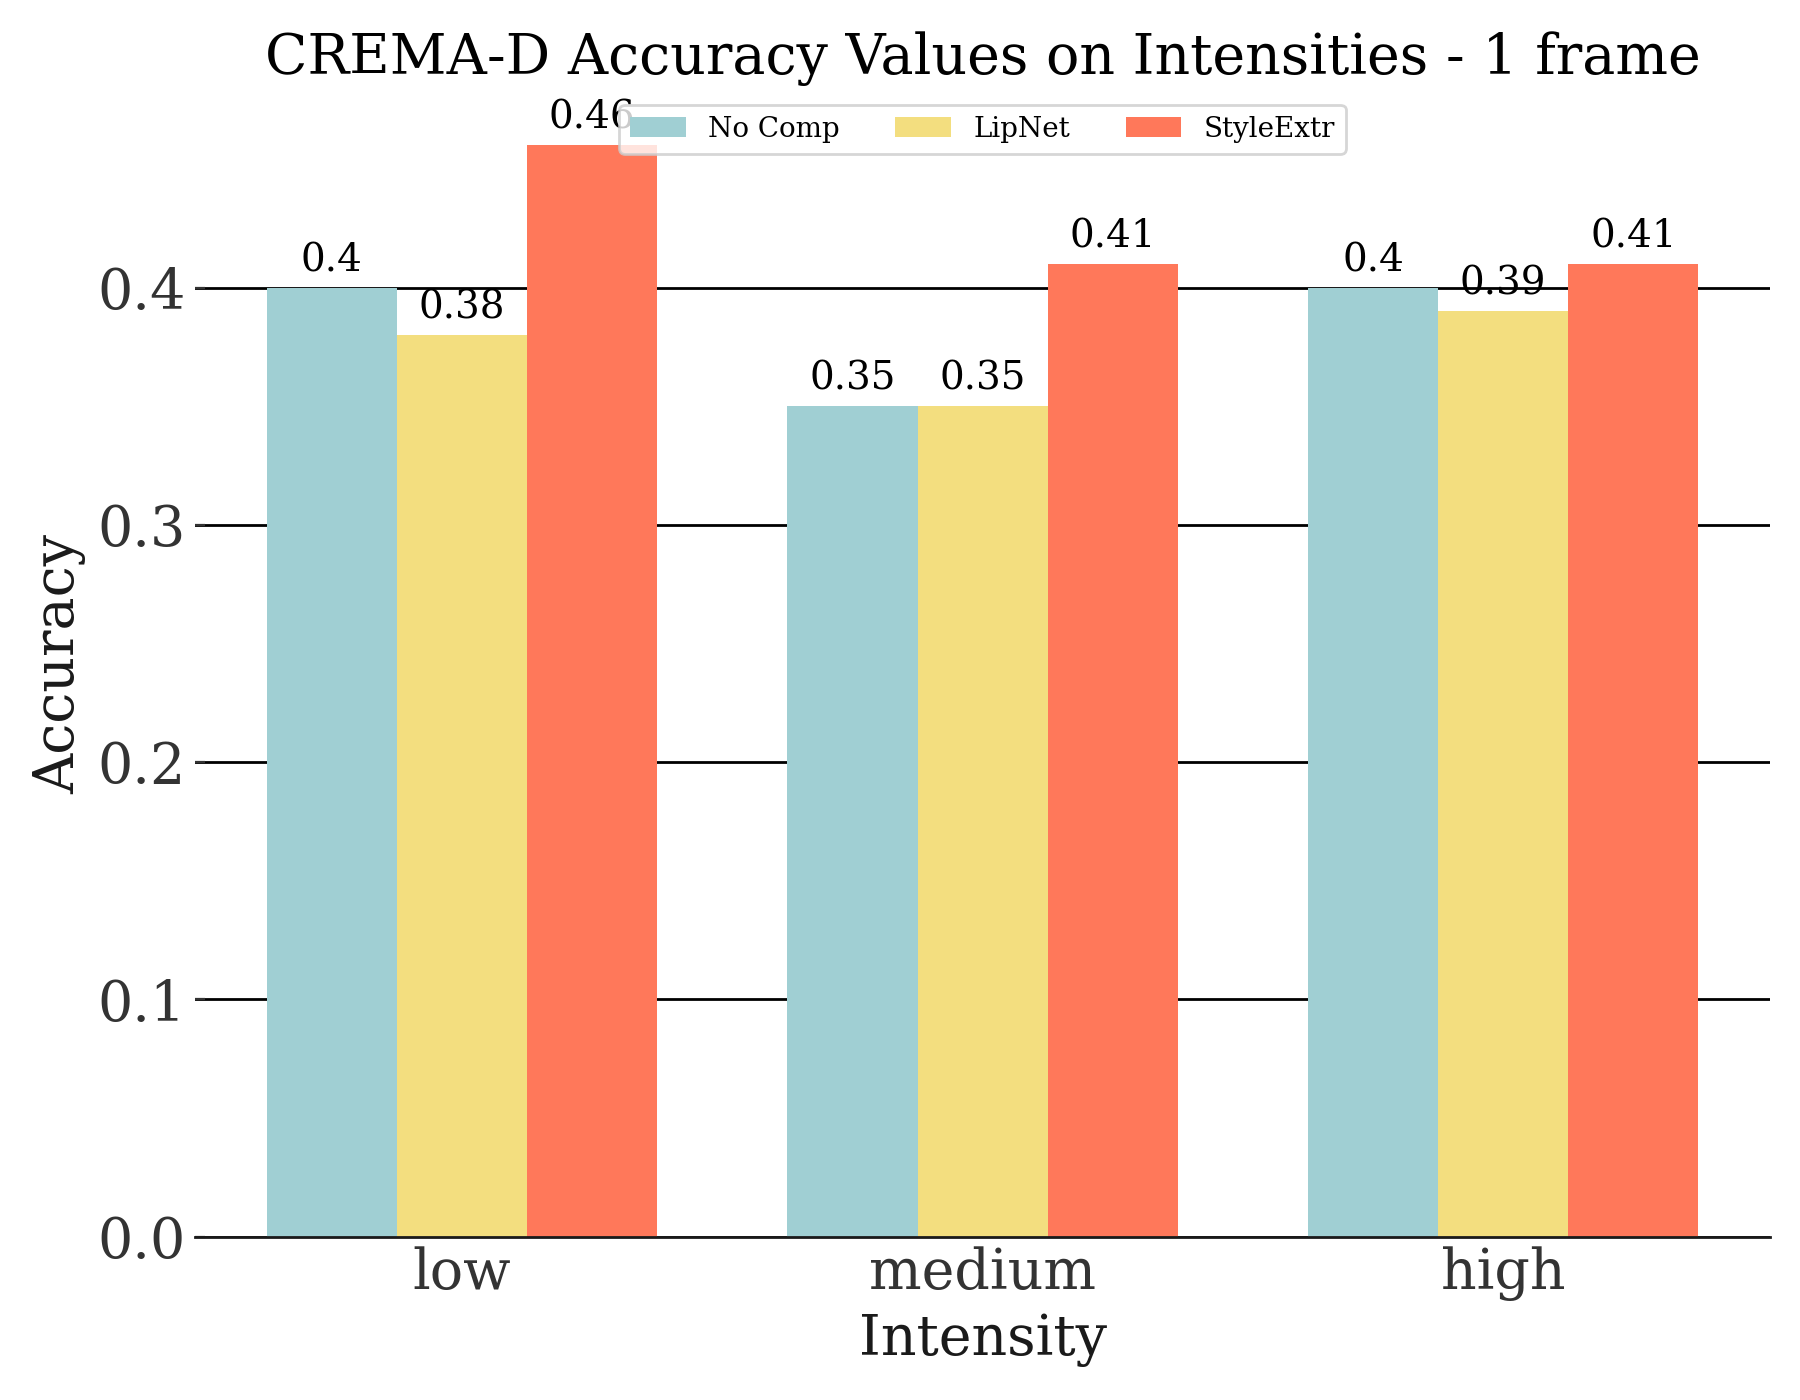
\includegraphics[width=\textwidth]{res/crema-intensities-1.png}
    \end{subfigure}
    \begin{subfigure}[b]{0.45\textwidth}
      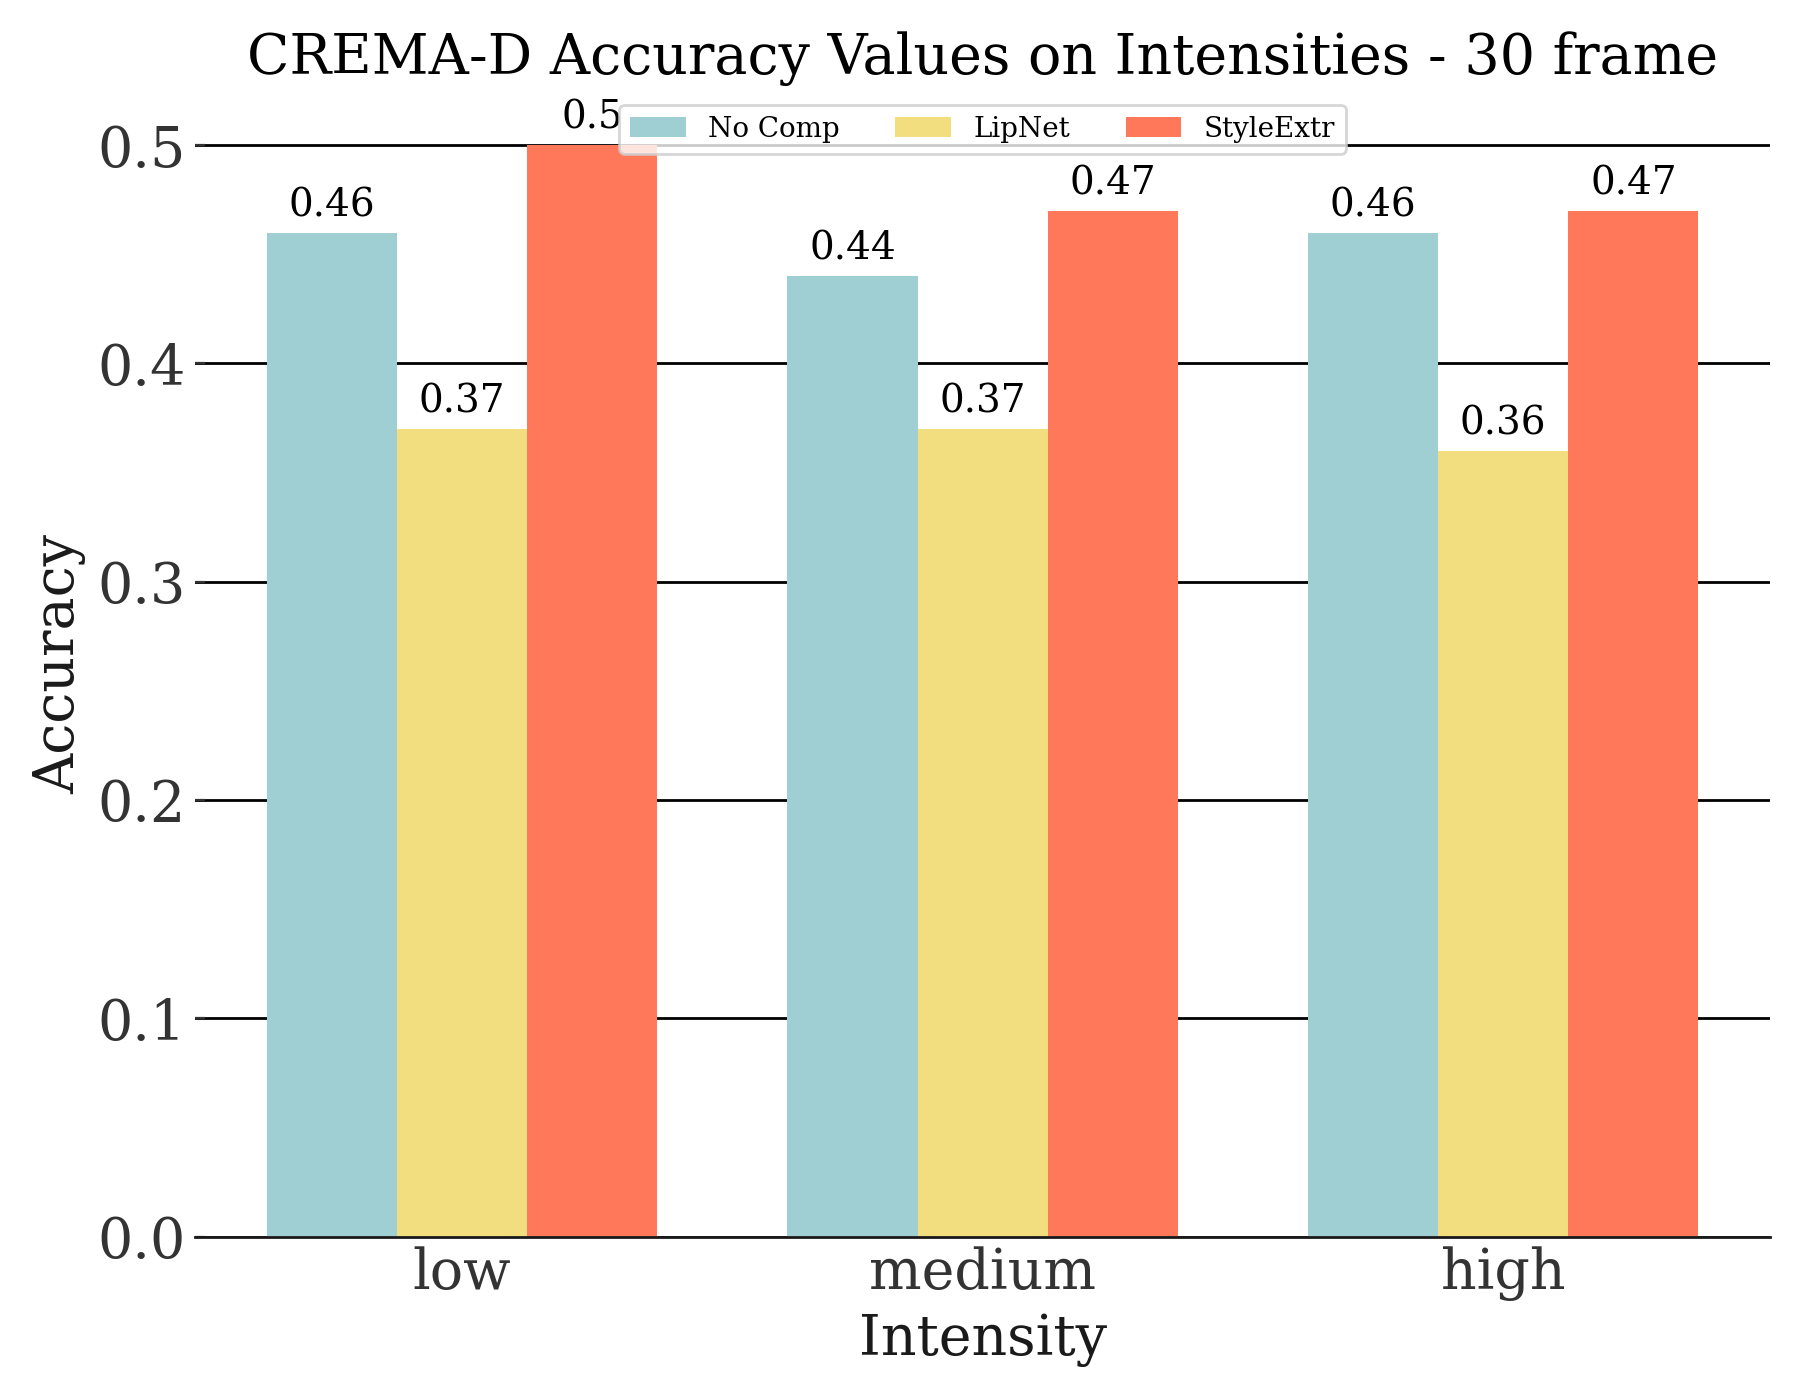
\includegraphics[width=\textwidth]{res/crema-intensities-30.png}
    \end{subfigure}
    \begin{subfigure}[b]{0.45\textwidth}
      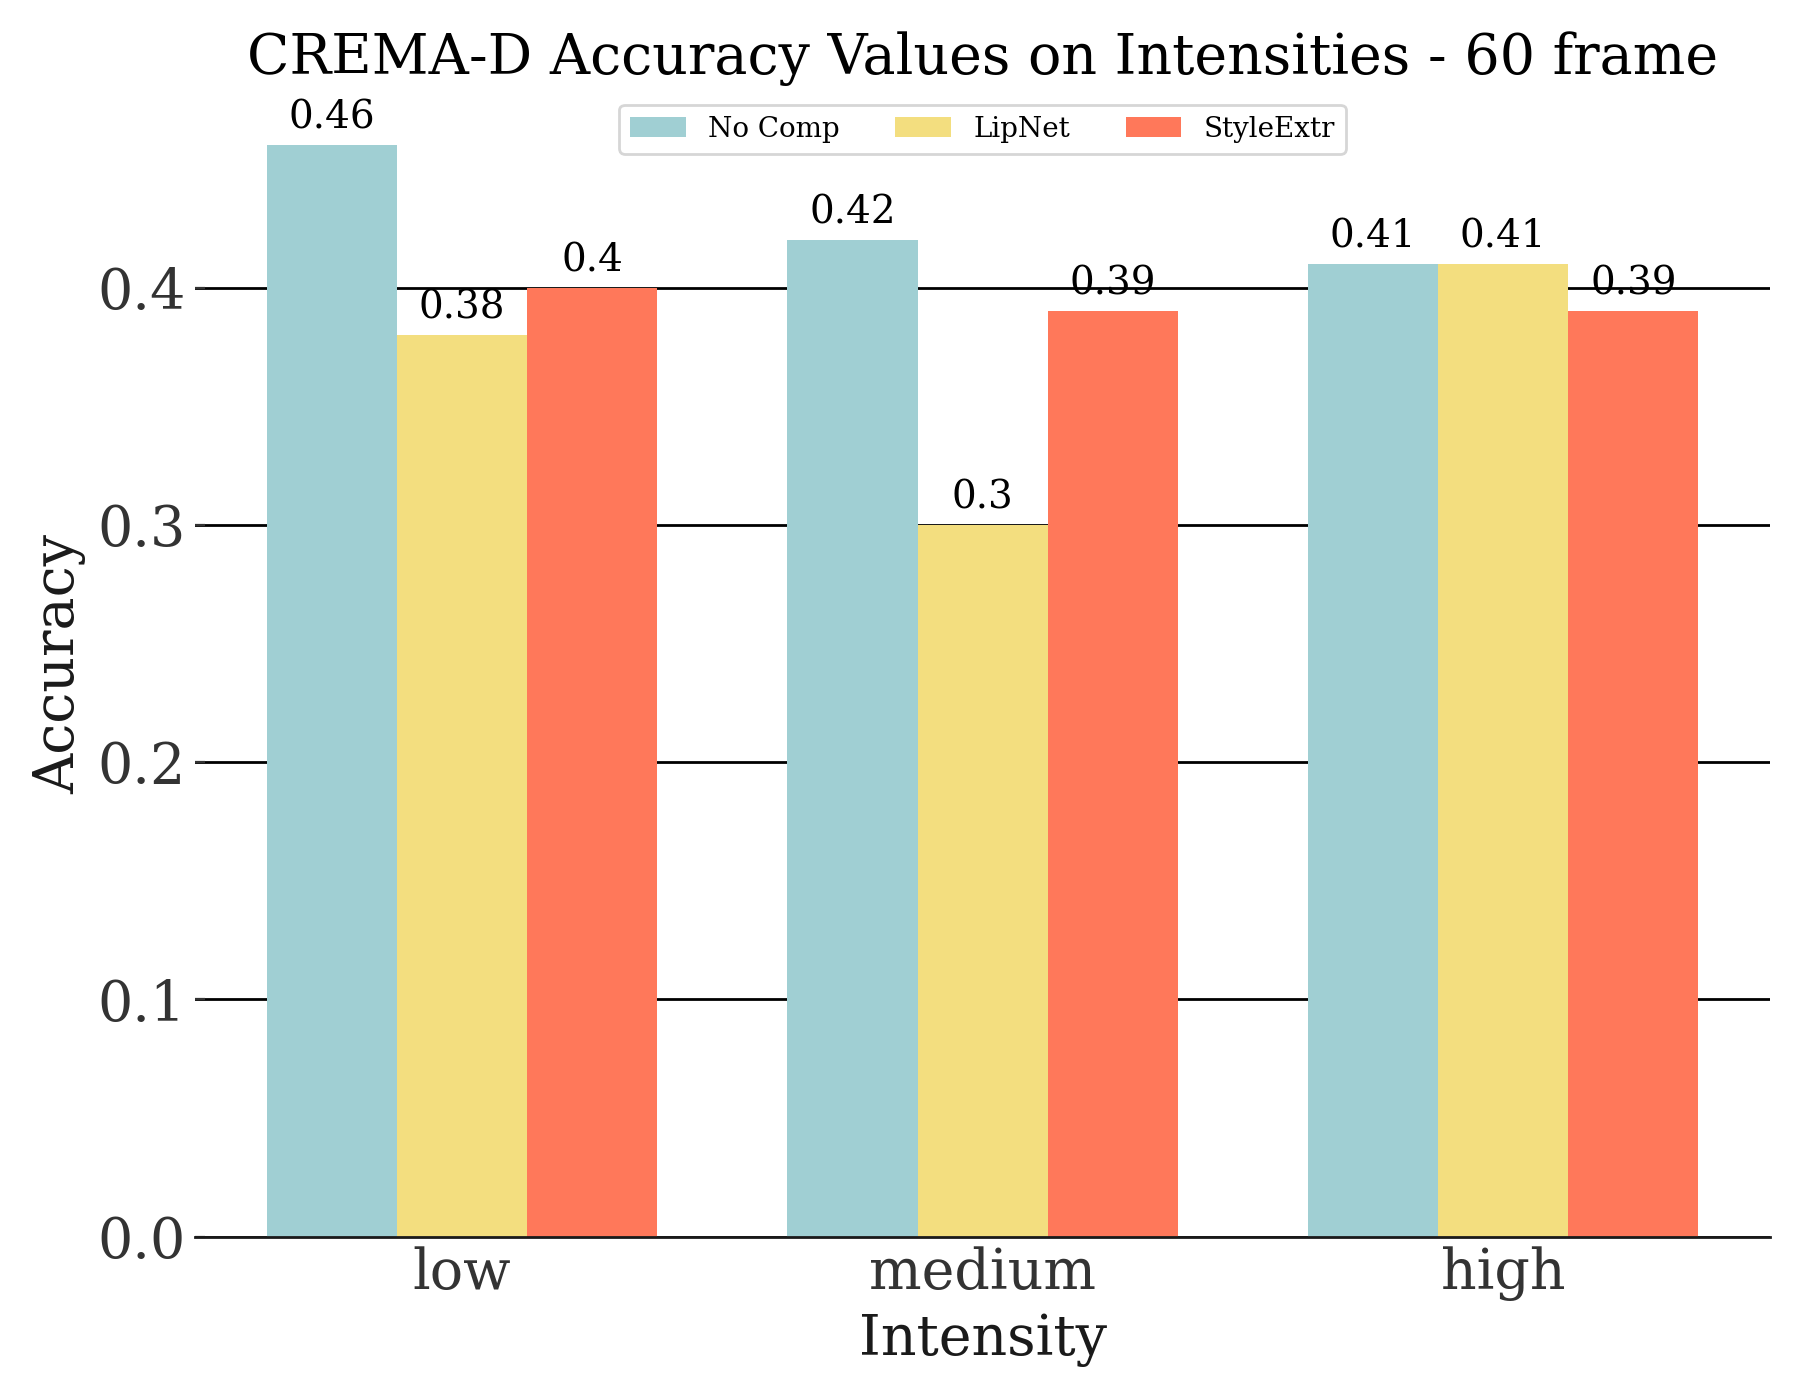
\includegraphics[width=\textwidth]{res/crema-intensities-60.png}
    \end{subfigure}
    \caption{Validation accuracies of our models on the CREMA-D corpus depending on the intensity by which the emotions were expressed.}
    \label{fig:crema_intesities}
\end{figure}

\subsubsection{Phonetic (In-)Dependence}
In section \ref{sec:human} we already saw that the phonetic performance of existing FER models was low and varied between phonemes. After training our single-frame models, we run the same analysis again to determine the improvements in phonetic performance and to figure out if and how the lexical compensators impact the results.

We ran the same test as we did in section \ref{sec:human} on the validation set of RAVDESS (Actors 4 and 5) with the models we trained with a frame-window size of one. All three models perform very similarly, struggling and having higher accuracy on the same phonemes. The lexical compensators thus do not increase performance or robustness on a phonetic level.

We conclude that the lexical compensators, as we implemented them, do not replicate the results of human benchmarking, where our annotators were able to predict the underlying emotions on a similar level of accuracy independent of the phoneme. In the case of the FER-SE model, we implemented the style extractor without the secondary phoneme-prediction like Salman and Busso did \cite{salman2020style}. This secondary prediction, even if it was later unused, might have been beneficial when training the style extractors mesh transformation in guiding it towards phonetic recognition.

\begin{figure}
    \centering
    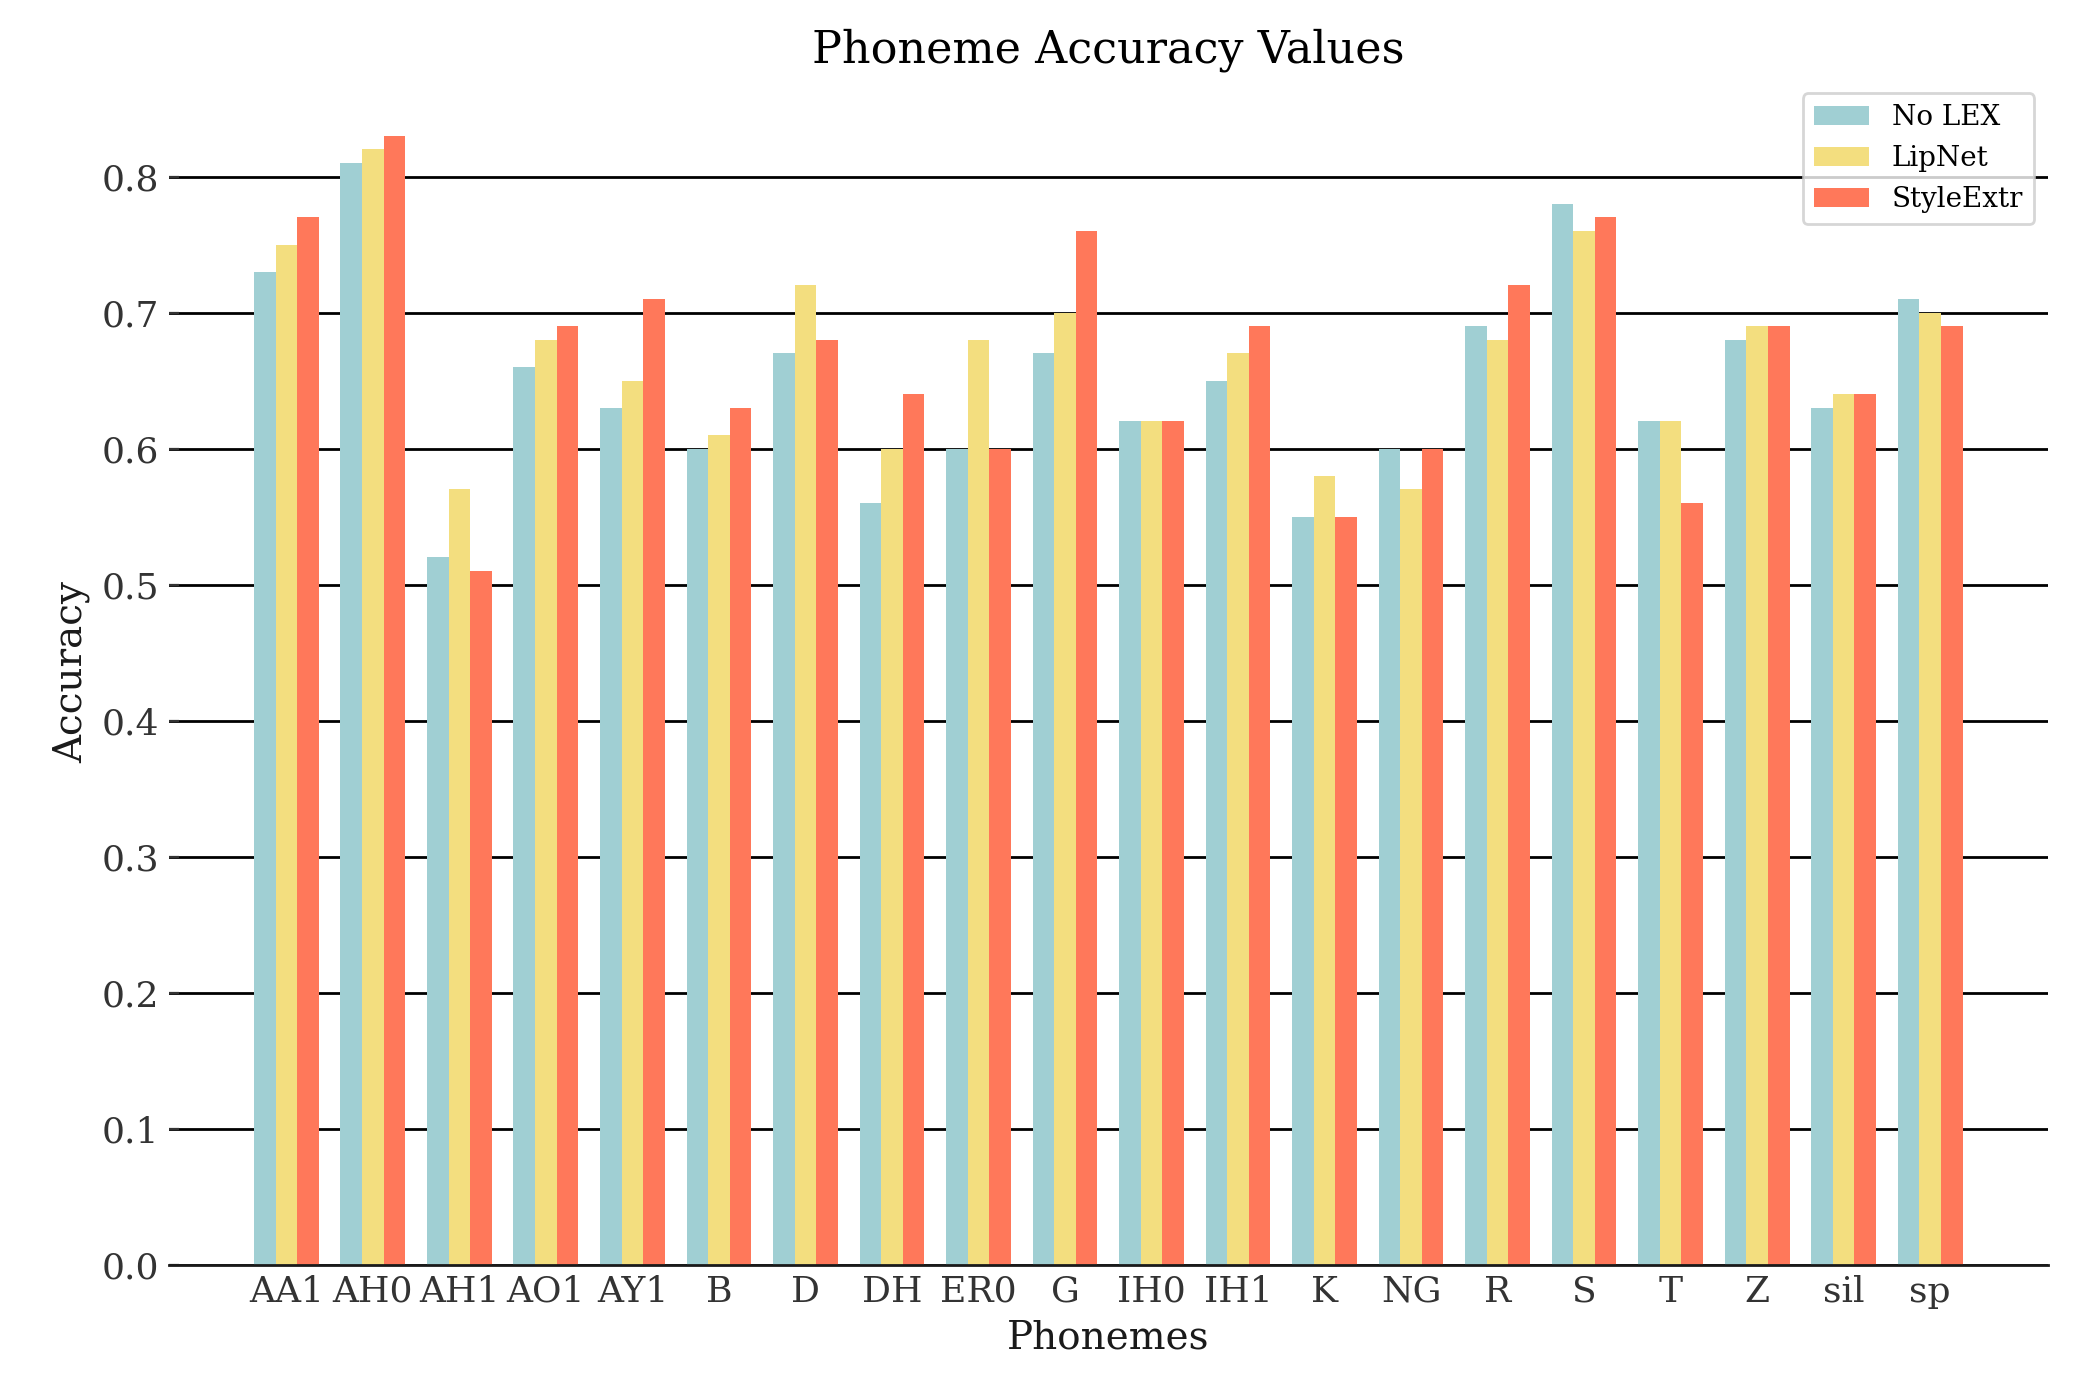
\includegraphics[width=0.8\textwidth]{res/ModelsOnPhones.png}
    \caption{Evaluating the models we trained with a frame-window size of one based on the phoneme spoken in the frame. There is no significant difference on whether a lexical compensator is used or not.}
    \label{fig:modelsonphones}
\end{figure}

\subsubsection{Computational Performance}
\label{sub:computational}
In practical applications, strong and robust performance in accuracy is important in FER models, but certainly not the only metric by which we judge them. Other factors, like application range and computational complexity are also reasons to use one model over another. We have three different models that are very similar in validation accuracy during training, yet differ when it comes to complexity. The temporalized FER model without any lexical compensator is the easiest model to use. It only requires a facial crop of the image, and has no second input which needs to be preprocessed and predicted during model usage. This also makes it the most computationally performant model. The model using LipNet as its compensator also has easy preprocessing steps, needing an additional crop of the orofacial area. The pruned part of LipNet that we use has 327648 parameters, and does make up a large part of the total network size. While the model with the style extractor has a similar size with 361468 parameters, it also needs to run a FaceMesh preprocessing step for its input.

All three models are followed up by the fusion/transfer layers, which has a size of 1189511 parameters.
% \begin{figure}
%     \centering
%     \begin{subfigure}[b]{0.45\textwidth}
%       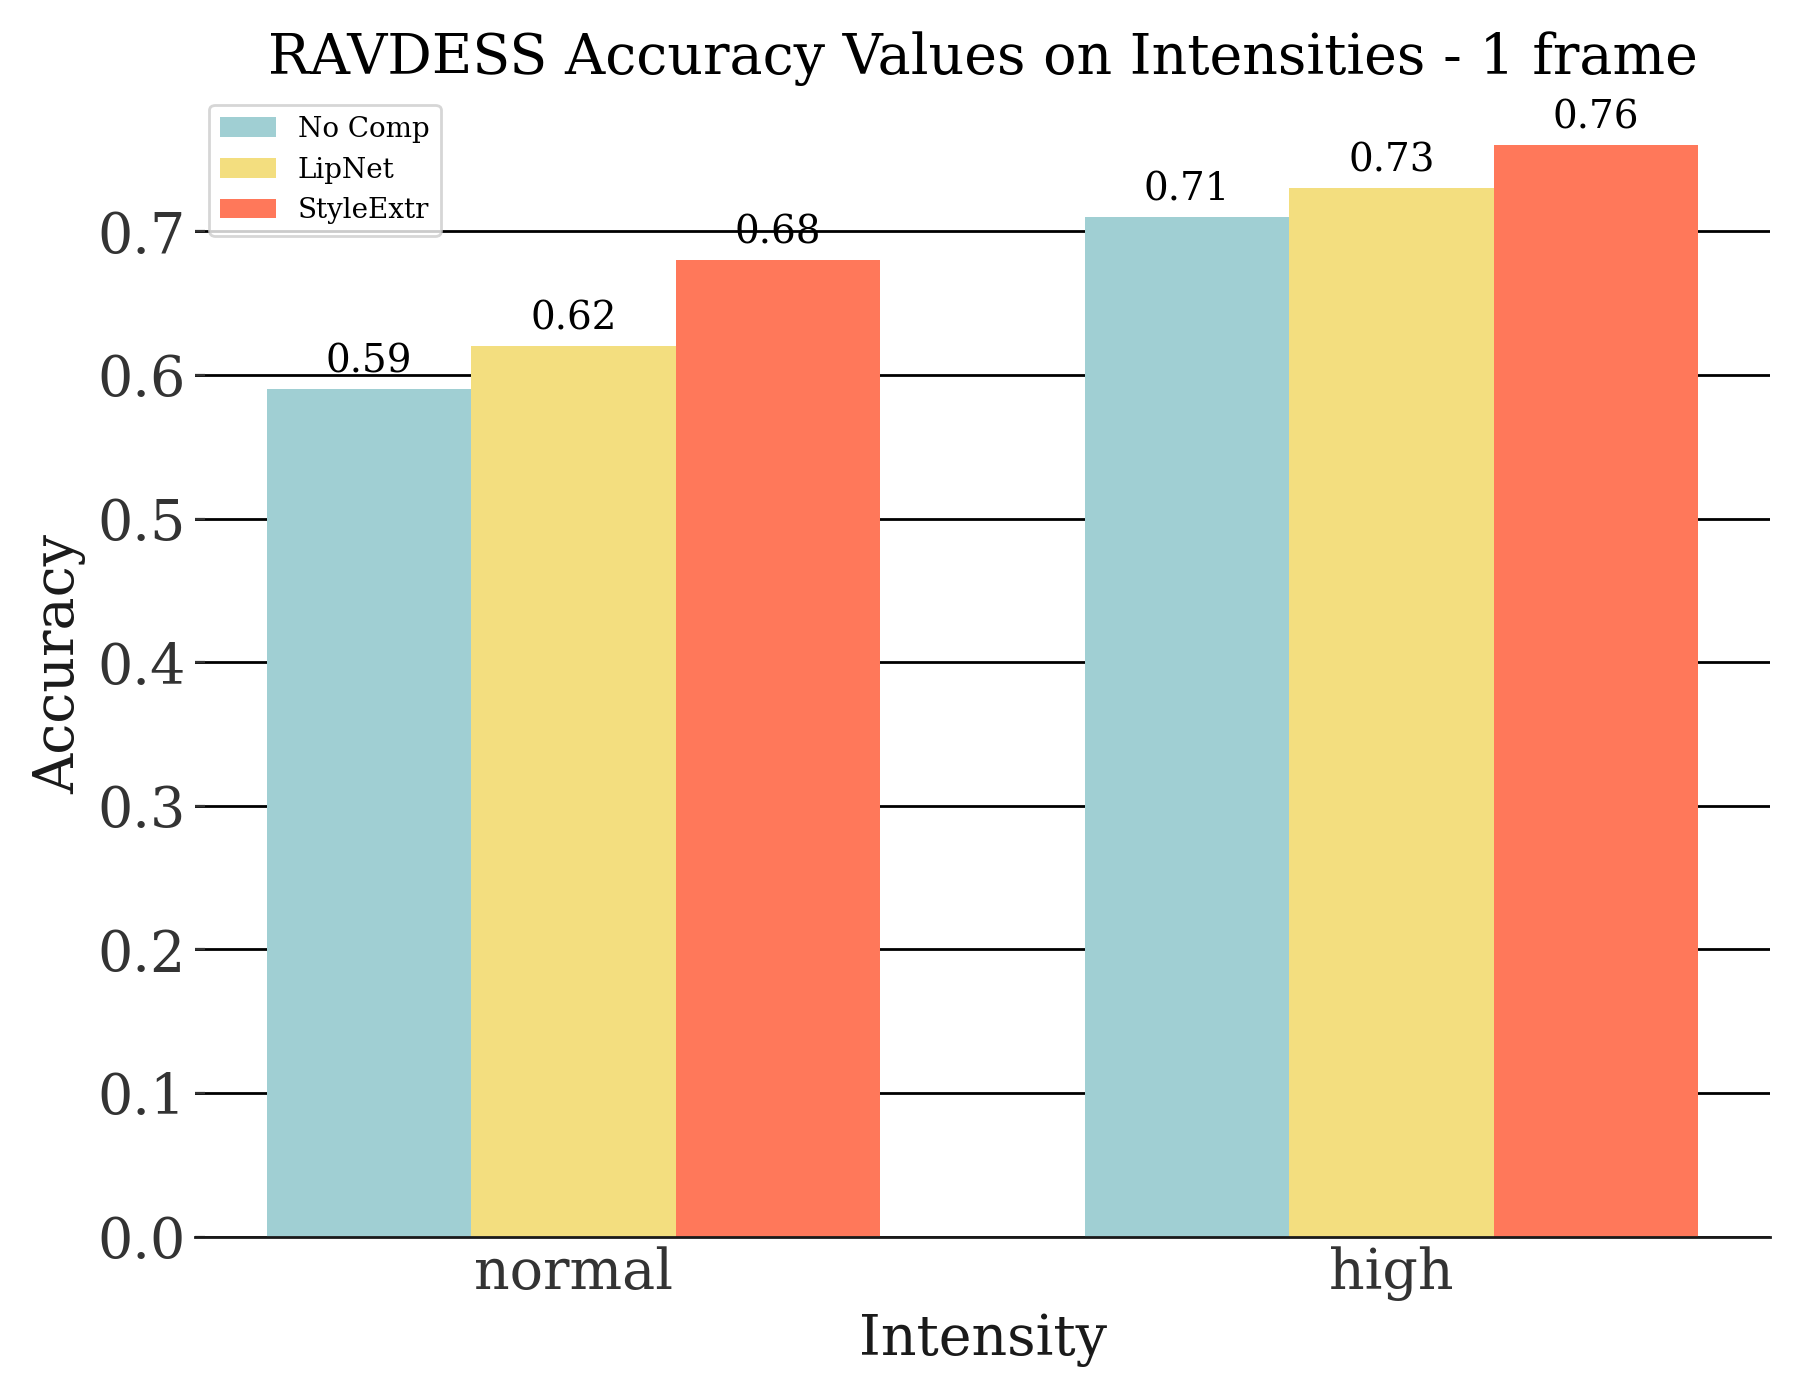
\includegraphics[width=\textwidth]{res/rd-intensities-1.png}
%     \end{subfigure}
%     \begin{subfigure}[b]{0.45\textwidth}
%       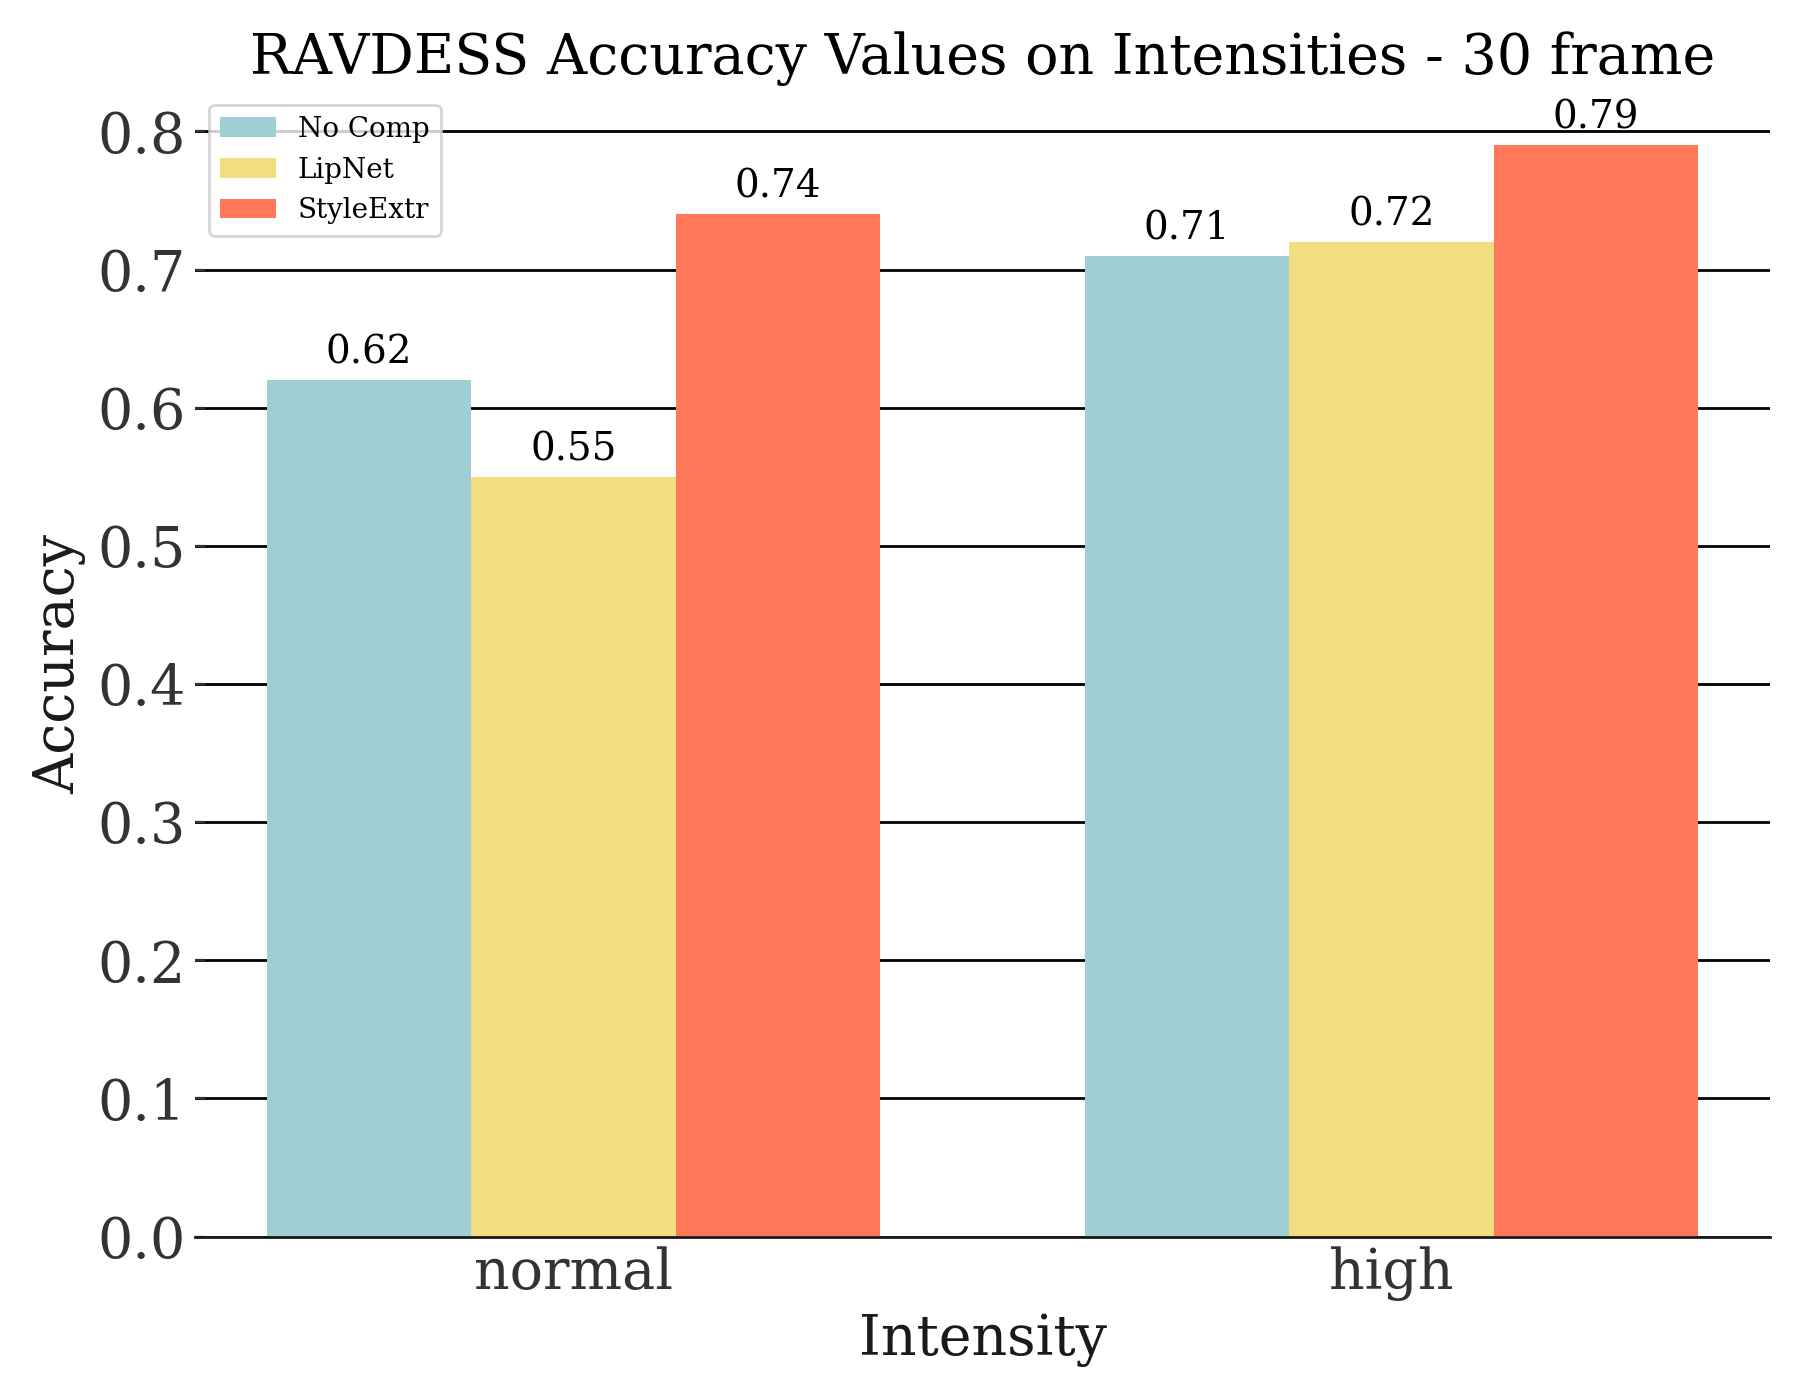
\includegraphics[width=\textwidth]{res/rd-intensities-30.png}
%     \end{subfigure}
%     \begin{subfigure}[b]{0.45\textwidth}
%       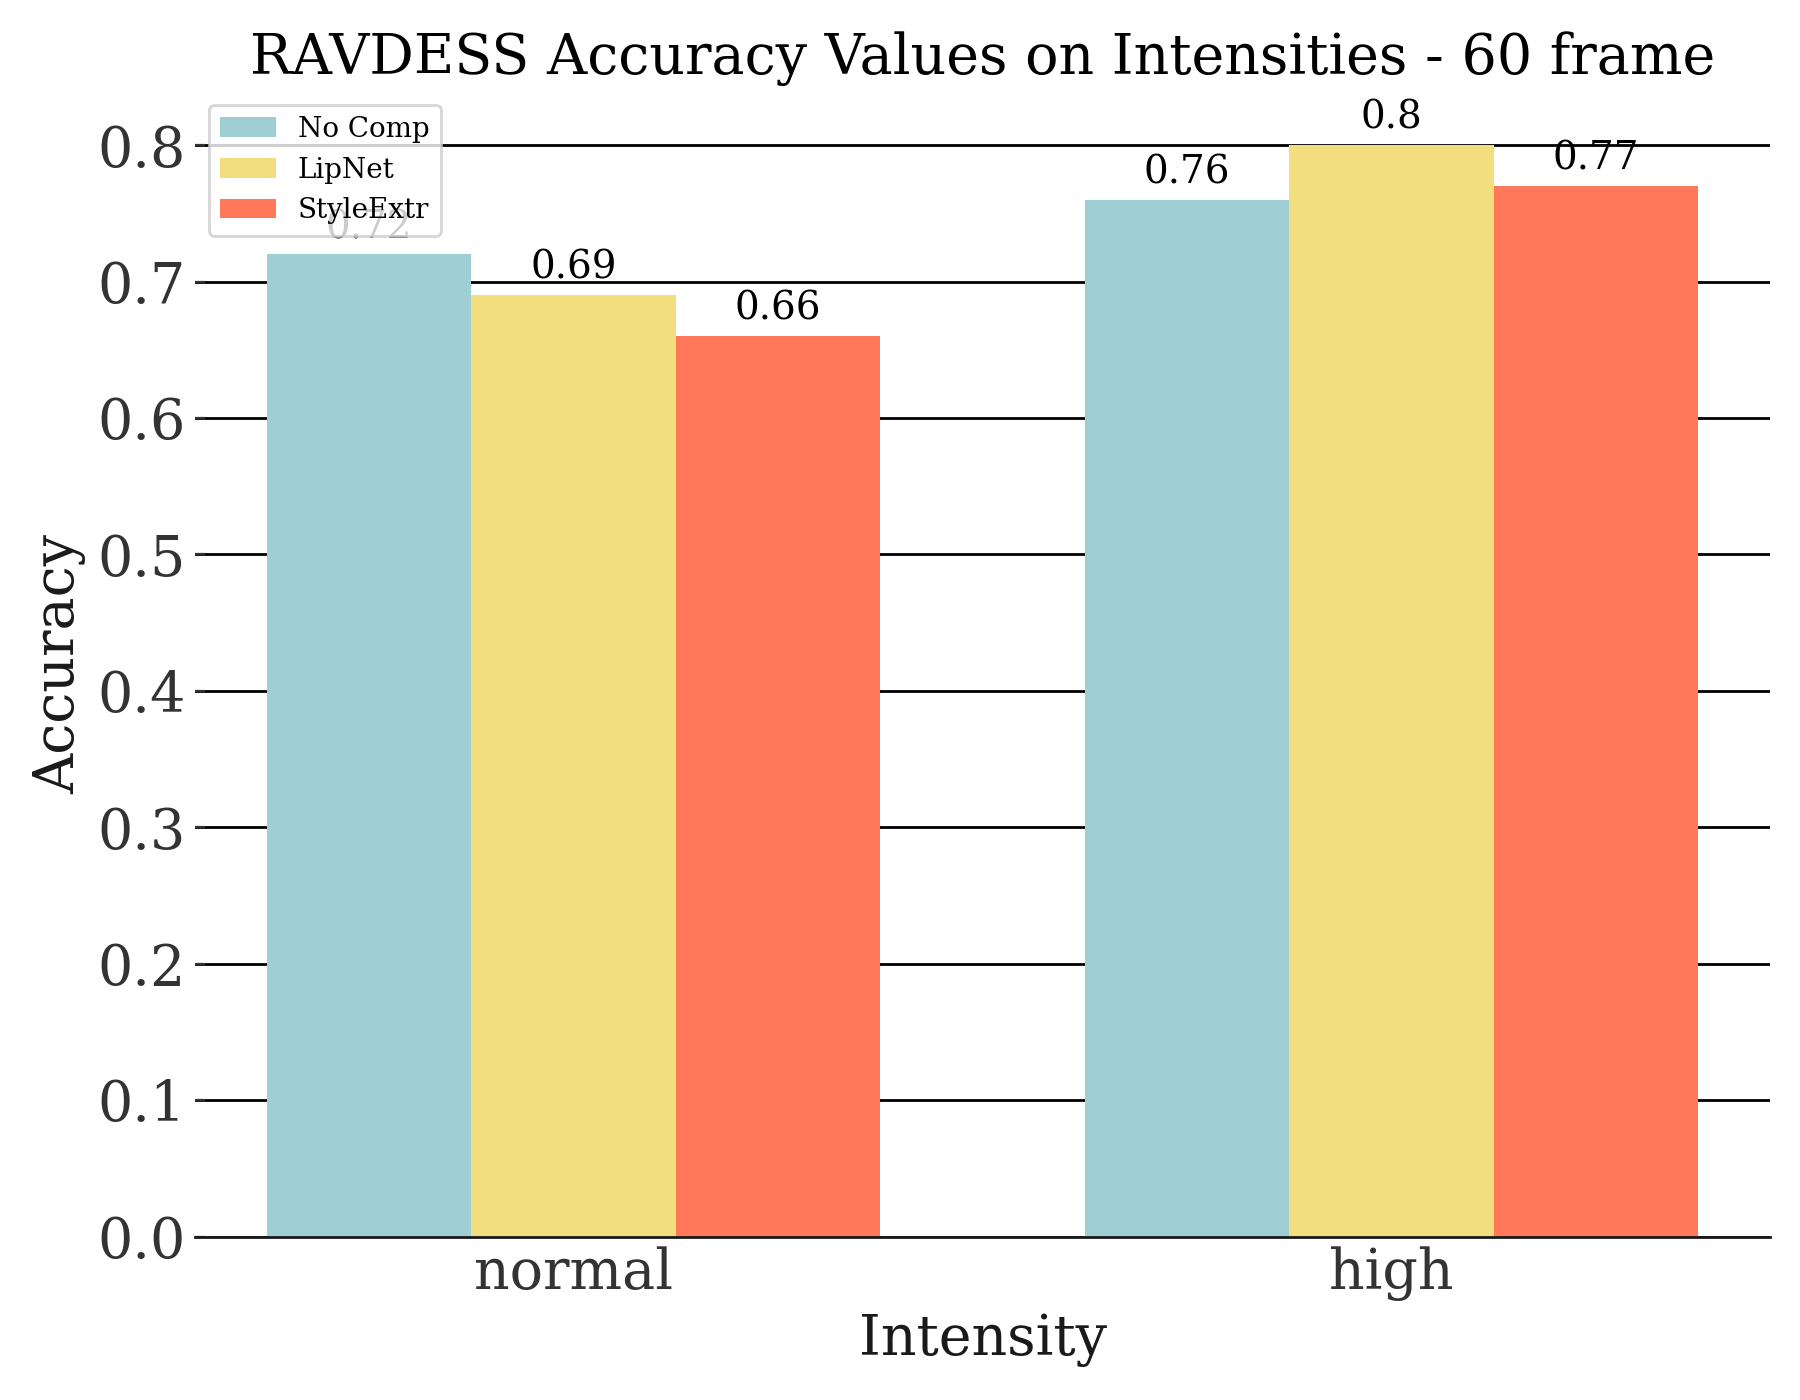
\includegraphics[width=\textwidth]{res/rd-intensities-60.png}
%     \end{subfigure}
%     \begin{subfigure}[b]{0.45\textwidth}
%       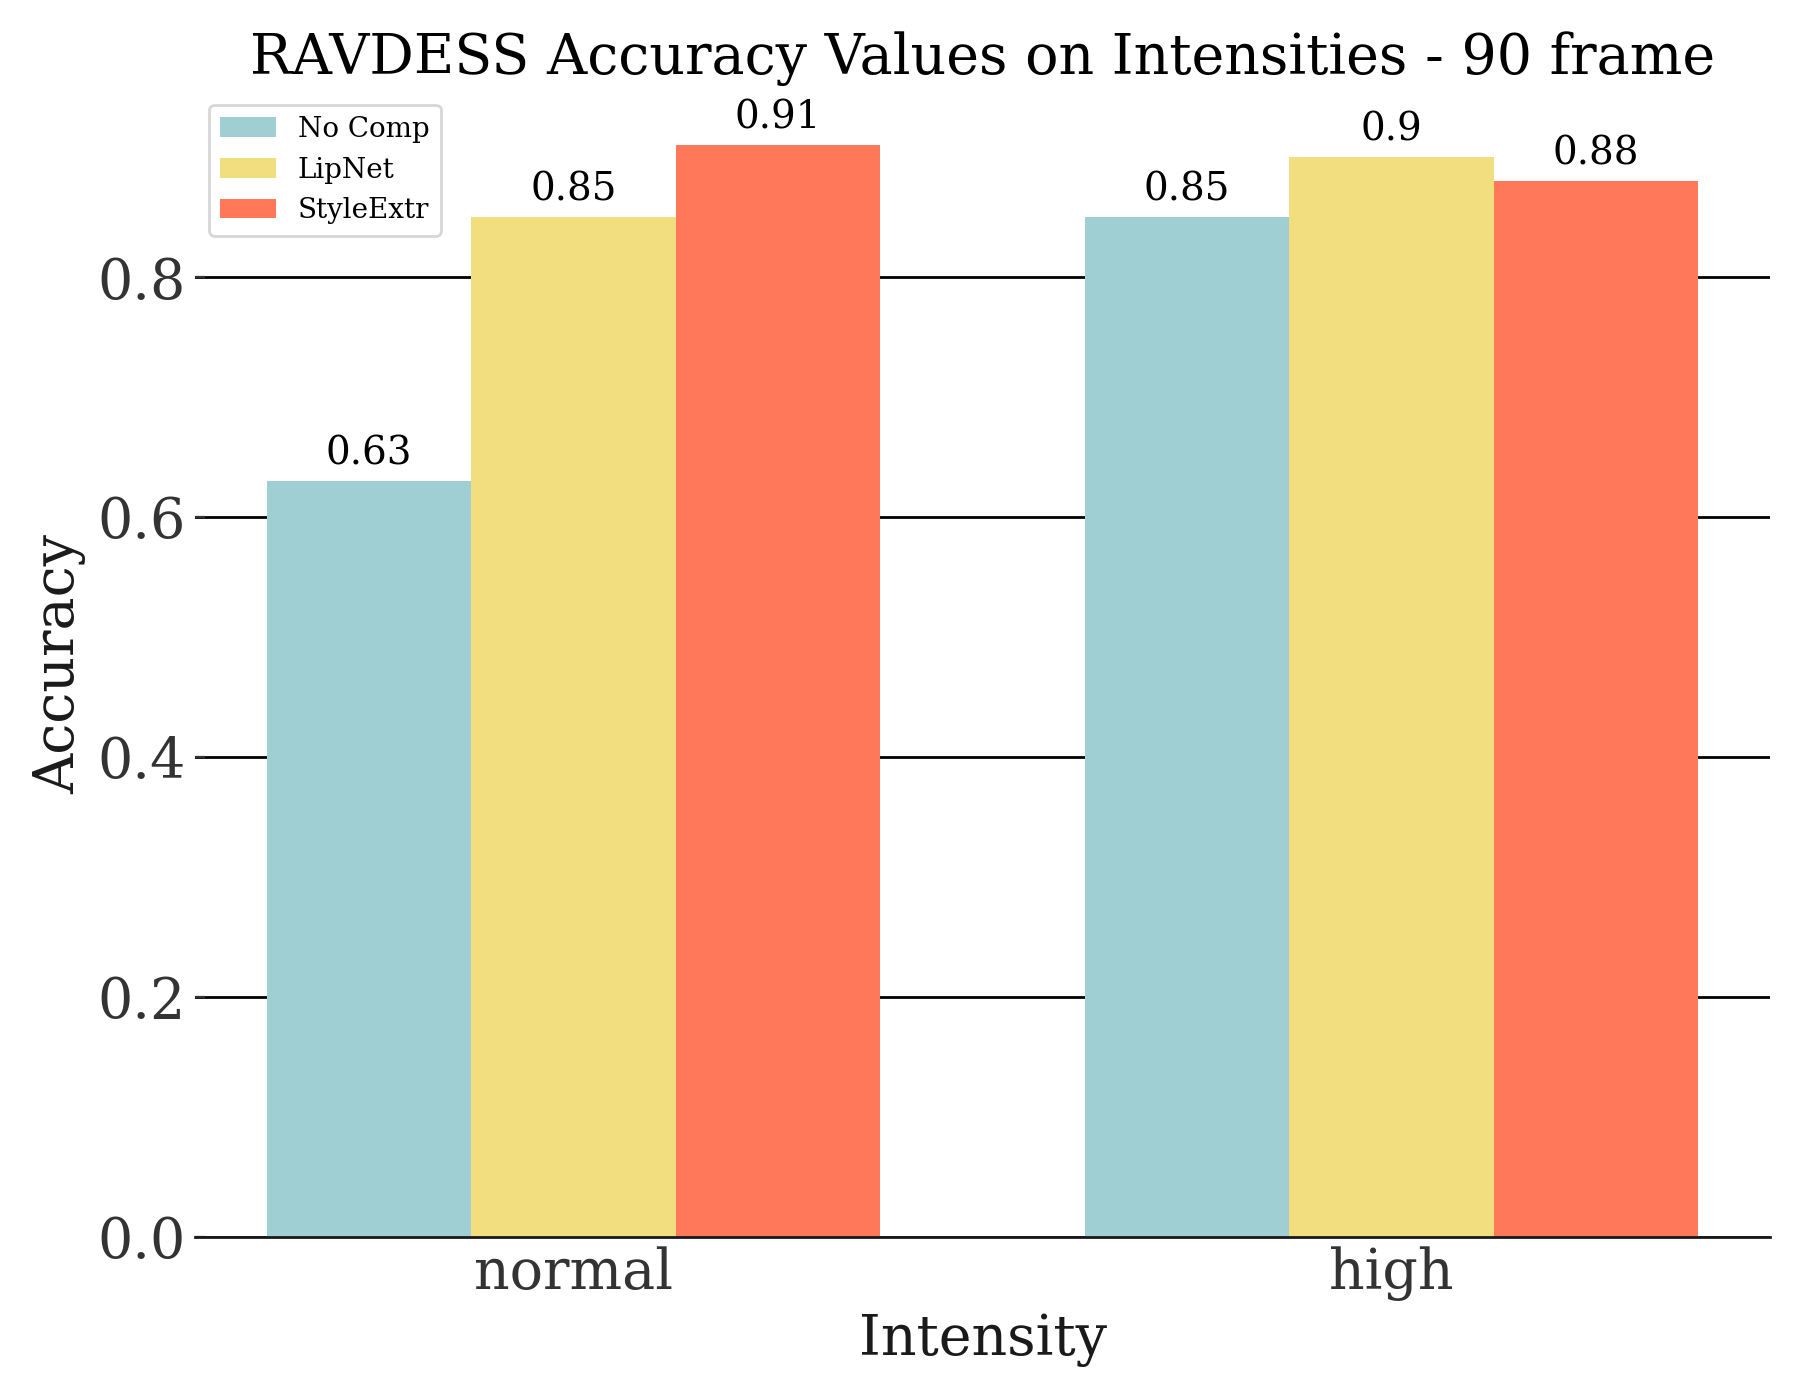
\includegraphics[width=\textwidth]{res/rd-intensities-90.png}
%     \end{subfigure}
%     \caption{Performance of the models based on the intensity value on the RAVDESS validation set. Neutral videos only had a recordings of \texttt{normal} intensity.}
%     \label{fig:rd_intensity}
% \end{figure}


% \FloatBarrier